% !Mode:: "TeX:UTF-8"
%!TEX program  = xelatex
% ============================================================
% 华为杯（中国研究生数学建模竞赛）论文主稿
% 题目：山区洪涝灾害下无人机运输与通信协同优化
% 版式由 gmcmthesis.cls 提供，本文件负责内容组织与门禁标签。
% 编译：XeLaTeX，工作目录为 论文/
% ============================================================
\documentclass[bwprint]{gmcmthesis}

\hypersetup{hidelinks, allcolors=black}

\usepackage{subfig}
\usepackage{siunitx}
\usepackage{multirow}
% 定宽列型：Y 居中、W 左对齐，宽度按文本宽度分数分配，避免越界并保留 tabular 形态
\newcolumntype{Y}[1]{>{\centering\arraybackslash}p{\dimexpr#1\textwidth-2\tabcolsep-\arrayrulewidth\relax}}
\newcolumntype{W}[1]{>{\raggedright\arraybackslash}p{\dimexpr#1\textwidth-2\tabcolsep-\arrayrulewidth\relax}}

% 宽表自适应列类型：C 居中、Z 左对齐，均按剩余宽度自动换行
\newcolumntype{C}{>{\centering\arraybackslash}X}
\newcolumntype{Z}{>{\raggedright\arraybackslash}X}

\setmonofont[Scale=MatchLowercase]{Consolas}

% 附录代码排版：备份模板既有的 Python 代码环境宏，在其设置之后追加一条 lstset，
% 只收紧字号与左右边距以缓解长行折行造成的版面稀疏，配色与结构仍沿用模板定义。
\makeatletter
\let\huaweiPythonBegin\Python
\let\huaweiPythonEnd\endPython
\renewcommand{\Python}[1]{%
  \huaweiPythonBegin{#1}%
  \lstset{basicstyle=\scriptsize\ttfamily,xleftmargin=4pt,xrightmargin=4pt,framesep=2pt}%
}
\renewcommand{\endPython}{\huaweiPythonEnd}
\makeatother


% 图/表全篇连续编号，不随章节重置
\counterwithout{figure}{section}
\counterwithout{table}{section}

% 算法
\usepackage[noend]{algpseudocode}
\usepackage{algorithmicx,algorithm}
\floatname{algorithm}{算法}
\renewcommand{\algorithmicrequire}{\textbf{输入:}}
\renewcommand{\algorithmicensure}{\textbf{输出:}}

% 引用以上标数字角标显示
\makeatletter
\def\@cite#1#2{\textsuperscript{[{#1\if@tempswa , #2\fi}]}}
\makeatother

%===================== 建模论文题目与封面信息 =====================

\title{山区洪涝灾害下无人机运输与通信协同优化}
\baominghao{\hspace{6em} 20260900001}
\schoolname{\hspace{5.8em} 学校名称填写}
\membera{\hspace{6em} 成员A}
\memberb{\hspace{6em} 成员B}
\memberc{\hspace{6em} 成员C}

%=======================================================

\begin{document}
\label{body:start}

\maketitle

\begin{abstract}
\label{abstract:start}
山区洪涝灾害常同时破坏道路、供电与通信设施，使受灾居民点在短时间内失去地面交通联系。本文以广西横州市镇龙乡为背景，围绕临时调度中心 O01 与 15 个服务区、80 个不可拆货箱、三类运输机型共 8 架实体无人机、2 架中继无人机及配套电池与能源组件，建立运输能力、异构调度、通信保障与资源配置四层递进的数学模型，全部参数取自赛题附件。

\textbf{针对问题一}，本文把单点往返能力化为单变量单调方程求根问题，求得\textbf{最大安全载荷}，组批以剩余数量向量为状态做精确动态规划。A 型在 15 个服务区均达额定上限 25.00 kg，B 型除 S008 为 28.63 kg 外均达 30.00 kg，C 型在 5 个服务区受能量约束、最小为 58.43 kg。最少架次方案为 18 架次、能耗 59.261 kWh、累计作业时间 32841.5 s，A 型因容量被 B 型支配而未入选。真实 Pareto 集为 18 与 19 架次，增加 1 个架次仅省 0.098 kWh，故架次数应作为首要目标；全部货箱可投递的临界返航安全余量为 0.3503。

\textbf{针对问题二}，本文建立含载质量、体积、返航余量、机队与电池周转及时限约束的异构多点多架次调度模型，采用分层构造、局部搜索与机型负载再平衡。最优方案含 27 个架次、能耗 86.983 kWh、\textbf{全部任务完成时间 10313.4 s}，首批保障货箱截止时间全部满足。四套权重方案在四项指标上互为非受支配：能耗优先方案比及时性优先方案少耗 8.66 kWh，完成时间多 281.0 s。

\textbf{针对问题三}，本文把架次展开为 5 s 步长轨迹，按附录 3 的地形遮挡、双向链路预算与传播损耗识别链路状态，发现 15 个服务区在投送作业高度上仅 3 个可直连网关，缺口采样点占 39.19\%。以\textbf{贪心集合覆盖}选定 4 个中继悬停位置即可覆盖全部缺口。单架次最大连续服务约 2.2 h，2 架中继无法同时满足首批时限；在 2 至 6 架范围内，首批时限满足与缺口全覆盖无法兼得。

\textbf{针对问题四}，本文以同架次关系图求不可拆分单元并构造\textbf{任务分区}，各任务组独立重跑装箱、合并与调度链路。划分为 2 组需运输无人机 6 架、共享电池 13 组、中继无人机 3 架，缺口仅中继无人机 1 架；划分为 3 组需 9 架与 17 组，缺口增至 5 项，组间工作量不均衡度由 0.053 升至 0.273，故\textbf{2 组分区在资源规模、冗余与均衡三方面均优于 3 组分区}。

综上，本文在能耗、时间与通信约束下给出可复现的协同调度方案，并量化了中继机队规模与分区粒度对资源配置的影响，可为山区洪涝救援的装备编成提供定量依据。

\keywords{无人机应急运输\quad 货箱组批\quad 异构调度\quad 空中中继\quad 通信链路预算\quad 任务分区}\label{abstract:end}

\end{abstract}

\pagestyle{plain}

\maketoc
\clearpage

\section{问题重述}

\subsection{问题背景}
山区洪涝灾害具有突发性强、影响范围分散的特点，连续强降雨可能引发山洪、滑坡与道路塌方，使部分居民点在短时间内失去稳定的地面交通联系。灾后早期，饮用水、应急食品、医疗物资与生活卫生用品需要尽快送达，而传统车辆难以进入地形起伏大、道路受损严重的区域。无人机受地面道路条件影响较小，可作为应急运输的重要补充手段\cite{ref1,ref2}。

2026 年 7 月，受台风带来的持续强降雨影响，广西横州市镇龙乡遭遇严重洪涝灾害，核心受灾区域一度处于交通中断、通信不畅状态，全乡约 8000 人受困\cite{ref2}。救援期间，食品、饮用水与药品依靠徒步或空中投送进入受灾区域，大型无人机承担电力抢修材料运输，临时通信设备与应急供电设备用于逐步恢复灾区联络。这一场景表明，应急物资运输与通信保障往往需要在道路受阻、能源受限与信息不完整的条件下协同组织。

完成物资投送不仅取决于无人机能否飞抵目标区域，还受载荷、水平飞行距离、爬升与下降高度、沿线地形净空、能源储备、任务时限与设备周转等因素影响。运输无人机在爬升、巡航、下降及物资交接的全过程中需要持续保持指挥、遥测与交接确认链路。当固定通信设施受损，或山体遮挡导致地面网关无法覆盖完整任务区间时，还需要空中中继无人机在适当的位置和时段提供临时通信保障\cite{ref8}。因此，山区洪涝灾害下的物资投送同时涉及运输组织与通信保障，并需要同步考虑设备资源的协调使用。

本文以镇龙乡及周边山区为标准测试场景。附件提供 1 个临时调度中心 O01、15 个服务区与 80 个不可拆货箱，设置三种运输无人机机型，共配置 8 架实体运输无人机，并给出配套共享电池组、30 米数字高程模型数据、中继无人机、可更换能源组件及无线链路参数。空间坐标与公开地理数据用于描述测试场景，需求、时限、装备与资源参数一律以附件给定值为准。

\subsection{问题提出}
题面围绕运输任务如何组织、通信保障如何匹配以及有限资源如何合理调配，提出四个递进的问题。

问题一在不考虑实体无人机与共享电池调度的前提下，研究单服务区由调度中心 O01 直飞某一服务区再原路返回的运输能力与货箱组批。要求计算三种机型在 15 个服务区的最大安全载荷；在货箱不可拆、每箱只安排一次、不跨服务区组批且满足载质量、装载体积与返航安全能量余量的条件下确定组批方案；以往返架次数、总运输能耗与累计作业时间为指标优化并说明权衡关系；讨论返航安全余量变化对最大安全载荷与组批结果的影响。

问题二在不考虑通信保障的前提下，研究异构运输无人机的多点多架次调度。每个架次可访问一个或多个服务区并在完成交付后返回 O01。要求在满足货箱不可拆、载质量与装载体积、返航安全余量、无人机与共享电池数量、充电周转及物资时限等约束下，联合确定货箱组批、服务区访问顺序、运输机型、具体执行无人机、共享电池及各架次开始时刻，并综合考虑配送及时性、全部任务完成时间、运输能耗与架次数进行优化。

问题三在考虑通信保障的前提下，研究运输无人机与中继无人机的联合调度。运输无人机在爬升、巡航、下降及物资投送阶段均应保持连续通信；与固定网关直连不可用时，可由空中中继无人机提供通信保障。要求在满足货箱时限、载荷与能量、连续通信及资源可用性等约束下，联合确定货箱组批与访问顺序、运输无人机及共享电池安排、各架次开始时刻，以及中继无人机的悬停位置、飞行海拔、服务时段与能源组件分配。

问题四研究救援任务分区与资源配置。以问题三得到的联合调度方案为基础，分别将 15 个服务区划分为 2 个和 3 个任务组，每个服务区必须且只能属于一个任务组，每个任务组至少包含一个服务区；分区过程保持问题三已确定的货箱组批、服务区访问顺序、运输与中继任务安排及通信保障关系不变，若同一运输架次同时涉及多个服务区则这些服务区应划入同一任务组。要求分别给出两种分区的任务分区与资源配置方案，并从资源配置规模、资源冗余、组间工作量均衡以及与现有库存之间的资源缺口等方面进行比较，对超出库存的方案给出缺口及其原因。

\subsection{问题分析}
四个问题构成由单点能力到全局协同、再到资源编成的递进链条，其耦合关系与数据继承关系如图~\ref{fig:analysis} 所示。

\begin{figure}[htbp]
\centering
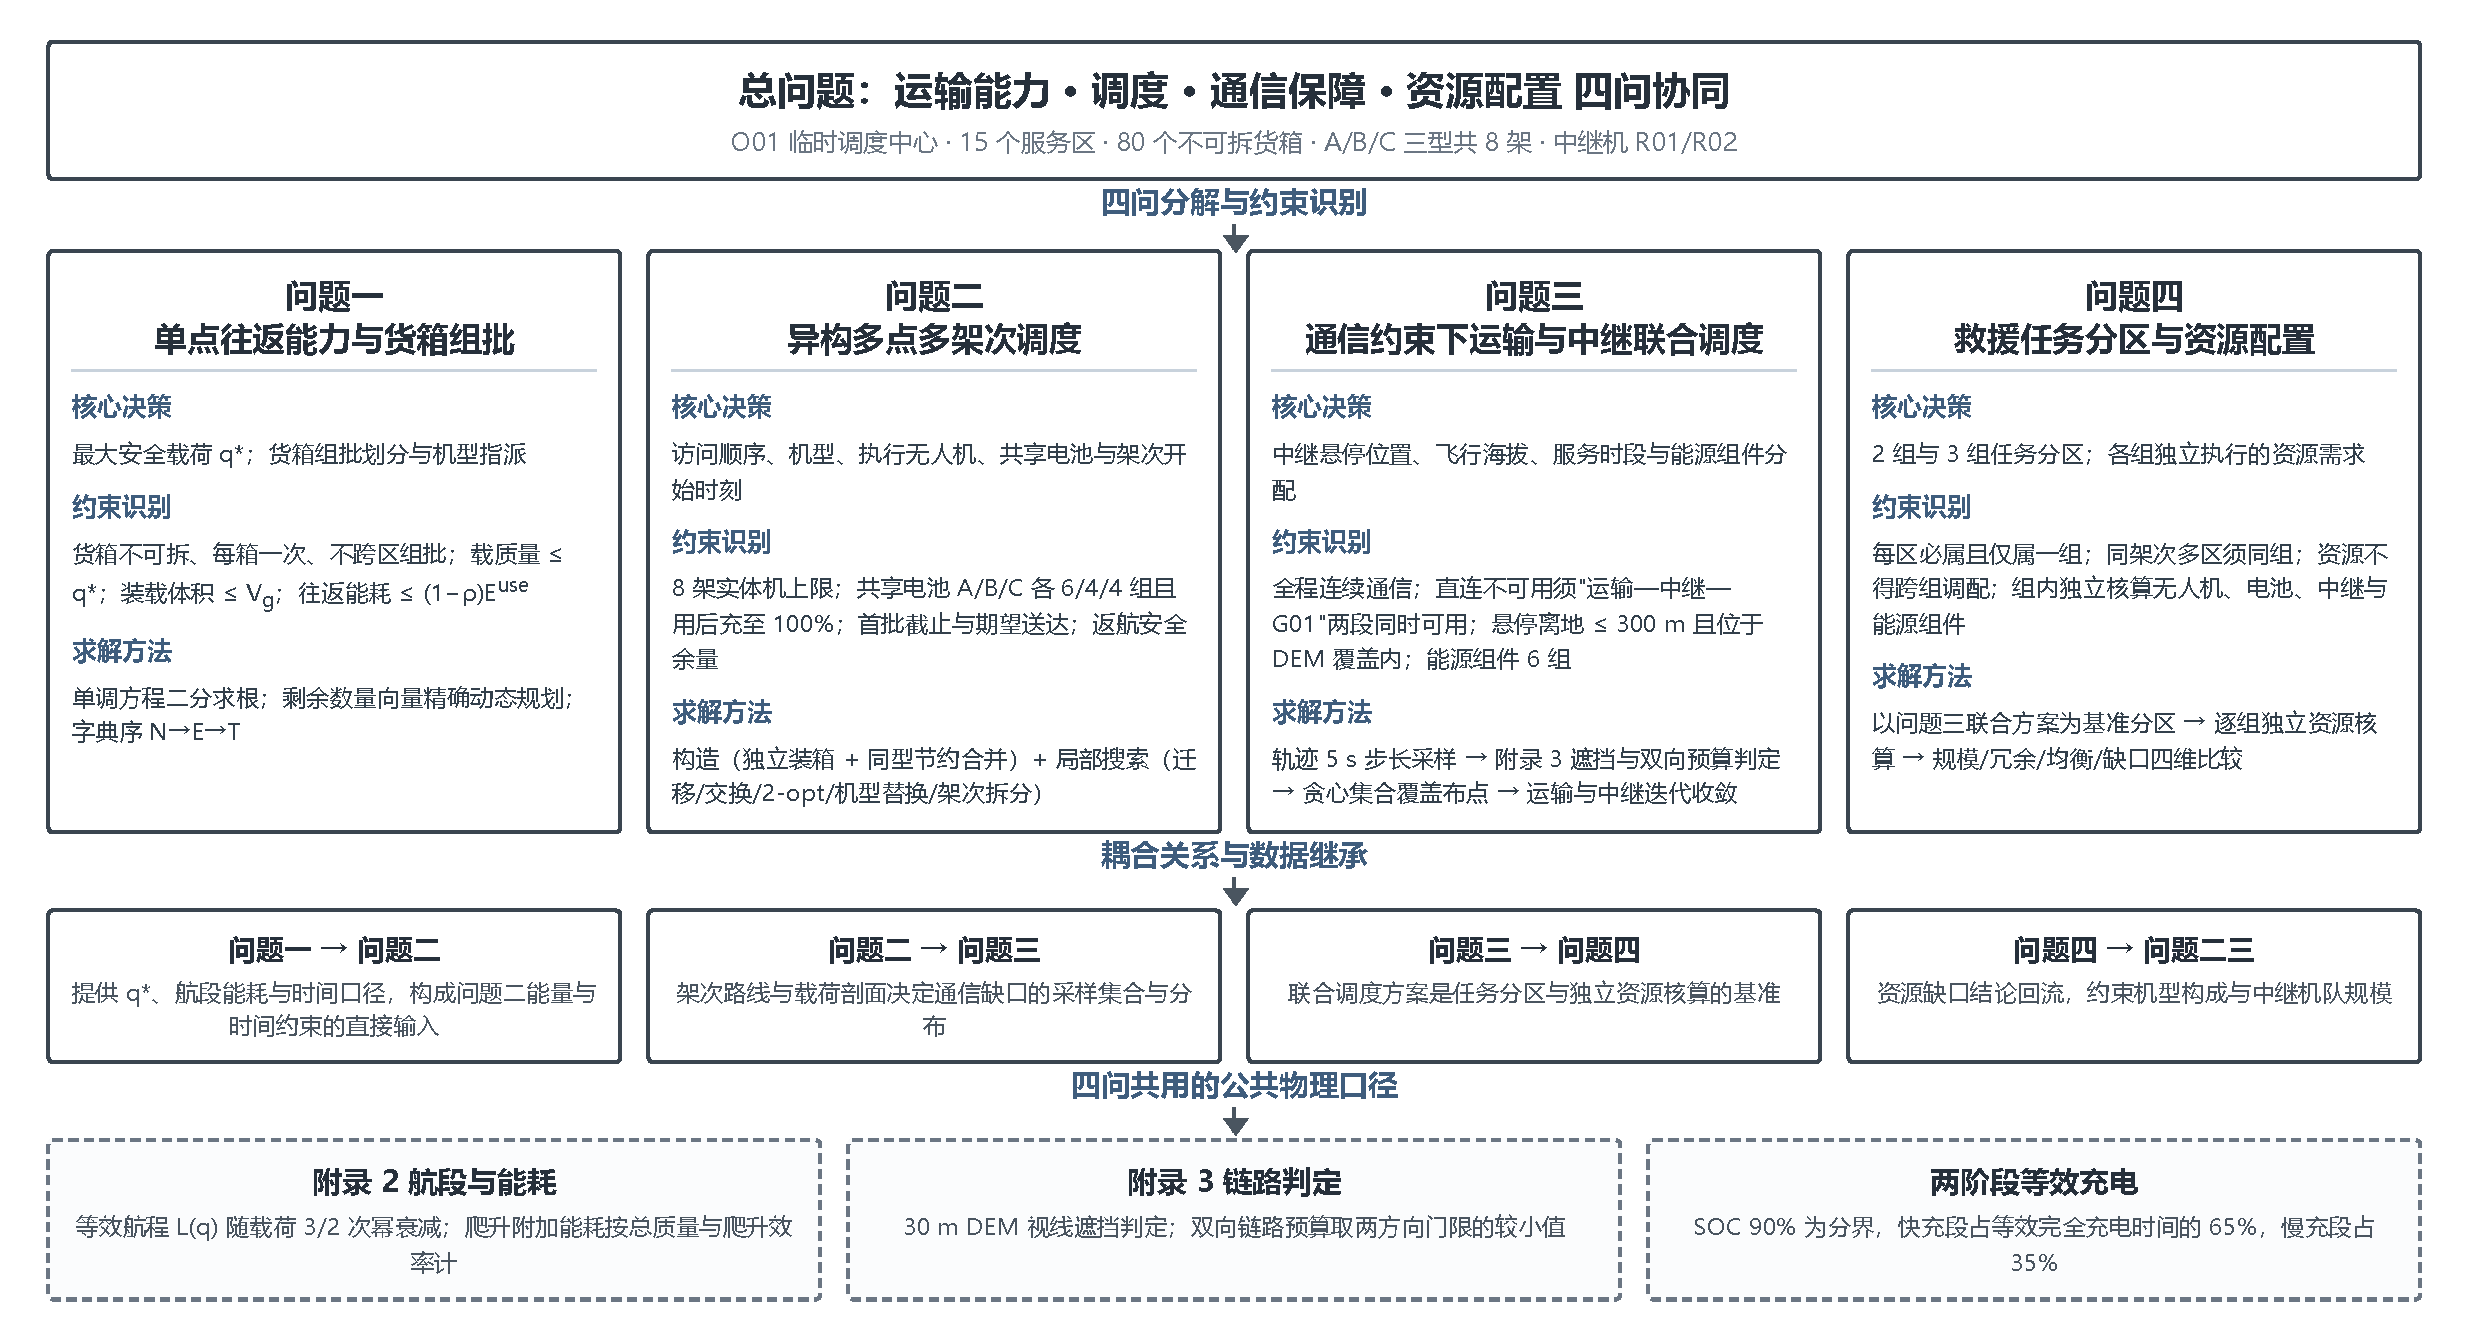
\includegraphics[width=\textwidth]{../手绘图/问题分析流程图.pdf}
\caption{四问的问题分解、约束识别与耦合继承关系}
\label{fig:analysis}
\end{figure}

四问共用同一套物理口径：航段水平距离按两节点球面大圆距离计算，计划巡航海拔取航段沿途 30 米 DEM 像元最高地面高程以上 50 米，航段能耗分解为水平巡航能耗与爬升附加能耗；链路状态按 30 米 DEM 视线遮挡、双向链路预算取两方向最大允许传播损耗的较小值，再与含遮挡附加损耗的总传播损耗比较；两类能源资源统一采用以荷电状态 90\% 为分界的两阶段等效充电模型。这套口径贯穿全部四问，保证对象编号、单位与计算口径一致。

问题一给出最大安全载荷、航段能耗与航段时间，构成问题二能量约束与时间约束的直接输入。问题二的架次路线与载荷剖面决定通信缺口的采样集合与分布，是问题三链路状态判断的输入。问题三的联合调度方案是问题四任务分区与独立资源核算的基准。问题四得到的资源缺口结论回流至问题二与问题三，约束机型构成与中继机队规模的配置方向。整体技术路线如图~\ref{fig:roadmap} 所示。

\begin{figure}[htbp]
\centering

\includegraphics[width=\textwidth]{../手绘图/技术路线图.pdf}
\caption{全文技术路线与结论回流关系}
\label{fig:roadmap}
\end{figure}

数据方面，节点坐标与地面海拔取自调度中心与服务区附件，经与 30 米 DEM 采样值逐点比较，最大绝对偏差 16.2 m、平均绝对偏差 3.9 m，量级与栅格分辨率及点位代表性相符。按题面口径，节点地面海拔以附件给定值为准，DEM 仅承担地形净空、巡航海拔与视线遮挡识别。服务区距调度中心水平距离介于 2.82 km 与 8.11 km 之间，海拔介于 127.7 m 与 444.5 m 之间，DEM 高程介于 41.7 m 与 1132.9 m 之间，地形起伏剧烈。图~\ref{fig:dem} 给出 30 米 DEM 高程场与 16 个调度节点的空间关系。

\begin{figure}[htbp]
\centering
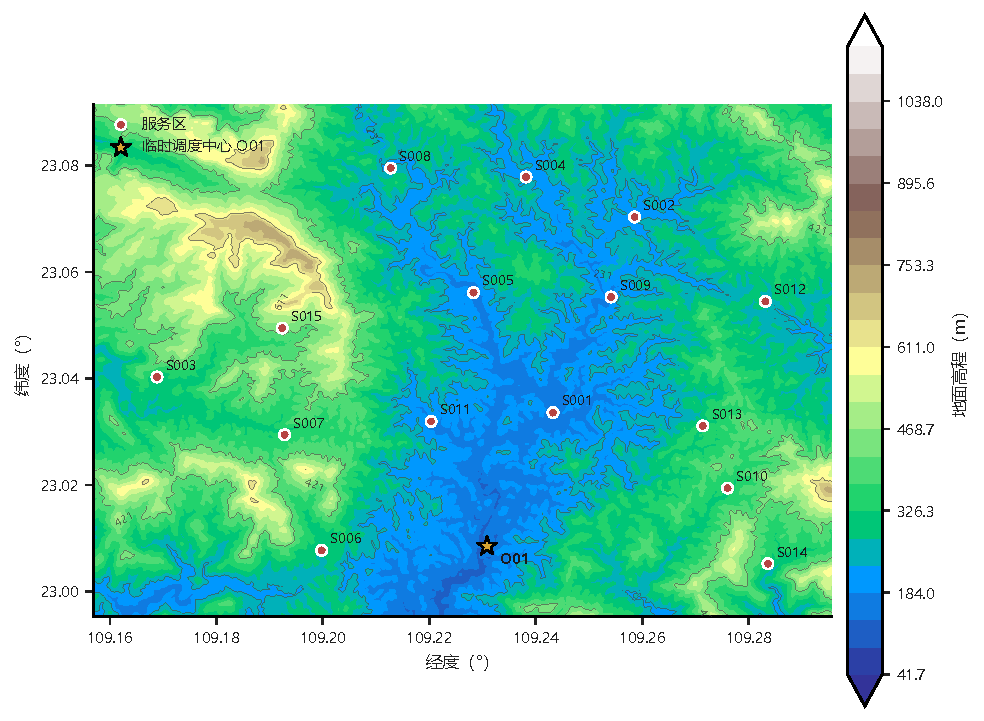
\includegraphics[width=0.86\textwidth]{../数据预处理/figures/fig_eda_dem_nodes.pdf}
\caption{30 米 DEM 地面高程场与 16 个调度节点的空间关系}
\label{fig:dem}
\end{figure}

图中可见调度中心 O01 位于中部偏南的低海拔河谷，服务区 S003、S007、S015 分布在西部与北部的高海拔山区，S014、S010 位于东南部。高程跨度接近 1100 m 意味着航段爬升高度与视线遮挡都会对运输能耗和通信可用性产生实质影响，这也解释了后文为何必须显式建模爬升附加能耗与地形遮挡。

80 个货箱总质量 758.0 kg、总体积 2.042 m$^3$，单箱质量介于 3 kg 与 14 kg 之间，单箱体积介于 0.012 m$^3$ 与 0.035 m$^3$ 之间，其中首批保障货箱 25 箱。需求在服务区之间高度不均衡，图~\ref{fig:demand} 给出服务区需求总质量、保障人口与空间距离的关系。

\begin{figure}[htbp]
\centering
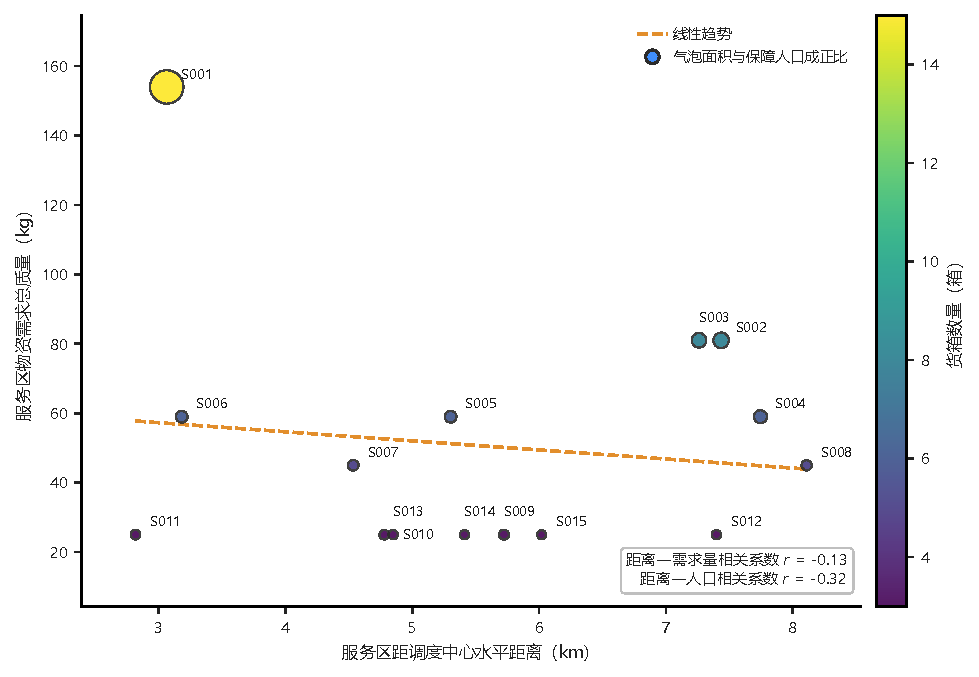
\includegraphics[width=0.86\textwidth]{../数据预处理/figures/fig_eda_demand_structure.pdf}
\caption{服务区需求规模、保障人口与空间距离的关系}
\label{fig:demand}
\end{figure}

S001 单个服务区需求 155 kg，占全部需求的 20.4\%，保障人口 2100 人；而 S015 仅 15 kg、保障人口 3 人。需求总质量与空间距离的相关系数为 $-0.13$，与保障人口的相关系数为 $-0.32$，说明需求规模并非由距离决定，组批方案必须按服务区差异化配置而不能套用统一架次模板。这一结论直接决定了问题一中组批模型必须以服务区为单位独立求解。

\section{模型假设与符号说明}

\subsection{模型假设}
结合题面口径、附件数据特征与建模需要，本文采用以下假设。

\begin{enumerate}
\item 同一服务区内、同一物资类型、同一首批保障属性的货箱在质量与体积上完全同质，可视为同类物品。该假设由数据预处理阶段逐项核对，同类货箱的质量与体积在各服务区之间保持一致。
\item 运输架次采用两节点水平直线航段，计划巡航海拔取该航段沿途 30 米 DEM 像元最高地面高程以上 50 m；调度中心作业高度取其地面海拔，服务区作业高度取其地面海拔以上 30 m，连续访问多个服务区时每次投送后均从 30 m 作业高度重新爬升。
\item 航段能耗分解为水平巡航能耗与爬升附加能耗，下降阶段不单独计算附加能耗，与题面给定下降能耗效率为零一致。
\item 机型携带载荷 $q$ 时的等效航程按题面给定的 $3/2$ 次幂关系衰减，水平巡航单位距离能耗按单组电池可用能量除以等效航程折算。
\item 架次作业时间由工位固定准备时间、逐箱装载时间、各航段飞行时间与接收点交接时间构成，交接时间随投送箱数线性增加。
\item 共享电池与中继能源组件均按独立资源记录荷电状态，同一机型共享电池可在该机型不同实体无人机之间调度，不同机型之间不混用；资源用后须充至 100\% 才能再次投入任务，充电时间按以荷电状态 90\% 为分界的两阶段等效模型折算。
\item 通信链路按双向判断，链路门限取两个通信方向最大允许传播损耗中的较小值；地形遮挡按 30 米 DEM 判断视线连线是否被沿途地形阻断，遮挡成立时计入固定附加损耗。
\item 每架运输无人机在任一时刻只能由固定网关或一架中继无人机提供通信保障，不允许中继无人机之间多跳转发。
\item 中继无人机悬停位置位于所给 DEM 覆盖范围内，悬停离地高度不超过附件规定上限；中继往返悬停位置的地形净空按与运输航段相同的规则确定。
\item 问题四中各任务组仅承担本组服务区对应的运输与通信保障任务，任务执行期间各类资源不得跨组调配；分区后各组按同一套装箱、合并与调度规则独立重新组批。
\end{enumerate}

\subsection{符号说明}
本文全部符号在四问之间保持统一。符号表中只列出贯穿全文的主符号，各问特有的中间量在对应章节就地定义。

\renewcommand\arraystretch{1.2}
\newcolumntype{P}[1]{>{\centering\arraybackslash}p{#1}}
\renewcommand\arraystretch{1.2}
\newcolumntype{P}[1]{>{\centering\arraybackslash}p{#1}}
% 符号内容超过一页，按模板说明改用 longtable：自动跨页并重复表头，
% 进入前保存 table 计数、结束后恢复，使符号表不占用正式结果表编号。
\newcounter{huaweisymbolsavetable}
\setcounter{huaweisymbolsavetable}{\value{table}}
\begin{longtable}{|P{1.6cm}|>{\raggedright\arraybackslash}p{\dimexpr0.9\textwidth-1.6cm-4\tabcolsep-3\arrayrulewidth\relax}|}
  \hline
  符号    &   \quad 意义 \\
  \hline
  \endfirsthead
  \hline
  符号    &   \quad 意义（续） \\
  \hline
  \endhead
  $g$  &  运输机型编号，$g\in\{A,B,C\}$    \\
  \hline
  $i,j$  &  任务节点编号，$O01$ 为临时调度中心，$S001\sim S015$ 为服务区    \\
  \hline
  $q$  &  架次或航段的有效载荷，单位 kg    \\
  \hline
  $Q_g$  &  机型 $g$ 的最大载货质量，单位 kg    \\
  \hline
  $V_g$  &  机型 $g$ 的可用装载体积，单位 m$^3$    \\
  \hline
  $L_g(q)$  &  机型 $g$ 携带载荷 $q$ 时的等效航程，单位 m    \\
  \hline
  $L_g^{0},L_g^{F}$  &  机型 $g$ 的空载与满载标准航程，单位 m    \\
  \hline
  $E_g^{use}$  &  机型 $g$ 单组电池的可用能量，单位 kWh    \\
  \hline
  $\rho_g$  &  机型 $g$ 的返航安全余量比例    \\
  \hline
  $d_{ij}$  &  节点 $i$ 到节点 $j$ 的水平巡航距离，单位 m    \\
  \hline
  $h_{ij}^{+},h_{ij}^{-}$  &  航段的爬升高度与下降高度，单位 m    \\
  \hline
  $v_g^{\uparrow},v_g^{c},v_g^{\downarrow}$  &  机型 $g$ 的爬升、巡航与下降速度，单位 m/s    \\
  \hline
  $\eta_g^{\uparrow}$  &  机型 $g$ 的爬升能耗效率    \\
  \hline
  $m_g$  &  机型 $g$ 的含电池空载总质量，单位 kg    \\
  \hline
  $E_{ij}^{g}(q)$  &  机型 $g$ 在航段 $i\to j$ 上携带载荷 $q$ 的能耗，单位 kWh    \\
  \hline
  $q^{*}_{g,i}$  &  机型 $g$ 在服务区 $i$ 的最大安全载荷，单位 kg    \\
  \hline
  $N,E,T$  &  往返架次数、总运输能耗与累计作业时间，单位分别为架次、kWh、s    \\
  \hline
  $p$  &  运输架次编号    \\
  \hline
  $K_g$  &  机型 $g$ 配置的实体无人机架数    \\
  \hline
  $B_g$  &  机型 $g$ 的共享电池组数量    \\
  \hline
  $s$  &  电池或能源组件任务结束时的荷电状态    \\
  \hline
  $T^{full}$  &  相应能源资源的等效完全充电时间，单位 s    \\
  \hline
  $t^{chg}(s)$  &  由荷电状态 $s$ 充至 100\% 所需时间，单位 s    \\
  \hline
  $f$  &  载波频率，单位 MHz    \\
  \hline
  $D_{ij}(t)$  &  时刻 $t$ 两个通信端点之间的三维直线距离，单位 km    \\
  \hline
  $b_{ij}(t)$  &  地形遮挡变量，取 1 表示存在遮挡    \\
  \hline
  $L^{obs}$  &  地形遮挡附加损耗，单位 dB    \\
  \hline
  $L^{\max}_{a\leftrightarrow b}$  &  端点 $a$ 与 $b$ 之间的双向链路门限，单位 dB    \\
  \hline
  $A_{ij}(t)$  &  链路可用性变量，取 1 表示链路可用    \\
  \hline
  $\mathcal{G}_k$  &  第 $k$ 个任务组的服务区集合    \\
  \hline
\end{longtable}
\setcounter{table}{\value{huaweisymbolsavetable}}


\section{问题一模型建立与求解}

\subsection{问题分析与模型建立}
本问的决策对象是单服务区直接往返架次。由于每个架次只服务一个服务区且去程载货、回程空载，问题可分解为两个层次：先确定给定机型在给定服务区的载荷上界，再在该上界下把货箱划分为若干架次并优化指标。图~\ref{fig:q1flow} 给出求解流程。

\begin{figure}[htbp]
\centering

\includegraphics[width=\textwidth]{../手绘图/组批求解流程图.pdf}
\caption{问题一的单点往返能力求解与组批精确动态规划流程}
\label{fig:q1flow}
\end{figure}

\subsubsection{航段几何与能耗口径}
节点 $i$ 的作业高度 $a_i$ 按题面口径确定，调度中心取地面海拔，服务区取地面海拔以上 30 m。航段 $i\to j$ 的水平距离按球面大圆距离计算，计划巡航海拔取该航段沿途 DEM 像元最高地面高程以上 50 m，记为 $H_{ij}$，则爬升高度与下降高度分别为
\begin{equation}
h_{ij}^{+}=\max\left(H_{ij}-a_i,\,0\right),\qquad
h_{ij}^{-}=\max\left(H_{ij}-a_j,\,0\right).
\end{equation}

航段飞行时间由爬升、巡航与下降三段构成，
\begin{equation}
t_{ij}^{g}=\frac{h_{ij}^{+}}{v_g^{\uparrow}}+\frac{d_{ij}}{v_g^{c}}+\frac{h_{ij}^{-}}{v_g^{\downarrow}}.
\label{eq:segtime}
\end{equation}

等效航程按题面给定关系随载荷衰减，
\begin{equation}
L_g(q)=L_g^{0}-\left(L_g^{0}-L_g^{F}\right)\left(\frac{q}{Q_g}\right)^{3/2},\qquad 0\le q\le Q_g .
\label{eq:range}
\end{equation}
该式的含义是载荷越重，单组电池能够水平飞行的距离越短，且衰减速度快于线性，因此大载荷航段对能量预算的挤占比按质量比例估算更为严重。

航段能耗按水平巡航能耗与爬升附加能耗之和计算，
\begin{equation}
E_{ij}^{g}(q)=\underbrace{E_g^{use}\cdot\frac{d_{ij}}{L_g(q)}}_{\text{水平巡航}}
+\underbrace{\frac{\left(m_g+q\right)\rho_{e}\,h_{ij}^{+}}{3.6\times10^{6}\,\eta_g^{\uparrow}}}_{\text{爬升附加}},
\label{eq:segenergy}
\end{equation}
其中 $\rho_e$ 为重力加速度取值 9.8 m/s$^2$，分母中的换算因子把焦耳折算为千瓦时。水平巡航项把单组电池全部可用能量按等效航程摊到本航段实际距离上，爬升附加项把总质量抬升 $h_{ij}^{+}$ 所需的势能除以爬升效率。下降阶段不单独计附加能耗，与题面给定的下降能耗效率为零一致。

\subsubsection{最大安全载荷}
单点往返的去程载货、回程空载，故架次总能耗为
\begin{equation}
E_{i}^{rt}(q)=E_{O01,i}^{g}(q)+E_{i,O01}^{g}(0).
\label{eq:rtenergy}
\end{equation}
返航安全余量约束要求架次总能耗不超过单组电池可用能量的 $1-\rho_g$ 倍，
\begin{equation}
E_{i}^{rt}(q)\le\left(1-\rho_g\right)E_g^{use}.
\label{eq:reserve}
\end{equation}
由式~\eqref{eq:range} 知 $L_g(q)$ 关于 $q$ 单调递减，故式~\eqref{eq:segenergy} 的水平巡航项关于 $q$ 单调递增；爬升附加项含因子 $m_g+q$，同样关于 $q$ 单调递增。两项之和使 $E_{i}^{rt}(q)$ 在 $[0,Q_g]$ 上严格单调递增，于是式~\eqref{eq:reserve} 的可行载荷构成一个下闭区间，最大安全载荷
\begin{equation}
q^{*}_{g,i}=\max\left\{q\in[0,Q_g]\;\middle|\;E_{i}^{rt}(q)\le\left(1-\rho_g\right)E_g^{use}\right\}
\label{eq:qstar}
\end{equation}
可由二分法唯一确定。这一单调性是本问能够用简单求根替代一般非线性规划的关键，也是后文把载荷上界直接当作组批容量约束的依据。

\subsubsection{货箱组批的精确动态规划}
在 $q^{*}_{g,i}$ 确定后，组批问题为带容量与能量约束的装箱问题。由于货箱不可拆、每箱只安排一次且不跨服务区组批，各服务区之间相互独立，可逐区求解。

同一服务区内、同一物资类型、同一首批保障属性的货箱在质量与体积上完全同质，因此可以按类别归并。设服务区 $i$ 的货箱归并为 $K_i$ 个类别，第 $k$ 类含 $c_k$ 件、单件质量 $m_k$、单件体积 $u_k$。以各类物品的剩余数量向量 $\mathbf{r}=(r_1,\dots,r_{K_i})$ 为状态，状态空间规模为 $\prod_k(c_k+1)$。动作是一次架次，由机型 $g$ 与各类物品取用数量向量 $\mathbf{x}$ 刻画，须满足
\begin{equation}
\sum_{k} x_k m_k\le q^{*}_{g,i},\qquad \sum_{k} x_k u_k\le V_g,\qquad \mathbf{0}\ne\mathbf{x}\le\mathbf{r}.
\label{eq:batchcons}
\end{equation}
状态转移为 $\mathbf{r}\to\mathbf{r}-\mathbf{x}$，转移代价为架次能耗 $E_{i}^{rt}\!\left(\sum_k x_k m_k\right)$ 与架次作业时间 $\tau_g(n)$，其中
\begin{equation}
\tau_g(n)=\tau_g^{prep}+n\,\tau_g^{load}+t_{O01,i}^{g}+t_{i,O01}^{g}+\tau_g^{h0}+n\,\tau_g^{h1},
\label{eq:sortietime}
\end{equation}
式中 $n=\sum_k x_k$ 为该架次投送箱数，前两项为工位准备与逐箱装载，中间两项为往返飞行，末两项为接收点基础交接与逐箱增加交接。

以最低位未覆盖物品为规范元，可避免同一划分被重复枚举。设 $\ell(\mathbf{r})$ 为 $\mathbf{r}$ 中序号最小的非零分量，只考虑取用该分量的架次模式，则递推为
\begin{equation}
F(\mathbf{r})=\min_{\mathbf{x}:\,\ell(\mathbf{r})\in\mathrm{supp}(\mathbf{x})}\Big\{\,\mathbf{cost}(\mathbf{x})+F(\mathbf{r}-\mathbf{x})\Big\},
\label{eq:dp}
\end{equation}
边界条件为 $F(\mathbf{0})=\mathbf{0}$。由于状态空间覆盖全部可达剩余数量向量且每个划分恰好被枚举一次，式~\eqref{eq:dp} 给出的是精确最优解而非启发式近似。

\subsubsection{三指标与字典序目标}
本问的三个指标为往返架次数、总运输能耗与累计作业时间，分别记为
\begin{equation}
N=\sum_{p}\mathbf{1},\qquad E=\sum_{p}E_{i(p)}^{rt}\!\left(q_p\right),\qquad T=\sum_{p}\tau_{g(p)}\!\left(n_p\right).
\label{eq:threeobj}
\end{equation}
三个指标量纲不同且未必同向，本文以字典序目标求解：分别按 $N\to E\to T$、$E\to N\to T$ 与 $T\to N\to E$ 三种优先序求最优，再在恰好使用 $N$ 个架次的约束下逐层求最小能耗，得到完整的 $(N,E,T)$ 前沿，并按支配关系提取真实 Pareto 集。采用字典序而非加权和的原因在于三个指标的量纲与数量级差异较大，权重选择会直接影响结论，而字典序解的语义明确、便于比较。

\subsubsection{返航安全余量灵敏度与临界值}
返航安全余量 $\rho$ 同时影响载荷上界与组批结果，本文在 $0.10$ 至 $0.40$ 范围内以 $0.01$ 为步长扫描。由于 $\rho$ 增大使式~\eqref{eq:reserve} 的右端下降，$q^{*}_{g,i}$ 随 $\rho$ 单调不增。当某一服务区的最重货箱质量超过该区全部机型的 $q^{*}$ 时，该区货箱不可投递，模型整体不可行。本文据此对可行性作二分，求出全部货箱可投递的临界返航安全余量 $\rho_c$。

\subsection{求解结果与分析}
按式~\eqref{eq:qstar} 对 3 机型与 15 服务区共 45 个组合二分求根。关键结果为：A 型在全部 15 个服务区均达到额定上限 25.00 kg，B 型除 S008 为 28.63 kg 外均达 30.00 kg，C 型在 S002、S003、S004、S008、S012 五个服务区受能量约束，最小为 S008 的 58.43 kg。完整结果见附录表~\ref{tab:appq1}。



附录表中占比为满载往返能耗与返航能量上限之比，取值大于 1 表示载荷受能量约束。A 型在 15 个服务区的占比最大值为 0.944，B 型仅 S008 一处为 1.031，C 型在 S002、S003、S004、S008、S012 五处超过 1，最大值 1.261 出现在 S008。可见 A 型与 B 型的瓶颈是额定载质量与装载体积而非电池能量，C 型才是唯一在部分服务区受能量约束的机型。

图~\ref{fig:q1payload} 给出三种机型的最大安全载荷随返航安全余量的响应。

\begin{figure}[htbp]
\centering
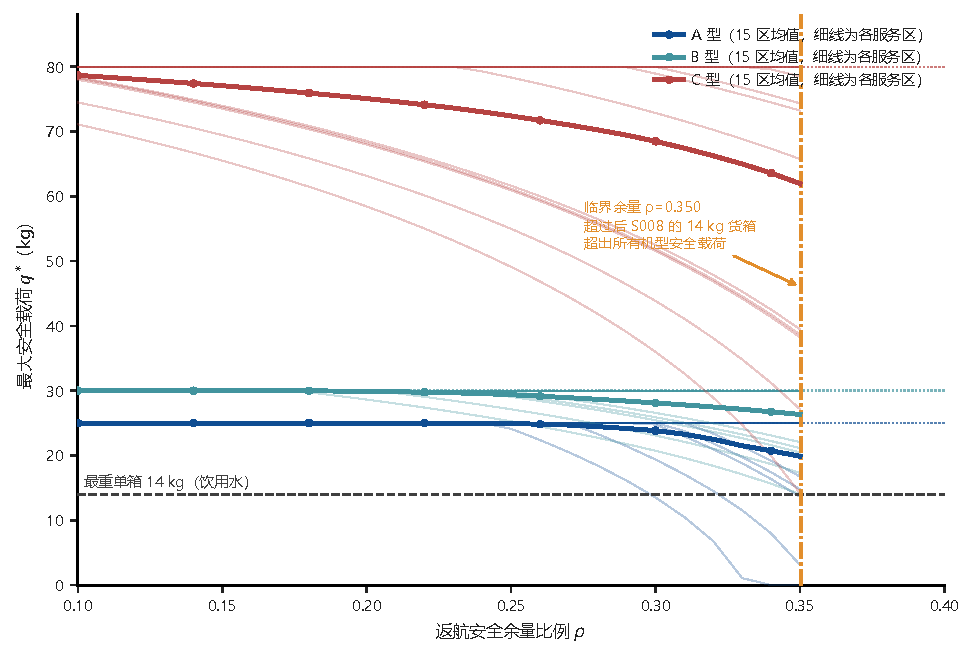
\includegraphics[width=0.88\textwidth]{../Q1/figures/fig_q1_payload_rho.pdf}
\caption{三种机型最大安全载荷随返航安全余量的响应}
\label{fig:q1payload}
\end{figure}

图中粗线为 15 个服务区的均值，细线为各服务区取值，水平虚线为各机型额定载货质量，黑色虚线为最重单箱 14 kg。A 型在 $\rho\le0.24$ 内保持 25.00 kg 不变，B 型在 $\rho\le0.17$ 内保持 30.00 kg 不变，二者在低余量区间完全不受能量约束；C 型均值由 $\rho=0.10$ 时的 78.68 kg 单调降至 $\rho=0.35$ 时的 61.98 kg，衰减幅度 21.3\%。橙色点划线标出临界返航安全余量 $\rho_c=0.3503$，超过该值后 S008 的 14 kg 饮用水货箱超出全部机型的最大安全载荷，该区物资不可投递。

按式~\eqref{eq:dp} 逐区求解组批，字典序 $N\to E\to T$ 的最优方案为 18 个往返架次、总运输能耗 59.261 kWh、累计作业时间 32841.5 s，机型构成为 C 型 12 架次与 B 型 6 架次，A 型未进入最优方案。图~\ref{fig:q1batching} 给出各服务区的架次构成与分区能耗。

\begin{figure}[htbp]
\centering
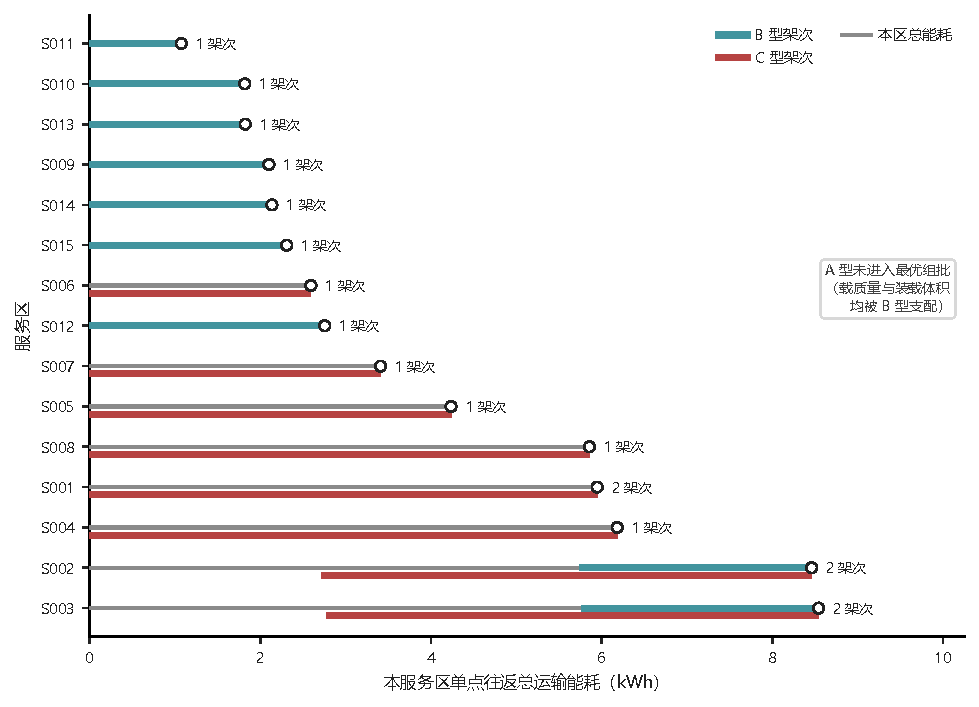
\includegraphics[width=0.88\textwidth]{../Q1/figures/fig_q1_batching.pdf}
\caption{各服务区组批方案的机型构成、分区能耗与架次数}
\label{fig:q1batching}
\end{figure}

图中灰色基线为本区单点往返总能耗，彩色线段按机型分层给出各机型的能耗贡献，端点圆点为架次终止位置。S001、S002、S003 各需 2 个架次，其余 12 个服务区各需 1 个架次。分区能耗最高为 S003 的 8.543 kWh，最低为 S011 的 1.076 kWh，相差 7.9 倍。A 型未被选中，原因是 B 型在载质量 30 kg 与装载体积 0.073 m$^3$ 两个维度上均严格优于 A 型的 25 kg 与 0.06 m$^3$，而单点往返条件下两者的作业时间与能耗差异不足以抵消容量劣势。

三套字典序目标的结果对比如表~\ref{tab:q1lex} 所示。

\begin{table}[htbp]
\centering
\caption{三套字典序目标的求解结果对比}
\label{tab:q1lex}
\renewcommand\arraystretch{1.15}
\begin{tabular}{|c|c|c|c|}
  \hline
  字典序目标 & 往返架次数/架次 & 总运输能耗/kWh & 累计作业时间/s \\
  \hline
  $N\to E\to T$ & 18 & 59.261 & 32841.5 \\
  \hline
  $E\to N\to T$ & 19 & 59.163 & 34509.5 \\
  \hline
  $T\to N\to E$ & 18 & 59.261 & 32841.5 \\
  \hline
\end{tabular}
\end{table}

图~\ref{fig:q1tradeoff} 给出完整的权衡前沿。

\begin{figure}[htbp]
\centering
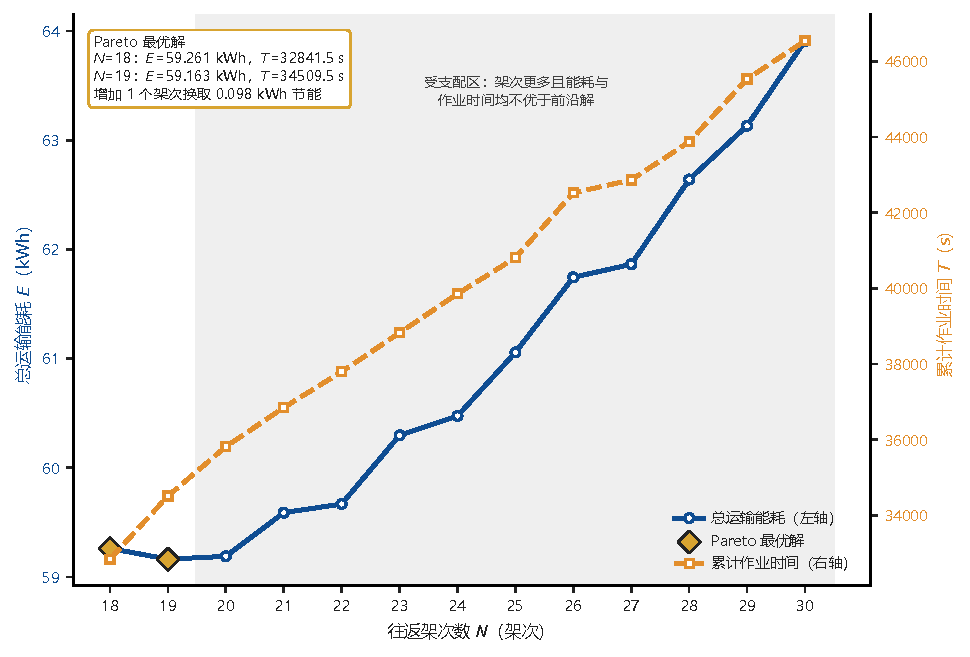
\includegraphics[width=0.88\textwidth]{../Q1/figures/fig_q1_tradeoff.pdf}
\caption{架次数、总运输能耗与累计作业时间的三指标权衡前沿}
\label{fig:q1tradeoff}
\end{figure}

蓝色实线为总运输能耗随架次数的变化，橙色虚线为累计作业时间，金色菱形标出真实 Pareto 最优解。前沿曲线呈先降后升的形态：架次数由 18 增至 19 时能耗由 59.261 kWh 降至 59.163 kWh，降幅仅 0.098 kWh 即 0.17\%，而累计作业时间增加 1668.0 s；架次数达到 20 及以上时能耗与作业时间同时上升，进入受支配区。因此本场景的真实 Pareto 架次数集合为 $\{18,19\}$，且应以最少架次数为首要目标，能耗为次要目标，作业时间随之自然优化。

返航安全余量的灵敏度结果如表~\ref{tab:q1sens} 所示。

\begin{table}[htbp]
\centering
\caption{返航安全余量对组批结果的影响}
\label{tab:q1sens}
\renewcommand\arraystretch{1.15}
\begin{tabular}{|c|c|c|c|}
  \hline
  返航安全余量 $\rho$ 区间 & 总架次数/架次 & 总能耗/kWh & 累计作业时间/s \\
  \hline
  0.10 -- 0.22 & 18 & 59.261 & 32841.5 \\
  \hline
  0.23 -- 0.26 & 19 & 61.214 & 34647.0 \\
  \hline
  0.27 -- 0.31 & 20 & 67.382 & 36671.6 \\
  \hline
  0.32 -- 0.33 & 20 & 71.926 -- 74.469 & 36908.2 -- 37008.1 \\
  \hline
  0.34 & 22 & 76.349 & 40582.4 \\
  \hline
  0.35 & 25 & 78.215 & 45621.0 \\
  \hline
  $\ge0.36$ & 不可行 & --- & --- \\
  \hline
\end{tabular}
\end{table}

余量由 0.22 提升至 0.23 时架次数首次跳变，此后呈阶梯式上升，至 0.35 时已达 25 架次、能耗 78.215 kWh，比基准方案多耗 31.98\%。$\rho$ 超过 0.3503 后模型不可行。该结果表明返航安全余量不能只从能耗角度放宽，必须与最重货箱的投递可行性联立考虑。

为了同时考察余量与需求规模的影响，本文在 $\rho$ 与需求缩放系数 $s$ 构成的二维网格上重算组批结果，得到 432 个网格点，其中 16 个点因最重货箱超出全部机型安全载荷而不可行，占比 3.7\%。可行点总架次数介于 16 与 27 之间，总运输能耗介于 51.761 kWh 与 91.610 kWh 之间。图~\ref{fig:sens} 给出响应面。

\begin{figure}[htbp]
\centering
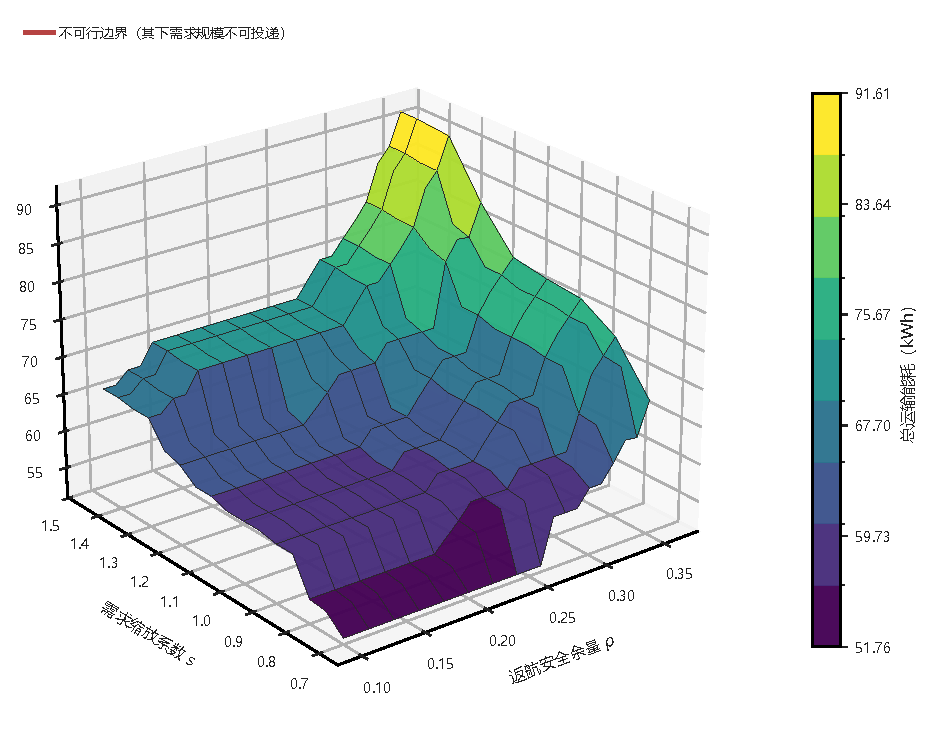
\includegraphics[width=0.86\textwidth]{../灵敏度分析/figures/fig_sens_surface.pdf}
\caption{返航安全余量与需求规模对总运输能耗的三维响应面}
\label{fig:sens}
\end{figure}

响应面显示总运输能耗关于余量与需求规模均单调递增，且需求规模的影响更为显著：在 $s=1$ 处余量由 0.10 升至 0.35 使能耗由 59.26 kWh 升至 76.35 kWh，而在 $\rho=0.10$ 处需求规模由 0.70 升至 1.45 使能耗由 51.76 kWh 升至 65.99 kWh。曲面存在明显台阶，台阶位置对应某服务区架次数增加的临界点，说明组批结果对余量的响应是分段常数而非连续变化。

本问所用能耗模型在原文意义上的展开见原理图提示词文件 手绘图/原理图-运输能耗构成.md。

\section{问题二模型建立与求解}

\subsection{问题分析与模型建立}
本问放开单点往返限制，允许一个架次访问多个服务区，并引入实体无人机、共享电池与时限约束。决策内容包括货箱组批、服务区访问顺序、运输机型、具体执行无人机、共享电池与各架次开始时刻，约束来自载荷与能量、机队与电池库存、充电周转以及首批截止时间与期望送达时间。

\subsubsection{多点多架次架次模型}
一个架次 $p$ 由三元组刻画：机型 $g(p)$、服务区有序序列 $\pi(p)=(i_1,\dots,i_m)$、以及各服务区的货箱集合。航线的载荷沿投送过程递减，设第 $k$ 段航段起点的剩余载荷为
\begin{equation}
q_k=\sum_{s=k}^{m}\sum_{b\in\mathcal{B}_{i_s}}m_b,
\label{eq:decpayload}
\end{equation}
即尚未投送的货箱质量之和。架次总能耗为各航段能耗之和，
\begin{equation}
E_p=\sum_{k=0}^{m}E_{i_k,i_{k+1}}^{g(p)}\!\left(q_k\right),\qquad i_0=i_{m+1}=O01,
\label{eq:sortieenergy}
\end{equation}
其中每段航段的几何量按式~\eqref{eq:segtime} 的口径重新计算，服务区之间航段的爬升高度以出发服务区地面海拔以上 30 m 为起点，与题面要求每次投送后重新爬升一致。架次可行性要求同时满足
\begin{equation}
\sum_{b\in p}m_b\le Q_{g(p)},\qquad
\sum_{b\in p}u_b\le V_{g(p)},\qquad
E_p\le\left(1-\rho_{g(p)}\right)E_{g(p)}^{use}.
\label{eq:sortiecons}
\end{equation}

\subsubsection{机队、电池与充电周转}
机型 $g$ 的实体无人机数量为 $K_g$，共享电池组数为 $B_g$，附件给定值分别为 A 型 4 架与 6 组、B 型 2 架与 4 组、C 型 2 架与 4 组。每架无人机在其排序序列中依次执行架次，架次 $p$ 的开始时刻为
\begin{equation}
t_p^{start}=\max\left\{\,t_u^{free},\;t_b^{ready}\,\right\},
\label{eq:starttime}
\end{equation}
其中 $t_u^{free}$ 为所分配无人机的空闲时刻，$t_b^{ready}$ 为所分配电池的就绪时刻。架次结束后电池的荷电状态为
\begin{equation}
s_p=1-\frac{E_p}{E_{g(p)}^{use}},
\label{eq:soc}
\end{equation}
电池再次就绪的时刻为 $t_p^{end}+t^{chg}(s_p)$，充电时间按以 0.90 为分界的两阶段等效模型计算，
\begin{equation}
t^{chg}(s)=
\begin{cases}
T^{full}\left[\,0.65\dfrac{0.90-s}{0.90}+0.35\,\right], & 0\le s<0.90,\\[2mm]
T^{full}\cdot0.35\dfrac{1-s}{0.10}, & 0.90\le s\le1 .
\end{cases}
\label{eq:charge}
\end{equation}
式~\eqref{eq:charge} 表明荷电状态低于 0.90 时按快充段的线性折算充电，高于 0.90 后转入慢充段，因此把电池用到很低的荷电状态会显著推迟其再次就绪时刻，这一非线性正是电池周转成为紧约束的原因。

\subsubsection{时限约束与四项指标}
首批保障货箱须在附件给定的首批截止时间前送达，构成硬约束；其余货箱的期望送达时间用于度量配送及时性，本文取按应急优先系数加权的总延误
\begin{equation}
D=\sum_{b}w_b\max\left(0,\;t_b-T_b^{exp}\right),
\label{eq:tardy}
\end{equation}
其中 $w_b$ 为货箱 $b$ 的应急优先系数，$t_b$ 为实际送达时刻，$T_b^{exp}$ 为期望送达时间。四项指标为加权总延误 $D$、全部任务完成时间 $M$、总运输能耗 $E$ 与往返架次数 $N$，其中完成时间按题面口径取所有运输无人机完成最后一个架次并返回 O01 的最晚时刻，
\begin{equation}
M=\max_{p}\left(t_p^{start}+\tau_{g(p)}\!\left(n_p\right)\right).
\label{eq:makespan}
\end{equation}

\subsubsection{分层构造与局部搜索}
本问的决策空间包含划分、排序、指派与排程四个层次，属于带时间窗与资源周转的异构多行程路径问题，精确求解在给定规模下不可行，故采用分层构造与局部搜索相结合的算法。构造阶段按截止时间把货箱分为三层，第一层为截止时间 3600 s 的首批货箱，第二层为截止时间 7200 s 与 10800 s 的首批货箱，第三层为其余物资。分层的作用是把首批货箱集中在少量架次中，使其能在第一波起飞窗口内出发，这是首批截止时间能否满足的结构性前提。每层内部按服务区聚合为投送单元，逐个开设新架次并尽量并入其他单元；机型选择按「加入后该机型架次数与实体无人机数之比」升序尝试，使机型负载自构造阶段就趋向均衡。

局部搜索在四个邻域上迭代：货箱迁移、同机型架次合并、机型替换与路线 2-opt，并以架次拆分作为补充邻域。接受准则为改进即接受，并以小概率接受劣解以避免早熟。由于同机型实体无人机数量有限，若某机型的架次数远超其无人机数，该机型会成为完成时间的瓶颈，因此搜索之后增加机型负载比再平衡过程：把瓶颈机型的架次整架次换型，或按冷机型能力拆成若干个冷机型架次，以目标函数为判据决定是否接受。

四项指标量纲不同，本文采用归一化加权和
\begin{equation}
J=w_1\frac{D}{D_0}+w_2\frac{M}{M_0}+w_3\frac{E}{E_0}+w_4\frac{N}{N_0}+\lambda\,\Phi,
\label{eq:q2obj}
\end{equation}
其中下标 $0$ 表示初始解的取值，$\Phi$ 为首批截止时间超时总量，$\lambda$ 取远大于其余权重系数的正数以保证硬约束优先。本文设置及时性优先、完成时间优先、能耗优先与均衡四套权重，并在统一的均衡权重下比较各方案，以避免用不同权重的目标值直接比较造成的口径错误。

求解流程见算法~\ref{alg:q2}。

\begin{algorithm}[H]
\caption{问题二分层构造与局部搜索算法}
\label{alg:q2}
\begin{algorithmic}[1]
\Require 货箱集合、机型参数、机队与电池库存、时限要求
\Ensure 组批方案、访问顺序、机型与执行无人机、电池与架次开始时刻
\State 按首批截止时间把货箱分为三层
\For{每个层}
  \State 按服务区聚合为投送单元，按紧急度排序
  \While{存在未分配单元}
    \State 取最紧急单元开设新架次，机型按负载比升序尝试
    \State 在不违反式~\eqref{eq:sortiecons} 的前提下并入其他单元
  \EndWhile
\EndFor
\State 合并同机型架次并对每个架次做路线 2-opt
\State 以式~\eqref{eq:q2obj} 为目标执行货箱迁移、合并、换型与拆分邻域搜索
\State 执行机型负载比再平衡，消除瓶颈机型
\State 按紧急度排序，用最早空闲无人机与最早就绪电池排定架次开始时刻
\State \Return 调度方案与四项指标
\end{algorithmic}
\end{algorithm}

\subsection{求解结果与分析}
四套权重方案的求解结果如表~\ref{tab:q2plans} 所示。

\begin{table}[htbp]
\centering
\caption{四套权重方案的指标结果}
\label{tab:q2plans}
\renewcommand\arraystretch{1.15}
\begin{tabular}{|c|c|c|c|c|c|}
  \hline
  权重方案 & 加权总延误 & 完成时间/s & 运输能耗/kWh & 架次数/架次 & 首批超时/s \\
  \hline
  及时性优先 & 157697.6 & 10032.4 & 95.647 & 32 & 0 \\
  \hline
  完成时间优先 & 221155.4 & 9743.2 & 95.406 & 32 & 0 \\
  \hline
  能耗优先 & 185230.1 & 10313.4 & 86.983 & 27 & 0 \\
  \hline
  均衡 & 166162.9 & 10366.7 & 87.547 & 29 & 0 \\
  \hline
\end{tabular}
\end{table}

四套方案的首批截止时间超时均为零，说明分层构造有效保证了硬约束。在统一的均衡权重下比较，能耗优先方案的目标值最小，故以其为主方案。该方案含 27 个运输架次、总运输能耗 86.983 kWh、全部任务完成时间 10313.4 s 即 2.865 h。图~\ref{fig:q2metrics} 以归一化矩阵给出四套方案在四项指标上的相对表现。

\begin{figure}[htbp]
\centering
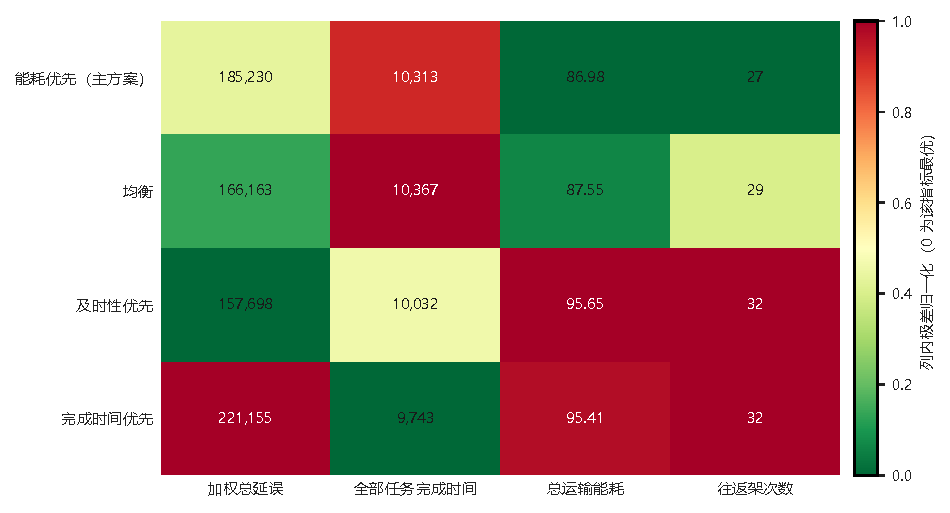
\includegraphics[width=0.86\textwidth]{../Q2/figures/fig_q2_plan_metrics.pdf}
\caption{四套权重方案在四项指标上的归一化表现矩阵}
\label{fig:q2metrics}
\end{figure}

矩阵按列做极差归一化，绿色表示该指标最优、红色表示最差，格内数字为原始取值。四套方案在四个指标列上各自取得至少一个最优值，且没有任何一套在所有列上都不劣于其他方案，因此四套方案互为非受支配，构成四指标 Pareto 集。能耗优先方案在能耗与架次数两列最优，及时性优先方案在加权总延误列最优，完成时间优先方案在完成时间列最优。这一结构说明四项指标之间存在实质冲突：能耗优先方案比及时性优先方案少耗 8.66 kWh，代价是加权总延误增加 27532.5；比完成时间优先方案少耗 8.42 kWh，代价是完成时间增加 570.2 s。

图~\ref{fig:q2delivery} 给出主方案的逐服务区送达时刻分布。

\begin{figure}[htbp]
\centering
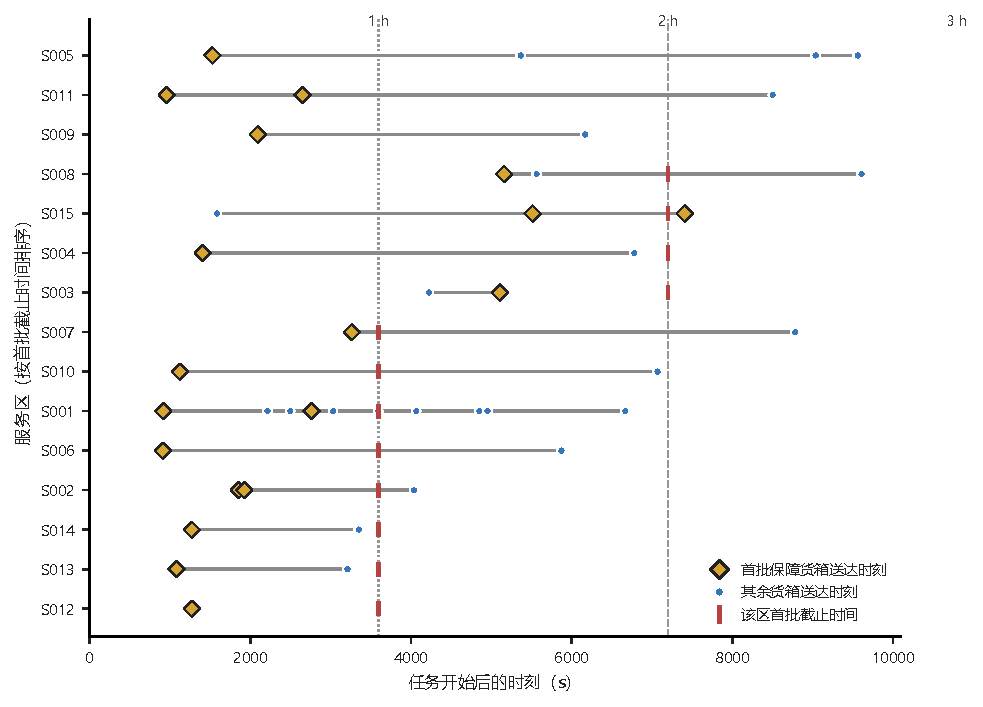
\includegraphics[width=0.88\textwidth]{../Q2/figures/fig_q2_delivery_timeline.pdf}
\caption{主方案逐服务区送达时刻相对首批截止档位的分布}
\label{fig:q2delivery}
\end{figure}

图中纵轴为服务区并按首批截止时间升序排列，横向灰线为该区全部货箱的送达时间范围，金色菱形为首批保障货箱的送达时刻，蓝色圆点为其余货箱，红色竖线为该区首批截止时间，三条灰色虚线为 1 h、2 h 与 3 h 档位。全部金色菱形均位于对应红色竖线左侧，即首批保障货箱全部在截止时间前送达，其中最早的 S012 首批货箱在 1090 s 左右完成投送。S001 因需求最大，其货箱送达时刻跨越 900 s 至 6000 s 的较宽区间。

图~\ref{fig:q2load} 给出各机型架次载荷利用率的分布。

\begin{figure}[htbp]
\centering
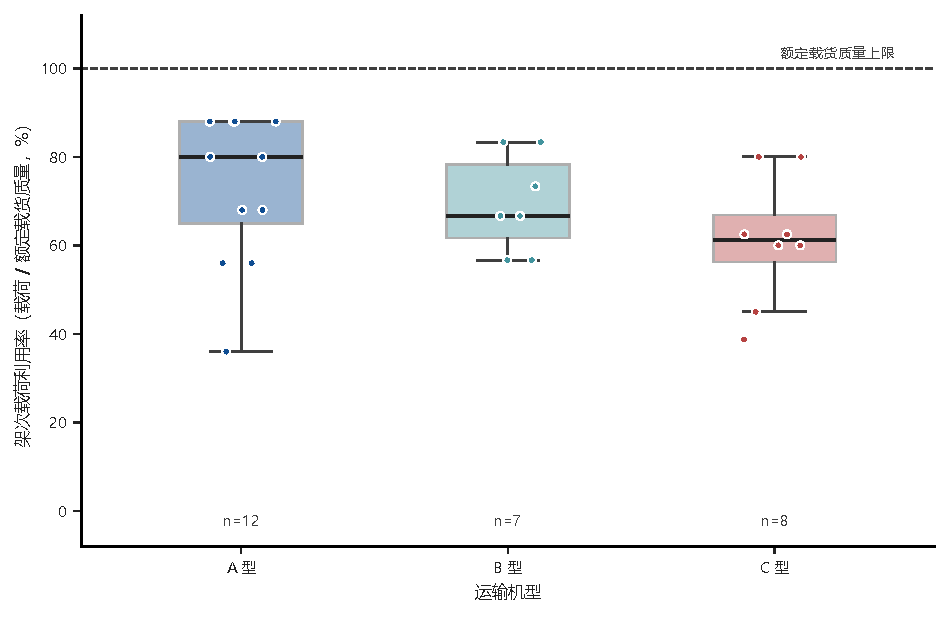
\includegraphics[width=0.86\textwidth]{../Q2/figures/fig_q2_load_utilization.pdf}
\caption{各机型架次载荷利用率的分布}
\label{fig:q2load}
\end{figure}

箱线图叠加原始散点，横轴为机型，纵轴为架次载荷与额定载货质量之比。A 型中位数约 80\%，四分位区间 65\% 至 87\%；B 型中位数约 66\%，区间 58\% 至 78\%；C 型中位数约 62\%，区间 55\% 至 67\%，且存在 39\% 的低值。C 型利用率最低的原因是其额定载货质量 80 kg 远大于单个服务区的需求规模，而 C 型又因容量优势被用于承运多个服务区的合并载荷，在能量约束下无法总是装满。A 型利用率高而架次数少，说明其在本场景中承担的是高频率小批量投送。

主方案的资源使用情况如表~\ref{tab:q2resource} 所示。

\begin{table}[htbp]
\centering
\caption{主方案的机队与共享电池使用情况}
\label{tab:q2resource}
\renewcommand\arraystretch{1.15}
\begin{tabular}{|c|c|c|c|c|}
  \hline
  机型 & 实体无人机/架 & 承担架次/架次 & 共享电池/组 & 电池最大就绪时刻/s \\
  \hline
  A 型 & 4 & 12 & 6 & 约 8500 \\
  \hline
  B 型 & 2 & 7 & 4 & 约 9200 \\
  \hline
  C 型 & 2 & 8 & 4 & 约 10400 \\
  \hline
\end{tabular}
\end{table}

资源可行性核对结果如下：实体无人机编号全部落在机队范围内，共享电池使用组数不超过库存，全部架次的载质量与装载体积均不超限，最紧架次的能耗占返航上限比例小于 1，80 个货箱全部被且仅被安排一次，各架次内货箱归属服务区与访问序列一致。

本问调度模型的结构与层间耦合关系见 手绘图/机制图-中继通信保障.md 所描述的中继保障机制，该机制在问题三中被正式纳入模型。

\section{问题三模型建立与求解}

\subsection{问题分析与模型建立}
本问在问题二的调度框架上增加连续通信约束。运输无人机在爬升、巡航、下降及物资投送阶段均应保持连续通信，直连不可用时须由一架中继无人机同时提供接入链路与回传链路。图~\ref{fig:framework} 给出运输层、通信层与资源层的三层协同框架。

\begin{figure}[htbp]
\centering
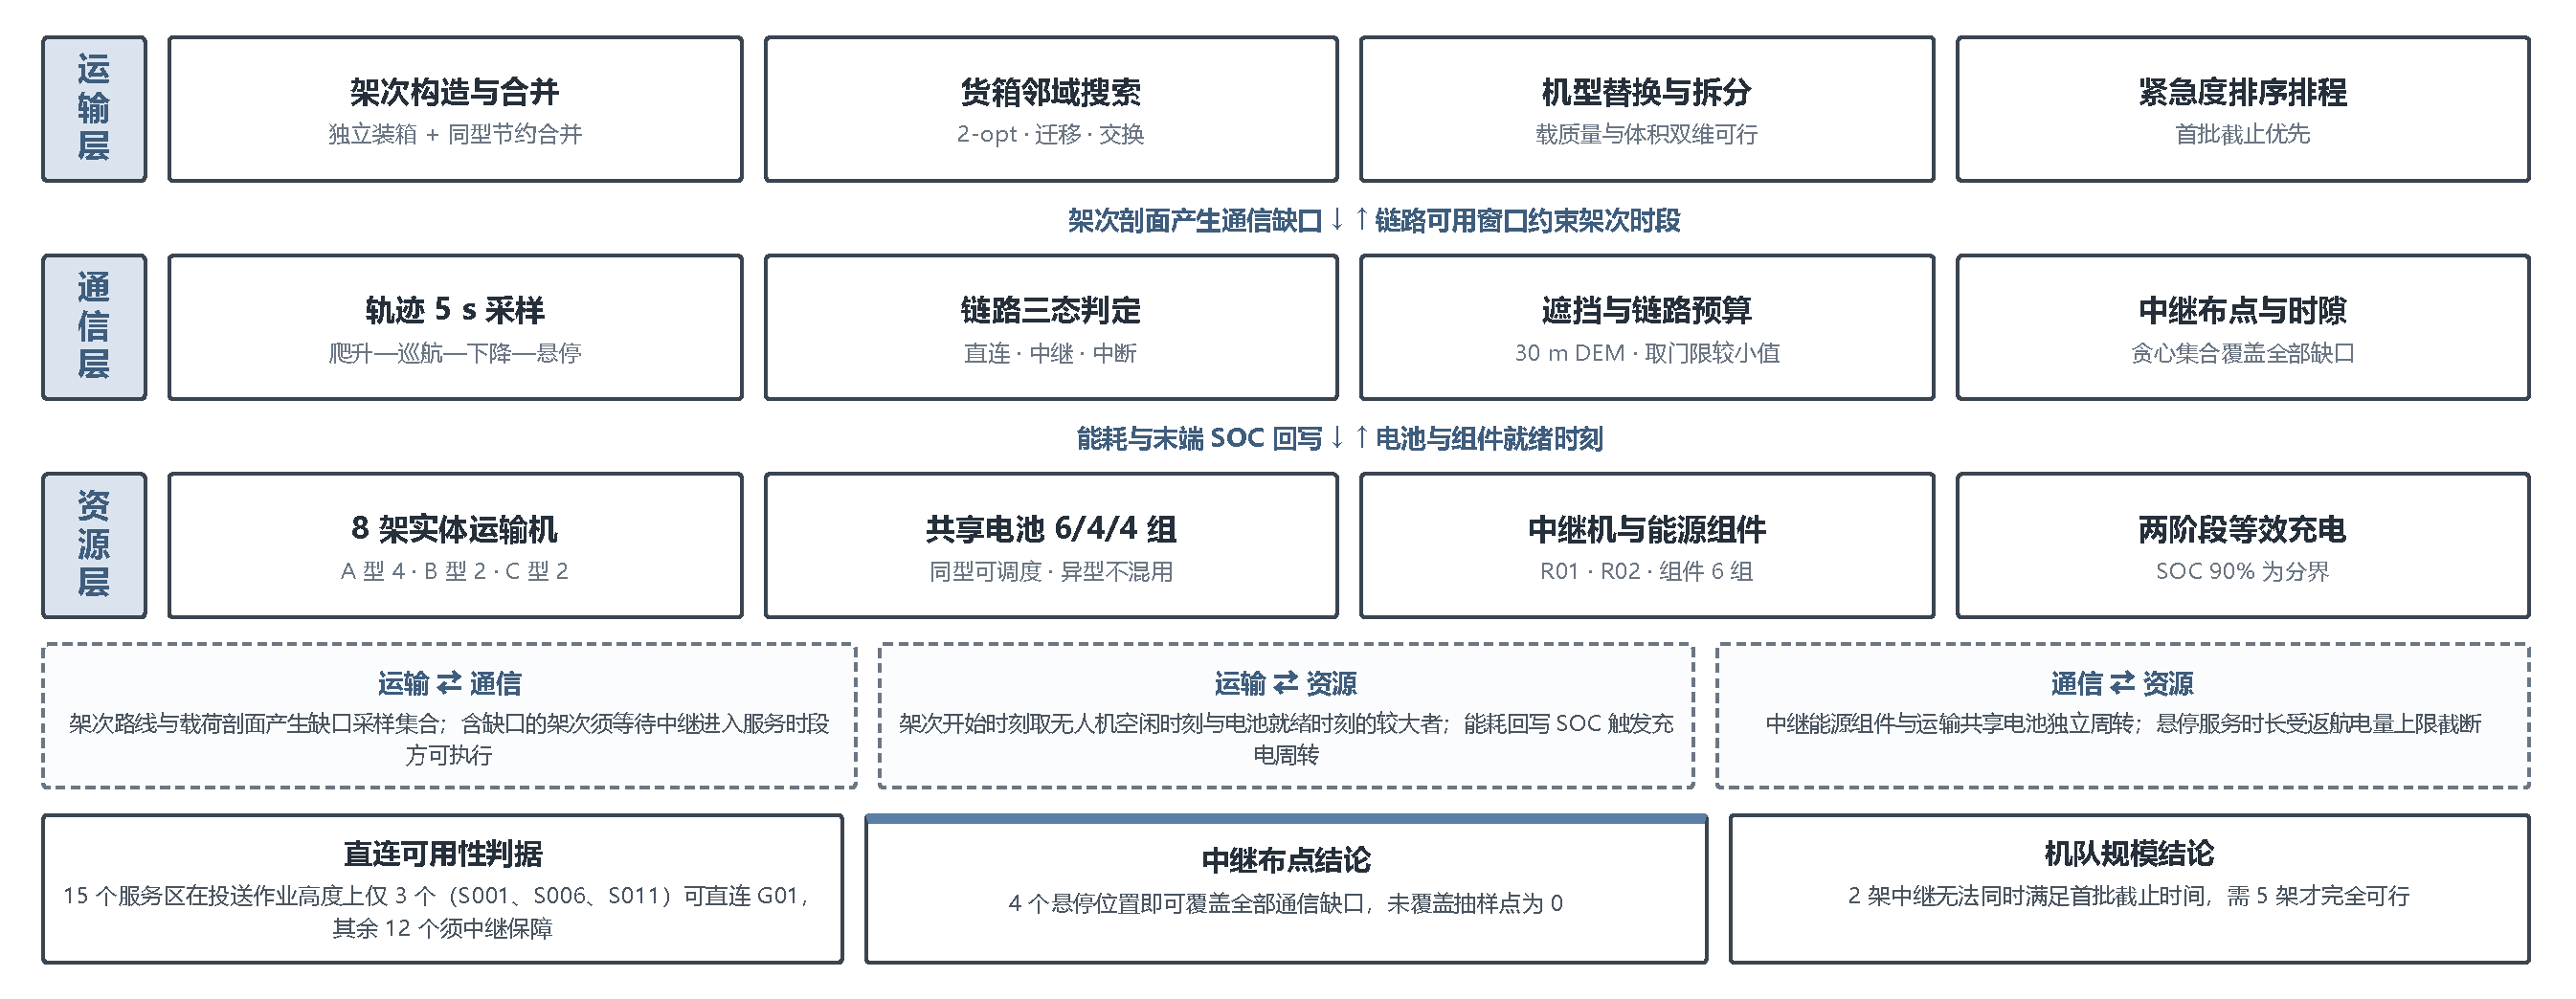
\includegraphics[width=\textwidth]{../手绘图/运输中继协同调度框架图.pdf}
\caption{运输层、通信层与资源层的三层协同框架与层间信息流}
\label{fig:framework}
\end{figure}

\subsubsection{运输轨迹采样}
为核验连续通信，需要把离散的架次展开为时序轨迹。对架次 $p$ 的每个航段 $i\to j$，按爬升、巡航与下降三个阶段分别以固定时间步采样三维位置，并在服务区投送期间按交接时长采样悬停位置。记采样点集合为 $\mathcal{P}_p$，采样步长取 5 s。轨迹展开使通信状态从「某架次是否可通信」细化为「架次在每一时刻是否可通信」，这是连续通信约束能够被逐点核验的前提。

\subsubsection{通信链路状态判断}
按题面附录 3 的口径，任意两个通信端点之间的地形遮挡变量由三维位置与 30 米 DEM 决定，
\begin{equation}
b_{ij}(t)=
\begin{cases}
1, & \text{端点 }i\text{ 与 }j\text{ 之间存在地形遮挡},\\
0, & \text{不存在地形遮挡}.
\end{cases}
\label{eq:block}
\end{equation}
接收门限由接收灵敏度与衰落裕量共同确定，$P_{th}^{b}=P_{sens}^{b}+M^{b}$。对通信方向 $a\to b$，最大允许总传播损耗为
\begin{equation}
L_{\max}^{a\to b}=P_t^{a}+G_t^{a}+G_r^{b}-L_{sys}-P_{th}^{b},
\label{eq:linkbudget}
\end{equation}
其中 $P_t$、$G_t$、$G_r$ 分别为发射功率、发射天线增益与接收天线增益，$L_{sys}$ 为系统损耗。由于运输控制与状态回传均需通信保障，主体 $a$ 与 $b$ 之间按双向链路判断，门限取两个方向最大允许损耗中的较小值，
\begin{equation}
L_{\max}^{a\leftrightarrow b}=\min\left(L_{\max}^{a\to b},\;L_{\max}^{b\to a}\right).
\label{eq:bidir}
\end{equation}
自由空间传播损耗按
\begin{equation}
L_{FSPL,ij}(t)=32.45+20\log_{10}f+20\log_{10}D_{ij}(t)
\label{eq:fspl}
\end{equation}
计算，其中载波频率 $f$ 以 MHz 计、三维直线距离 $D_{ij}$ 以 km 计。计入地形遮挡后的总传播损耗为
\begin{equation}
L_{path,ij}(t)=L_{FSPL,ij}(t)+L^{obs}b_{ij}(t),
\label{eq:pathloss}
\end{equation}
链路可用性为
\begin{equation}
A_{ij}(t)=
\begin{cases}
1, & L_{path,ij}(t)\le L_{\max}^{i\leftrightarrow j},\\
0, & L_{path,ij}(t)>L_{\max}^{i\leftrightarrow j}.
\end{cases}
\label{eq:avail}
\end{equation}
运输无人机在任一时刻的通信状态按三态规则确定：与固定网关链路可用时记为直连状态；直连不可用但运输无人机与中继的接入链路和中继与网关的回传链路同时可用时记为中继状态；其余情况记为通信中断状态。采用中继服务时两段链路必须在同一时刻同时可用，且每架运输无人机在任一时刻只能由网关或一架中继提供通信保障。

\subsubsection{中继悬停位置与架次模型}
中继无人机由 O01 出发，到达悬停位置并完成建链后提供通信服务，服务结束后返回 O01。悬停位置 $(\lambda_h,\varphi_h)$ 须位于 DEM 覆盖范围内，悬停离地高度 $h_h$ 不超过附件规定上限 300 m，故悬停海拔为
\begin{equation}
z_h=z_{ground}\!\left(\lambda_h,\varphi_h\right)+h_h .
\label{eq:hoveralt}
\end{equation}
中继往返悬停位置的时间按与运输航段相同的爬升、巡航与下降规则计算，计划巡航海拔取沿途 DEM 最高地面高程以上 50 m。中继架次能耗由飞行能耗与通信服务能耗两部分构成，
\begin{equation}
E^{R}=E^{R}_{flight}+E^{R}_{service},
\label{eq:relayenergy}
\end{equation}
其中飞行能耗中水平巡航部分按巡航功率与巡航时间计算，
\begin{equation}
E^{R}_{cruise}=P^{c}_{R}\cdot\frac{d_{O01,h}}{v^{c}_{R}}\Big/3600,
\qquad
E^{R}_{climb}=\frac{m^{R}_{takeoff}\,\rho_e\left(h^{+}_{out}+h^{+}_{back}\right)}{3.6\times10^{6}\eta^{\uparrow}_{R}},
\label{eq:relayflight}
\end{equation}
通信服务能耗由悬停功率与通信附加功率共同确定，
\begin{equation}
E^{R}_{service}=\left(P^{hover}_{R}+P^{comm}_{R}\right)\cdot\frac{\tau_{service}}{3600},
\label{eq:relayservice}
\end{equation}
并须满足返航电量要求 $E^{R}\le\left(1-\rho_R\right)E^{comp}_{R}$。由式~\eqref{eq:relayservice} 与能量上限可解出单架次最大连续服务时长
\begin{equation}
\tau^{max}_{service}=\frac{\left(1-\rho_R\right)E^{comp}_{R}-E^{R}_{flight}}{P^{hover}_{R}+P^{comm}_{R}}\times3600 .
\label{eq:svcmax}
\end{equation}
代入附件参数可得单架次最大连续服务时长约为 2.2 h，这一上限直接决定了中继机队规模的下界。

\subsubsection{中继布点与联合调度}
把全部通信缺口采样点作为待覆盖集合，在 DEM 覆盖范围内构造候选悬停位置，包括 15 个服务区上空与区域内的高地形点，每个候选位置配以若干悬停离地高度。以候选位置对缺口点的覆盖关系作贪心集合覆盖，每次选择覆盖未覆盖点最多的候选，直至缺口全部被覆盖。

在布点确定后，每个悬停位置对应一个必须提供服务的时段区间，其上下界为该位置所覆盖缺口采样时刻的最小值与最大值。中继架次按所服务运输架次的紧急度排序后依次分配到中继无人机与能源组件，开始时刻取无人机空闲时刻与组件就绪时刻的较大者。含通信缺口的运输架次须等待覆盖其自身缺口的中继进入服务时段，故运输时刻与中继窗口互为因果，本文采用单次口径确定：先按问题二的运输时刻确定中继服务窗口，再把运输架次推迟至所属中继就绪。反复重排会使推迟与窗口拉长形成正反馈，故不作二次重排。

\subsection{求解结果与分析}
链路门限计算结果为运输无人机与网关之间 122.0 dB，运输无人机与中继接入端之间 116.0 dB，中继回传端与网关之间 126.0 dB。按 5 s 步长对 27 个运输架次展开轨迹，共得 9022 个采样点，其中直连不可用的缺口点 3536 个，占 39.19\%。

缺口在服务区之间的分布并不均匀。按最近服务区归集后，S002 有 481 个缺口点、S008 有 445 个、S005 有 435 个，而 S001 与 S011 各仅 2 个。图~\ref{fig:q3margin} 给出 15 个服务区在投送作业高度上的直连链路余量分布，以及运输无人机与中继接入链路的余量分布。

\begin{figure}[htbp]
\centering
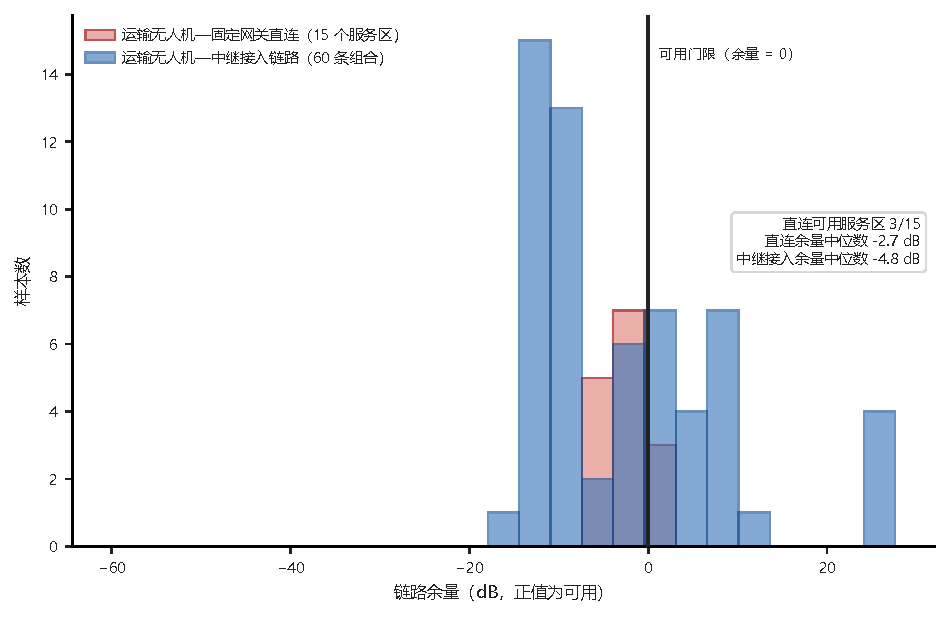
\includegraphics[width=0.86\textwidth]{../Q3/figures/fig_q3_link_margin.pdf}
\caption{直连链路与中继接入链路的余量分布}
\label{fig:q3margin}
\end{figure}

余量定义为门限与实际总损耗之差，正值表示链路可用。15 个服务区在作业高度上仅 3 个的直连余量为正，直连余量中位数为 $-2.7$ dB；中继接入链路的余量中位数为 $-4.8$ dB，但在 60 条组合中有 29 条为正。可见在投送作业高度上，山区地形遮挡使直连通信在多数服务区不可用，空中中继是恢复通信的必要手段而非可选增强。

贪心集合覆盖选出的 4 个悬停位置均取悬停离地高度 300 m，覆盖全部缺口抽样点，未覆盖抽样点为 0。图~\ref{fig:q3layout} 给出运输航迹、中继悬停位置及其到网关的回传链路。

\begin{figure}[htbp]
\centering
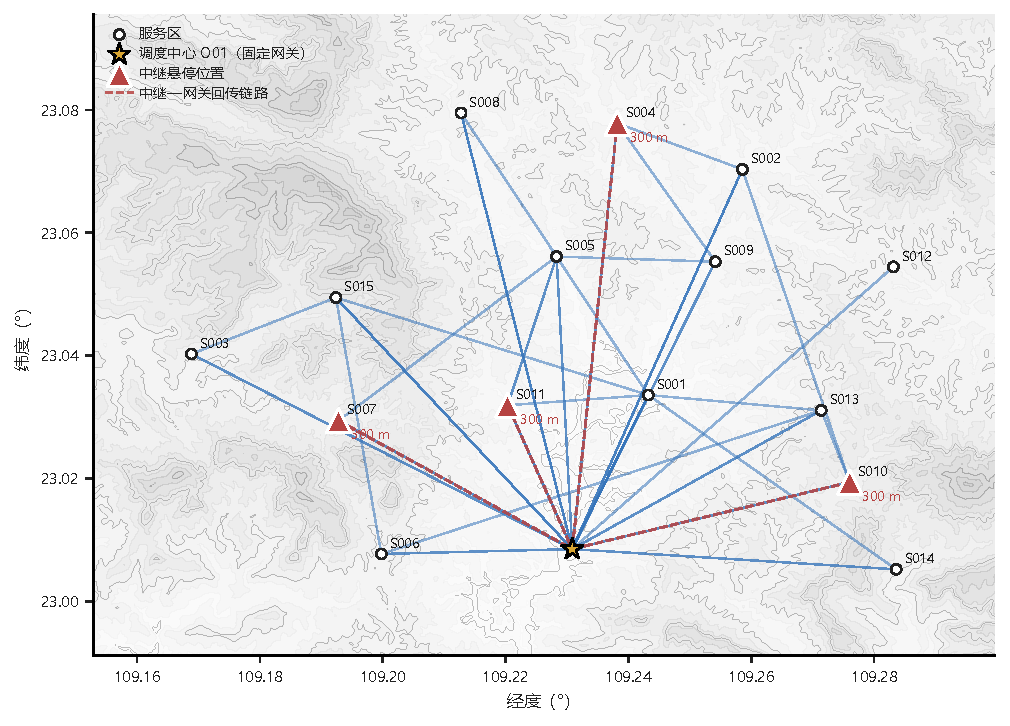
\includegraphics[width=0.92\textwidth]{../Q3/figures/fig_q3_relay_layout.pdf}
\caption{运输航迹、中继悬停位置与回传链路}
\label{fig:q3layout}
\end{figure}

四个悬停位置分别位于 S011、S004、S007 与 S010 上空，海拔介于 473.1 m 与 627.1 m 之间，往返飞行时间介于 472.2 s 与 1195.2 s 之间。中继在区域中部与东部各设一处，覆盖中央服务区群与东北服务区群；西部与东南部各设一处，覆盖西部山区与东南丘陵。四处悬停位置的回传链路均指向调度中心 O01，链路走向跨越的地形起伏在图中的 DEM 灰阶背景上可直接读出。

中继架次与联合调度结果如表~\ref{tab:q3missions} 所示。

\begin{table}[htbp]
\centering
\caption{中继架次安排}
\label{tab:q3missions}
\renewcommand\arraystretch{1.15}
\begin{tabular}{|Y{0.09}|W{0.20}|Y{0.135}|Y{0.135}|Y{0.135}|Y{0.125}|Y{0.155}|}
  \hline
  中继 & 悬停位置 & 建链完成/s & 服务结束/s & 服务时长/s & 能耗/kWh & 末端荷电状态 \\
  \hline
  R01 & S011 上空 & 439.2 & 5128.1 & 4688.9 & 1.5074 & 0.529 \\
  \hline
  R02 & S010 上空 & 604.8 & 6938.8 & 6334.0 & 2.0643 & 0.355 \\
  \hline
  R01 & S004 上空 & 6467.2 & 10807.4 & 4340.2 & 1.5159 & 0.526 \\
  \hline
  R02 & S007 上空 & 8267.3 & 15801.7 & 7534.4 & 2.4329 & 0.240 \\
  \hline
  R01 & S011 上空 & 12155.8 & 16844.7 & 4688.9 & 1.5074 & 0.529 \\
  \hline
  R02 & S004 上空 & 17328.1 & 21668.3 & 4340.2 & 1.5159 & 0.526 \\
  \hline
\end{tabular}
\end{table}

6 个中继架次使用 2 架中继无人机与全部 6 组能源组件，末端荷电状态最低为 0.240，高于 0.20 的返航电量下限。中继总能耗 10.544 kWh，运输总能耗 86.983 kWh，联合总能耗 97.527 kWh。

由于运输时刻与中继窗口相互耦合，本文给出两种口径的对照。通信优先口径下运输架次推迟至所属中继就绪，通信缺口采样点全部被覆盖，未保障点为 0，但首批截止时间超时合计 76014.2 s，联合任务完成时间 22577.5 s。时限优先口径下保持问题二的运输时刻不变、只让中继去匹配运输时刻，首批截止时间超时为零，但有 796 个采样点未被保障，占 8.8\%，联合任务完成时间同为 22577.5 s。两种口径的对照说明在给定 2 架中继的条件下，全程通信保障与首批时限满足无法同时实现。

为确定所需的中继机队规模，本文在其余条件不变的前提下改变中继无人机数量重算联合调度，完整结果见附录表~\ref{tab:appq3b}。



中继无人机数量由 2 架增至 4 架时，首批超时由 76014.2 s 单调降至 1380.8 s，同时通信缺口采样点始终为 0，即首批时限逐步改善而通信保障未被削弱。增至 5 架时首批超时降为零，但未保障点由 0 升至 414 个；增至 6 架时首批超时仍为零而未保障点进一步升至 808 个。其原因是中继架数增加使运输架次得以更早起飞，运输轨迹在时间轴上被压缩，部分缺口时刻移出了按原运输时刻确定的中继服务窗口，因而出现「时限满足而个别时刻通信未被覆盖」的新形态。

由此可见，在 2 至 6 架中继范围内，首批截止时间全部满足与通信缺口全部覆盖无法同时达成：4 架以下通信覆盖完整但首批超时，5 架以上首批时限满足但存在数百个未保障采样点。若要求两者同时成立，则所需中继资源超过本文扫描的 6 架上界。该结论与式~\eqref{eq:svcmax} 给出的单架次服务时长上限一致：4 个悬停位置的服务窗口跨度合计约 3.0$\times$10$^4$ s，而单架中继在完成时间窗口内的可用服务时长约为 0.8$\times$10$^4$ s，两者相除给出所需并发架数的量级下界，但由于服务窗口必须与运输时刻严格对齐，实际所需架数还要更高。这一资源紧张状况正是问题四需要按任务组独立核算资源缺口的原因。

本问的联合调度在完成时间上比问题二增加 12264.1 s，能耗增加 10.544 kWh，代价来自通信保障环节，属于题目要求下不可避免的代价。

\section{问题四模型建立与求解}

\subsection{问题分析与模型建立}
本问在问题三方案的基础上研究任务分区与资源配置。图~\ref{fig:q4flow} 给出分区、独立核算与冗余缺口评估的判断流程。

\begin{figure}[htbp]
\centering
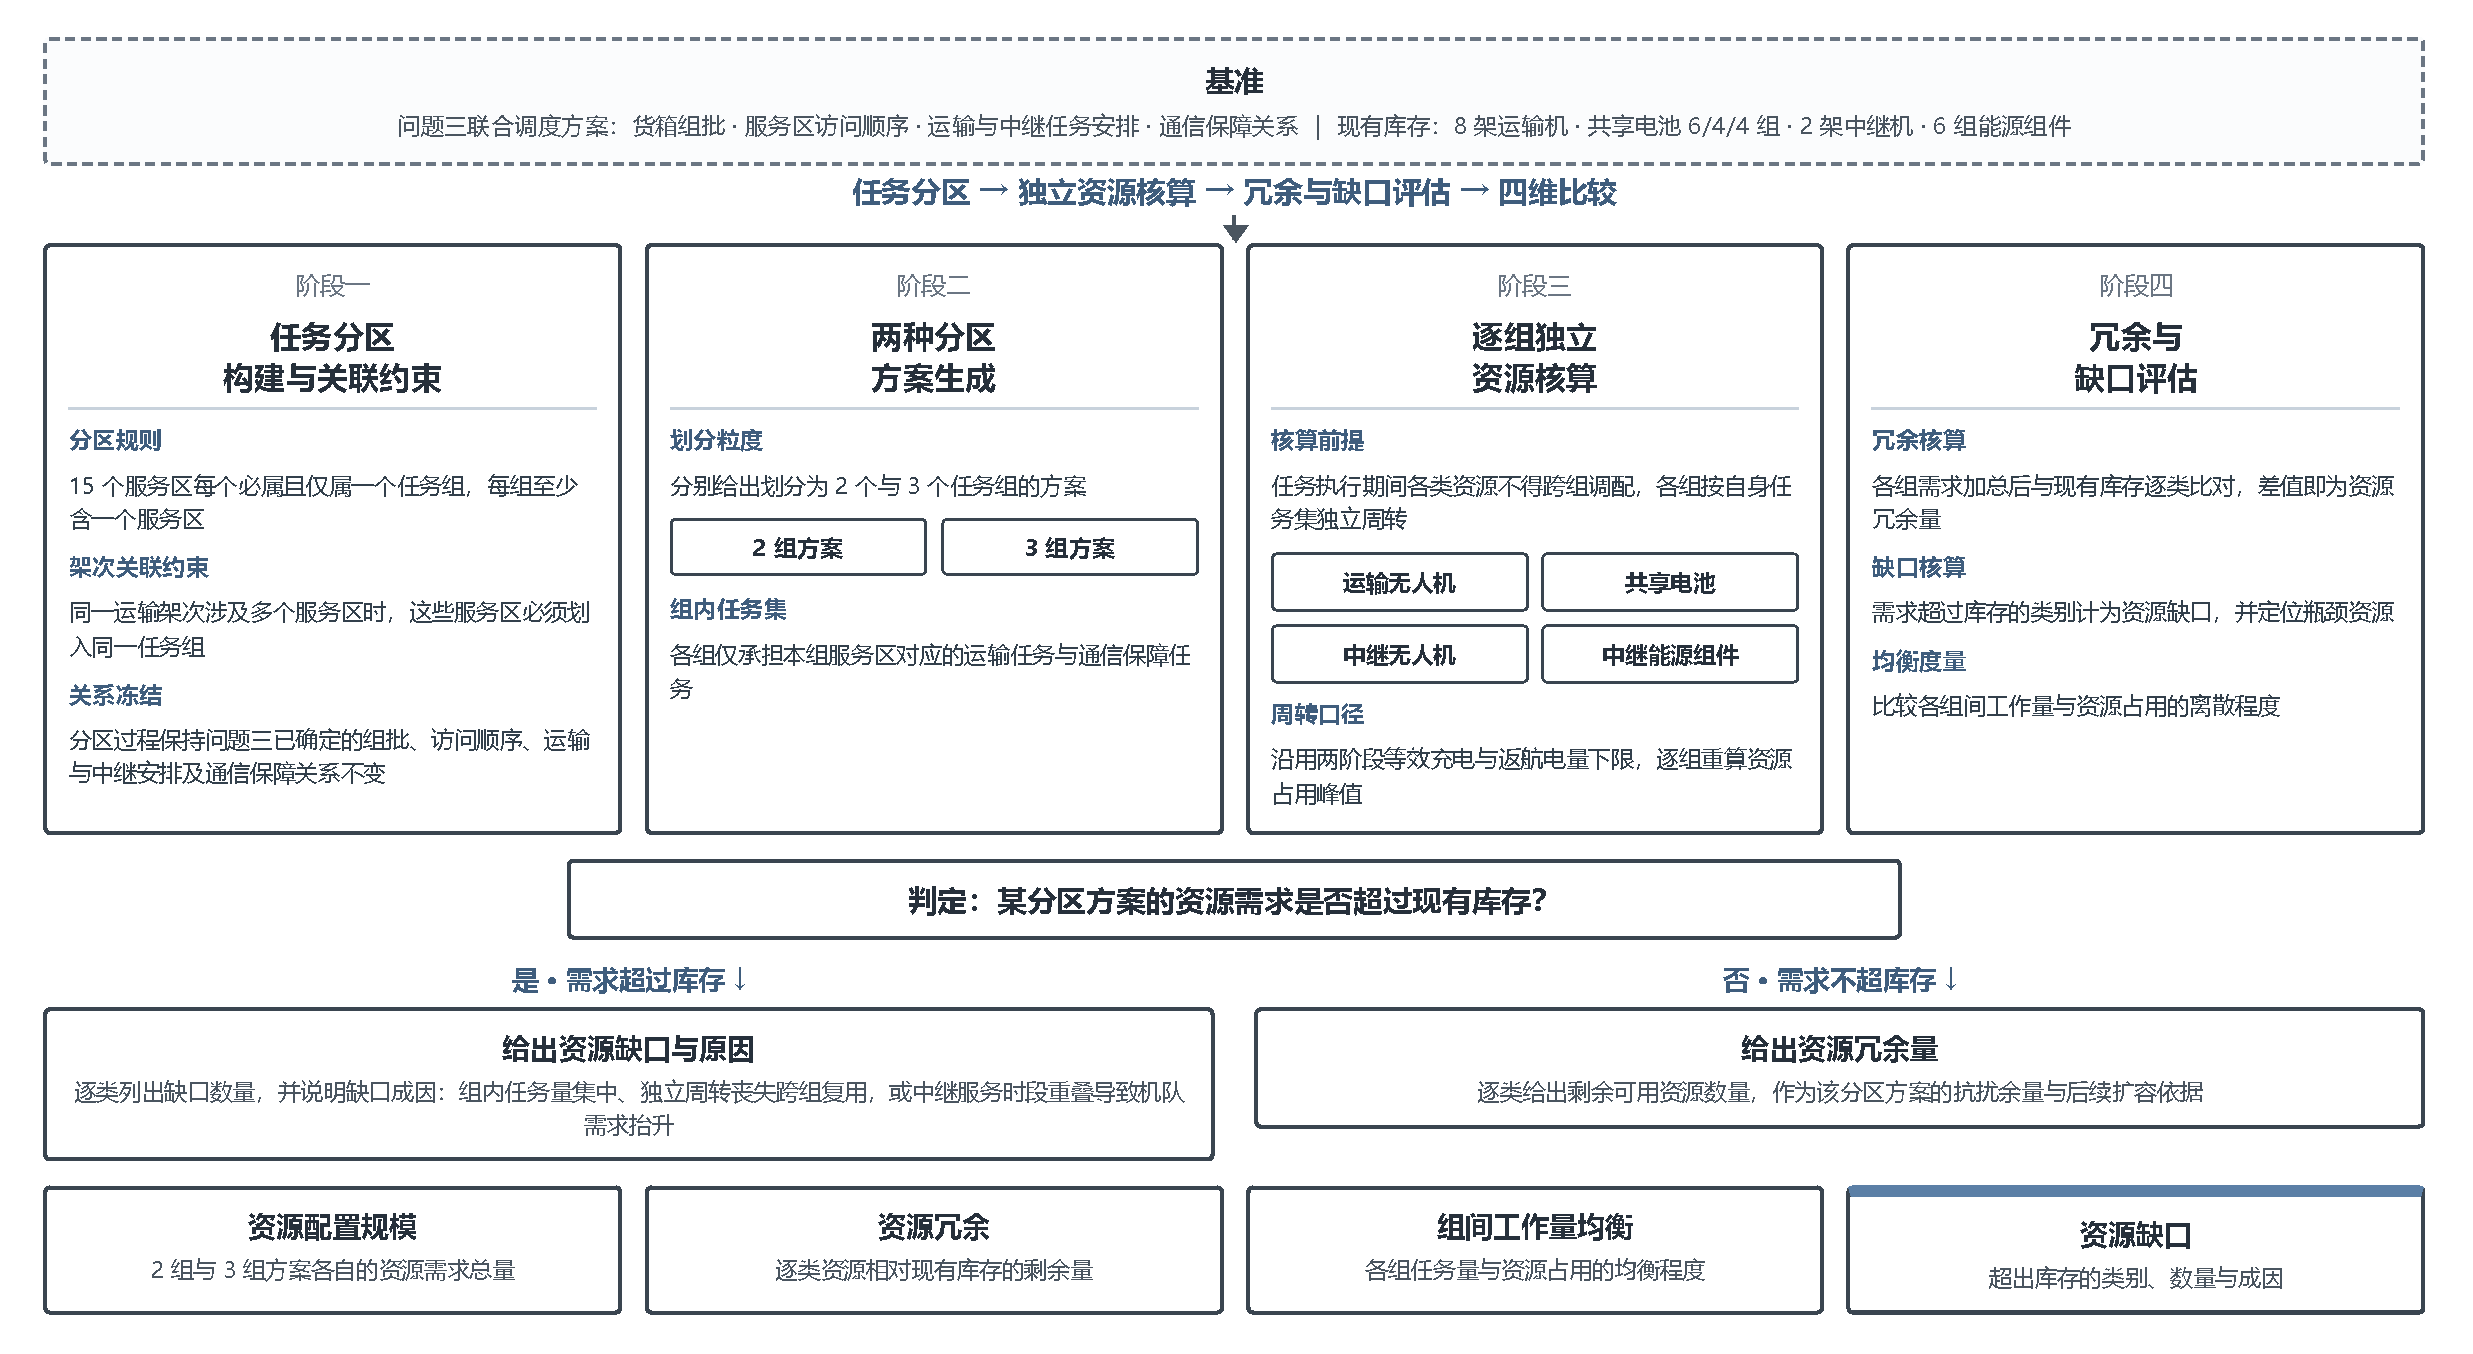
\includegraphics[width=\textwidth]{../手绘图/任务分区评估流程图.pdf}
\caption{任务分区、逐组独立资源核算与冗余缺口评估流程}
\label{fig:q4flow}
\end{figure}

\subsubsection{同架次必须同组的关系图}
题面要求若同一运输架次同时涉及多个服务区，则这些服务区应划入同一任务组。以服务区为点、以同一架次内相邻服务区对为边构建关系图，则每个连通分量构成一个不可拆分的基本单元。设关系图有 $c$ 个连通分量，则任务组数不得超过 $c$。

在问题三的 27 个运输架次中共有 17 条相邻关系，连通分量为 2 个：一个分量含 14 个服务区，另一个分量仅含 S012。S012 之所以独立，是因为在问题三方案中它仅由单服务区架次承运。该结果表明，若严格保持问题三的架次结构不变，2 组分区只能取「14 个服务区」与「S012」这一极端不均衡的划分，3 组分区则不存在可行划分。

题面同时规定各任务组仅承担本组服务区对应的运输与通信保障任务，并分别核算独立执行所需的资源数量，这一要求本身就意味着各组需要按同一套规则重新组批。因此本文采用分区后组内重新组批的口径：货箱归属、服务区访问顺序、能耗与通信判断规则保持不变，跨组架次按任务组拆分为组内架次。在该口径下，组内架次只覆盖本组服务区，同架次必须同组的约束自动满足。

\subsubsection{任务分区构造}
分区需同时考虑组间工作量均衡与组内空间紧凑。以全部服务区的加权质心为极点，计算各服务区绕质心的极角并按极角排序，在排序序列上取 $k-1$ 个切点将序列切成 $k$ 段。切点组合共 $\binom{14}{k-1}$ 种，对每种组合计算代价
\begin{equation}
\Psi=\frac{\max_k W_k-\min_k W_k}{\bar{W}}+0.35\cdot\frac{\sum_k S_k}{\bar{S}},
\label{eq:partcost}
\end{equation}
其中 $W_k$ 为第 $k$ 组的货箱总质量，$S_k$ 为该组服务区经纬度跨度的较大值，$\bar{W}$ 与 $\bar{S}$ 为相应均值。第一项度量组间工作量不均衡，第二项度量组内空间跨度，取最小代价的切分作为分区方案。采用角度扫描而非一般聚类的原因是该方式保证分区在空间上连贯，便于各组独立执行时按地理方向组织航线。

\subsubsection{组内独立资源核算}
对每个任务组独立重跑装箱、同机型合并与路线优化，得到组内运输架次集合。运输无人机需求按满足全部首批截止时间所需的最少架数核定：对给定机型的组内架次集合，从 1 架起逐一试算，模拟按最早空闲无人机与最早就绪电池排定架次并计入充电周转，取首批超时为零的最小架数。共享电池需求在所需无人机数下按同样方式核定，取使完成时间不超过该机型最短可行完成时间的最小电池组数。

中继需求按服务区间的最大重叠数核定。对每个选出的悬停位置计算其必须提供服务的时段区间，中继无人机数等于这些区间在时间上的最大重叠数，即区间图着色数；中继能源组件数等于计入充电周转后的资源占用区间的最大重叠数。该口径直接给出独立执行所需的最小并发资源量，且不依赖运输时刻的重排。

\subsection{求解结果与分析}
两种分区的划分结果如表~\ref{tab:q4partition} 所示。

\begin{table}[htbp]
\centering
\caption{2 组与 3 组分区的任务组构成}
\label{tab:q4partition}
\renewcommand\arraystretch{1.15}
\begin{tabular}{|Y{0.10}|Y{0.11}|W{0.51}|Y{0.14}|Y{0.14}|}
  \hline
  分区 & 任务组 & 服务区 & 货箱数/箱 & 需求质量/kg \\
  \hline
  \multirow{2}{*}{2 组} & 组 1 & S001、S003、S006、S007、S011、S014 & 40 & 389 \\
  \cline{2-5}
   & 组 2 & S002、S004、S005、S008、S009、S010、S012、S013、S015 & 40 & 369 \\
  \hline
  \multirow{3}{*}{3 组} & 组 1 & S003、S006、S007、S011 & 22 & 210 \\
  \cline{2-5}
   & 组 2 & S001、S009、S010、S012、S013、S014 & 30 & 279 \\
  \cline{2-5}
   & 组 3 & S002、S004、S005、S008、S015 & 28 & 269 \\
  \hline
\end{tabular}
\end{table}

2 组分区把服务区按东西向分成两个质量接近的任务组，组间质量分别为 389 kg 与 369 kg。3 组分区按西北、中部与东北三个方向切分，质量分别为 210 kg、279 kg 与 269 kg。图~\ref{fig:q4partition} 给出同架次必须同组关系、两种分区的归属以及资源配置对比。

\begin{figure}[htbp]
\centering
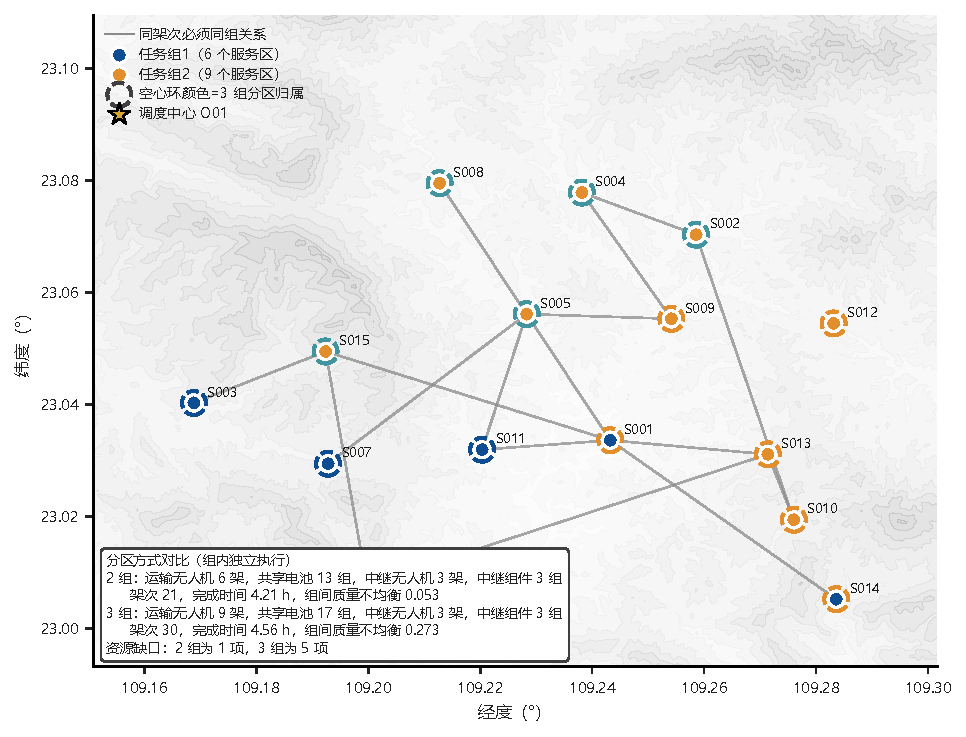
\includegraphics[width=0.92\textwidth]{../Q4/figures/fig_q4_partition.pdf}
\caption{同架次必须同组关系、两种分区归属与资源配置对比}
\label{fig:q4partition}
\end{figure}

图中灰色连线为同架次必须同组关系，实心圆颜色表示 2 组分区的归属，空心环颜色表示 3 组分区的归属，左下角文本框给出两种分区的资源需求与缺口数量。可以看出同架次关系把 14 个服务区连成一片，仅 S012 因全部由单区架次承运而孤立，这印证了前文关于连通分量的分析。

两种分区的独立资源核算结果如表~\ref{tab:q4compare} 所示。

\begin{table}[htbp]
\centering
\caption{2 组与 3 组分区在四个维度上的对比}
\label{tab:q4compare}
\renewcommand\arraystretch{1.15}
\begin{tabular}{|Y{0.10}|Y{0.15}|Y{0.15}|Y{0.15}|Y{0.15}|Y{0.15}|Y{0.15}|}
  \hline
  分区 & 运输无人机/架 & 共享电池/组 & 中继无人机/架 & 中继组件/组 & 运输架次/架次 & 完成时间/s \\
  \hline
  2 组 & 6 & 13 & 3 & 3 & 21 & 15146.2 \\
  \hline
  3 组 & 9 & 17 & 3 & 3 & 30 & 16414.1 \\
  \hline
  现有库存 & 8 & 14 & 2 & 6 & --- & --- \\
  \hline
\end{tabular}
\end{table}

从资源配置规模看，2 组分区需运输无人机 6 架、共享电池 13 组、中继无人机 3 架、中继能源组件 3 组，运输架次 21 个；3 组分区需运输无人机 9 架、共享电池 17 组、中继无人机 3 架、中继能源组件 3 组，运输架次 30 个。3 组分区的运输无人机需求比 2 组多 3 架、共享电池多 4 组、运输架次多 9 个，资源规模全面上升。原因是分区越细，各组独立执行时越难通过跨服务区的架次合并摊薄固定成本，每组的工位准备时间、往返航段与中继服务窗口都无法再与其他组共享。

从资源冗余看，2 组分区相对库存的冗余为运输无人机 2 架、共享电池 1 组、中继无人机 $-1$ 架、中继能源组件 3 组；3 组分区为运输无人机 $-1$ 架、共享电池 $-3$ 组、中继无人机 $-1$ 架、中继能源组件 3 组。2 组分区在运输无人机与共享电池两类资源上均有正冗余，而 3 组分区在这两类资源上均出现缺口。

从组间工作量均衡看，2 组分区的组间质量不均衡度为 0.053，3 组分区为 0.273，后者是前者的 5.2 倍。3 组分区中组 1 仅 22 箱 210 kg，而组 2 达 30 箱 279 kg，组间差距明显。

从资源缺口看，2 组分区仅中继无人机一类存在 1 架缺口，其余三类资源均不超库存；3 组分区存在 5 项缺口，包括运输无人机 1 架、共享电池 3 组与中继无人机 1 架。缺口成因有两方面：其一，组内任务量集中且独立周转丧失了跨组复用，使运输无人机与共享电池需求同时抬升；其二，中继服务时段在组内高度重叠，导致中继机队需求无法通过时间错峰摊薄。

综合四个维度，2 组分区在资源规模、资源冗余与组间均衡三方面均优于 3 组分区，且资源缺口更少。3 组分区的唯一优势是把单组任务量压到更低，使组内完成时间在部分组上更短，但整体完成时间反而由 15146.2 s 升至 16414.1 s。因此本文推荐 2 组分区方案。

无论采用 2 组还是 3 组分区，中继无人机均存在至少 1 架缺口，这与问题三得到的「2 架中继无法同时满足首批时限与全程通信保障」结论方向一致。若维持现有 2 架中继的库存，则必须在通信保障与首批时限之间取舍：或接受部分通信缺口，或推迟部分服务区的首批投送。若按问题三机队规模分析的结论扩充中继，则 2 组分区的中继缺口可由 1 架补足，而 3 组分区仍需同时补充运输无人机与共享电池。

\section{模型总结与评价}

\subsection{模型优点}
本文模型的物理意义清晰。全部能耗、时间与链路状态判断都直接建立在题面附录 2 与附录 3 给定的关系式上，没有引入额外拟合参数，因此计算结果可逐项回溯到附件取值。

求解结构上，问题一利用往返能耗关于载荷的严格单调性把能力上界化为单变量求根问题，并利用同类物品可互换的性质把组批化为剩余数量向量上的精确动态规划，在给定规模下取得精确最优而非启发式近似。问题二采用分层构造与局部搜索相结合的方式，在保证首批硬约束的前提下处理划分、排序、指派与排程四个层次的耦合。问题三把通信状态细化为逐时刻的三态识别，并以集合覆盖确定中继布点，使连续通信约束可被逐点核验。问题四以同架次关系图刻画不可拆分单元，并以区间最大重叠数核定中继并发需求，避免了依赖运输时刻重排的循环依赖。

结果层面，四个问题共用同一套物理口径，问题一的最大安全载荷与航段口径构成问题二能量与时间约束的直接输入，问题二的架次剖面决定问题三的缺口分布，问题三的联合方案是问题四分区核算的基准，问题四的资源缺口结论又回流约束前两问的机型构成与机队规模，形成闭环。

\subsection{模型局限与改进}
第一，问题一按题面要求不考虑实体无人机与共享电池调度，其 18 架次是能力下界而非可执行调度，实际可执行架次数还受 8 架实体无人机与共享电池库存约束。累计作业时间按架次时间求和，未计入并行执行带来的时间重叠，故不是完成时间。

第二，问题二与问题三的求解采用构造加局部搜索，属于启发式方法，所得解为高质量可行解但不保证全局最优。搜索的邻域规模与迭代次数受计算时间限制，在更大规模场景下可能需要引入列生成或大邻域搜索等更强的方法。

第三，问题三的运输时刻与中继窗口互为因果，本文采用单次口径确定以避免正反馈，未实现两者的联合优化。若允许中继在服务过程中重新选择悬停位置，或允许一架中继分时服务多个地理位置，中继机队需求有望下降。

第四，问题四采用分区后组内重新组批的口径。若严格要求保持问题三的架次结构不变，由于同架次关系把 14 个服务区连成同一分量，2 组与 3 组的可行划分将分别退化为极端不均衡划分与不存在。本文在正文中已明确该口径，并给出严格口径下的连通分量分析结果，便于读者判断适用条件。

第五，模型未考虑风场、突风与降雨对飞行速度与能耗的影响，也未考虑通信链路的时变干扰。在山地复杂气象条件下，这些因素会同时影响能量预算与链路可用性，可作为后续扩展方向。

\begin{thebibliography}{9}
\bibitem{ref1} 新华社. 记者手记：抵近广西横州镇龙乡[EB/OL]. 2026-07-09[2026-08-07]. https://www.xinhuanet.com/politics/20260709/acf8e4b353304bb78007d8224f1cd2ef/c.html.
\bibitem{ref2} 新华每日电讯. 三进“孤岛乡”[EB/OL]. 2026-07-12[2026-08-07]. https://www.news.cn/local/20260712/8bd1f64af3124569b5cf4415fc013acd/c.html.
\bibitem{ref3} Copernicus Data Space Ecosystem. Copernicus DEM—Global and European Digital Elevation Model[DB/OL]. [2026-08-07]. DOI: 10.5270/ESA-c5d3d65.
\bibitem{ref4} Dorling K, Heinrichs J, Messier G G, et al. Vehicle Routing Problems for Drone Delivery[J]. IEEE Transactions on Systems, Man, and Cybernetics: Systems, 2017, 47(1): 70-85. DOI: 10.1109/TSMC.2016.2582745.
\bibitem{ref5} Zhang J, Campbell J F, Sweeney D C, et al. Energy Consumption Models for Delivery Drones: A Comparison and Assessment[J]. Transportation Research Part D: Transport and Environment, 2021, 90: 102668. DOI: 10.1016/j.trd.2020.102668.
\bibitem{ref6} International Telecommunication Union. Recommendation ITU-R P.525-5: Calculation of Free-Space Attenuation[S/OL]. 2024. https://www.itu.int/rec/R-REC-P.525-5-202411-I/en.
\bibitem{ref7} Texas Instruments. Li-Ion Battery Charger Solution Using an MSP430 MCU[EB/OL]. https://www.ti.com/lit/an/slaa287b/slaa287b.pdf.
\bibitem{ref8} Zeng Y, Zhang R, Lim T J. Wireless Communications with Unmanned Aerial Vehicles: Opportunities and Challenges[J]. IEEE Communications Magazine, 2016, 54(5): 36-42. DOI: 10.1109/MCOM.2016.7470933.
\bibitem{ref9} DJI Enterprise. Matrice 350 RTK Specifications[EB/OL]. https://enterprise.dji.com/matrice-350-rtk/specs.
\bibitem{ref10} Doodle Labs. Sense: Interference Avoidance[EB/OL]. https://doodlelabs.com/news/sense-interference-avoidance-release/.
\end{thebibliography}
\label{body:end}

\clearpage
\label{appendix:start}
\begin{appendices}

\section{问题一附录}

限于篇幅，三种机型在 15 个服务区的完整最大安全载荷结果见附录表~\ref{tab:appq1}，
各服务区的组批方案明细见附录表~\ref{tab:appq1b}，正文只给出关键数值与图示结果。

\begin{table}[H]
\centering
\caption{三种机型在各服务区的最大安全载荷与满载往返能耗占返航能量上限比例}
\label{tab:appq1}
\renewcommand\arraystretch{1.15}
\begin{tabularx}{\textwidth}{|c|C|C|C|C|C|C|}
  \hline
  服务区 & A 型载荷/kg & A 型占比 & B 型载荷/kg & B 型占比 & C 型载荷/kg & C 型占比 \\
  \hline
  S001 & 25.00 & 0.368 & 30.00 & 0.401 & 80.00 & 0.484 \\
  \hline
  S002 & 25.00 & 0.861 & 30.00 & 0.940 & 68.55 & 1.152 \\
  \hline
  S003 & 25.00 & 0.877 & 30.00 & 0.957 & 68.23 & 1.153 \\
  \hline
  S004 & 25.00 & 0.912 & 30.00 & 0.996 & 63.15 & 1.211 \\
  \hline
  S005 & 25.00 & 0.625 & 30.00 & 0.683 & 80.00 & 0.830 \\
  \hline
  S006 & 25.00 & 0.385 & 30.00 & 0.421 & 80.00 & 0.508 \\
  \hline
  S007 & 25.00 & 0.560 & 30.00 & 0.612 & 80.00 & 0.731 \\
  \hline
  S008 & 25.00 & 0.944 & 28.63 & 1.031 & 58.43 & 1.261 \\
  \hline
  S009 & 25.00 & 0.665 & 30.00 & 0.726 & 80.00 & 0.888 \\
  \hline
  S010 & 25.00 & 0.574 & 30.00 & 0.627 & 80.00 & 0.758 \\
  \hline
  S011 & 25.00 & 0.339 & 30.00 & 0.371 & 80.00 & 0.447 \\
  \hline
  S012 & 25.00 & 0.871 & 30.00 & 0.951 & 67.99 & 1.157 \\
  \hline
  S013 & 25.00 & 0.576 & 30.00 & 0.629 & 80.00 & 0.764 \\
  \hline
  S014 & 25.00 & 0.673 & 30.00 & 0.735 & 80.00 & 0.875 \\
  \hline
  S015 & 25.00 & 0.729 & 30.00 & 0.796 & 80.00 & 0.960 \\
  \hline
\end{tabularx}
\end{table}

\begin{table}[H]
\centering
\caption{问题一各服务区组批方案明细}
\label{tab:appq1b}
\renewcommand\arraystretch{1.15}
\begin{tabularx}{\textwidth}{|C|C|C|C|C|C|}
  \hline
  服务区 & 架次数 & 机型构成 & 能耗/kWh & 作业时间/s & C 型载荷/kg \\
  \hline
  S003 & 2 & B×1、C×1 & 8.543 & 4450.1 & 68.23 \\
  \hline
  S002 & 2 & B×1、C×1 & 8.462 & 3865.8 & 68.55 \\
  \hline
  S004 & 1 & C×1 & 6.183 & 2319.5 & 63.15 \\
  \hline
  S001 & 2 & C×2 & 5.949 & 3227.3 & 80.00 \\
  \hline
  S008 & 1 & C×1 & 5.857 & 2203.8 & 58.43 \\
  \hline
  S005 & 1 & C×1 & 4.237 & 1874.8 & 80.00 \\
  \hline
  S007 & 1 & C×1 & 3.410 & 1907.5 & 80.00 \\
  \hline
  S012 & 1 & B×1 & 2.756 & 1926.8 & 67.99 \\
  \hline
  S006 & 1 & C×1 & 2.594 & 1560.9 & 80.00 \\
  \hline
  S015 & 1 & B×1 & 2.311 & 1829.6 & 80.00 \\
  \hline
  S014 & 1 & B×1 & 2.137 & 1868.6 & 80.00 \\
  \hline
  S009 & 1 & B×1 & 2.102 & 1559.7 & 80.00 \\
  \hline
  S013 & 1 & B×1 & 1.825 & 1510.4 & 80.00 \\
  \hline
  S010 & 1 & B×1 & 1.819 & 1550.1 & 80.00 \\
  \hline
  S011 & 1 & B×1 & 1.076 & 1186.7 & 80.00 \\
  \hline
\end{tabularx}
\end{table}

\section{问题二附录}

限于篇幅，问题二主方案的 27 个运输架次明细见附录表~\ref{tab:appq2}，正文只给出汇总指标与图示结果。

\begin{table}[H]
\centering
\caption{问题二主方案的运输架次明细}
\label{tab:appq2}
\renewcommand\arraystretch{1.15}
\begin{tabularx}{\textwidth}{|c|C|C|C|C|C|C|}
  \hline
  架次 & 机型 & 无人机 & 服务区序列 & 载荷/kg & 能耗/kWh & 结束时刻/s \\
  \hline
  1 & B & U05 & S012 & 25.0 & 2.756 & 1926.8 \\
  2 & B & U06 & S006→S015 & 25.0 & 2.446 & 2199.8 \\
  3 & A & U01 & S004→S002 & 20.0 & 3.521 & 2578.7 \\
  4 & A & U02 & S013 & 17.0 & 1.958 & 1612.0 \\
  5 & A & U03 & S014 & 17.0 & 2.288 & 1989.0 \\
  6 & A & U04 & S001 & 9.0 & 1.201 & 1268.1 \\
  7 & C & U07 & S010→S002 & 31.0 & 6.064 & 2549.5 \\
  8 & C & U08 & S011→S005→S009 & 48.0 & 4.992 & 2581.5 \\
  9 & A & U04 & S001→S011 & 20.0 & 1.678 & 2978.6 \\
  10 & A & U02 & S001→S014 & 22.0 & 2.846 & 4067.7 \\
  11 & B & U05 & S001→S013 & 22.0 & 1.848 & 3659.0 \\
  12 & A & U03 & S001 & 22.0 & 1.293 & 3383.2 \\
  13 & B & U06 & S007 & 17.0 & 1.600 & 3776.0 \\
  14 & C & U07 & S002 & 64.0 & 6.125 & 4661.0 \\
  15 & C & U08 & S003 & 64.0 & 6.148 & 5017.3 \\
  16 & A & U01 & S001 & 22.0 & 1.293 & 3945.7 \\
  17 & A & U04 & S001 & 22.0 & 1.293 & 4418.0 \\
  18 & B & U05 & S003→S015 & 20.0 & 2.793 & 6125.6 \\
  19 & B & U06 & S008 & 17.0 & 2.677 & 5832.4 \\
  20 & A & U03 & S001→S005 & 22.0 & 2.290 & 5930.8 \\
  21 & A & U01 & S001 & 14.0 & 1.229 & 5303.8 \\
  22 & A & U02 & S008 & 14.0 & 3.158 & 6372.8 \\
  23 & C & U07 & S006→S013→S010 & 50.0 & 5.868 & 7572.8 \\
  24 & C & U08 & S009→S004 & 50.0 & 6.102 & 7506.8 \\
  25 & B & U06 & S001→S015 & 20.0 & 2.540 & 8018.0 \\
  26 & C & U08 & S007→S005 & 48.0 & 5.297 & 10064.3 \\
  27 & C & U07 & S011→S005→S008 & 36.0 & 5.679 & 10313.4 \\
  \hline
\end{tabularx}
\end{table}

\section{问题三附录}

限于篇幅，问题三的通信缺口归集与中继悬停位置明细见附录表~\ref{tab:appq3}。

\begin{table}[H]
\centering
\caption{问题三中继悬停位置与覆盖情况}
\label{tab:appq3}
\renewcommand\arraystretch{1.15}
\begin{tabularx}{\textwidth}{|c|C|C|C|C|C|}
  \hline
  悬停位置 & 经度/($^\circ$) & 纬度/($^\circ$) & 离地高度/m & 海拔/m & 往返飞行时间/s \\
  \hline
  S011上空 & 109.220336 & 23.031923 & 300 & 473.1 & 472.2 \\
  S004上空 & 109.238171 & 23.077841 & 300 & 497.3 & 1195.2 \\
  S007上空 & 109.192819 & 23.029419 & 300 & 627.1 & 828.7 \\
  S010上空 & 109.276017 & 23.019401 & 300 & 620.9 & 815.0 \\
  \hline
\end{tabularx}
\end{table}

\begin{table}[H]
\centering
\caption{中继机队规模对联合调度可行性的影响}
\label{tab:appq3b}
\renewcommand\arraystretch{1.15}
\begin{tabularx}{\textwidth}{|c|C|C|C|C|C|}
  \hline
  中继无人机/架 & 中继架次/架次 & 首批超时/s & 联合完成时间/s & 未保障点/个 & 中继能耗/kWh \\
  \hline
  2 & 6 & 76014.2 & 22577.5 & 0 & 10.544 \\
  \hline
  3 & 6 & 17925.6 & 14544.3 & 0 & 10.544 \\
  \hline
  4 & 6 & 1380.8 & 12090.9 & 0 & 10.544 \\
  \hline
  5 & 6 & 0 & 11716.6 & 414 & 10.544 \\
  \hline
  6 & 6 & 0 & 10313.4 & 808 & 10.544 \\
  \hline
\end{tabularx}
\end{table}

\section{问题四附录}

限于篇幅，问题四两种分区下各任务组的独立资源核算明细见附录表~\ref{tab:appq4}。

\begin{table}[H]
\centering
\caption{问题四各任务组的独立资源核算明细}
\label{tab:appq4}
\renewcommand\arraystretch{1.15}
\begin{tabularx}{\textwidth}{|c|C|C|C|C|C|C|}
  \hline
  分区 & 组 & 运输架次 & 运输无人机 & 共享电池 & 中继无人机 & 中继组件 \\
  \hline
  2组 & 1 & 9 & 3 & 6 & 1 & 1 \\
  2组 & 2 & 12 & 3 & 7 & 2 & 2 \\
  3组 & 1 & 6 & 3 & 5 & 1 & 1 \\
  3组 & 2 & 15 & 3 & 6 & 1 & 1 \\
  3组 & 3 & 9 & 3 & 6 & 1 & 1 \\
  \hline
\end{tabularx}
\end{table}

\par\noindent\hspace{2em}支撑材料文件目录（以下只列代码名称与重要结果文件名称）：\par

\begin{itemize}[label={},leftmargin=1.9em,itemsep=0.25em,topsep=0.25em]
    \item \textbf{eda.py}——数据预处理与探索性分析，生成节点、货箱、航段几何与需求汇总派生数据
    \item \textbf{solve\textunderscore{}q1.py}——问题一最大安全载荷二分求解与货箱组批精确动态规划
    \item \textbf{plot\textunderscore{}q1.py}——问题一载荷响应、组批构成与三指标权衡前沿绘图
    \item \textbf{solve\textunderscore{}q2.py}——问题二分层构造、局部搜索与机型负载再平衡调度求解
    \item \textbf{plot\textunderscore{}q2.py}——问题二方案指标矩阵、送达时序与载荷利用率绘图
    \item \textbf{solve\textunderscore{}q3.py}——问题三运输轨迹采样、链路判定、中继布点与联合调度求解
    \item \textbf{plot\textunderscore{}q3.py}——问题三中继布点与链路余量分布绘图
    \item \textbf{solve\textunderscore{}q4.py}——问题四任务分区、组内独立资源核算与缺口评估
    \item \textbf{plot\textunderscore{}q4.py}——问题四分区归属与资源配置对比绘图
    \item \textbf{sensitivity.py}——返航安全余量与需求规模的二维灵敏度响应面计算
    \item \textbf{common\textunderscore{}d.py}——四问共用的附件读取、航段几何、能耗、通信与充电公共物理口径
    \item \textbf{final\textunderscore{}results.json}——全文唯一结果源，汇总四问与灵敏度分析的核心数值结论
    \item \textbf{q1\textunderscore{}results.json}——问题一最大安全载荷、组批方案与灵敏度完整结果
    \item \textbf{q2\textunderscore{}results.json}——问题二四套权重方案、架次明细与资源使用完整结果
    \item \textbf{q3\textunderscore{}results.json}——问题三通信剖面、中继悬停位置与联合调度完整结果
    \item \textbf{q4\textunderscore{}results.json}——问题四两种分区的组明细与资源缺口完整结果
    \item \textbf{sensitivity\textunderscore{}results.json}——灵敏度响应面网格与局部敏感度结果
\end{itemize}

% 附录净化代码来源（等价净化副本，原版与净化版回归结果一致）：
% 论文/附录代码/common_d.py
% 论文/附录代码/eda.py
% 论文/附录代码/sensitivity.py
% 论文/附录代码/solve_q1.py
% 论文/附录代码/solve_q2.py
% 论文/附录代码/solve_q3.py
% 论文/附录代码/solve_q4.py
\section{附录代码文件}

\subsection{common\_d.py}

\begin{Python}{common\_d.py}
from __future__ import annotations
import json
import math
import os
from dataclasses import dataclass, field
import numpy as np
import pandas as pd
PROJECT = os.path.dirname(os.path.dirname(os.path.abspath(__file__)))
PROBLEM_DIR = os.path.join(PROJECT, '赛题')
DATA_DIR = os.path.join(PROBLEM_DIR, '数据')
BASIC_DIR = os.path.join(DATA_DIR, '无人机应急物资运输基础数据')
GEO_DIR = os.path.join(DATA_DIR, '镇龙乡地理空间数据', '镇龙乡及周边地理数据')
DERIVED_DIR = os.path.join(PROJECT, 'data', 'derived')
RESULTS_DIR = os.path.join(PROJECT, 'results')
R_EARTH = 6371008.8

def _sheet(path: str, sheet=0):
    return pd.read_excel(path, sheet_name=sheet, header=None)

def read_centers() -> pd.DataFrame:
    df = _sheet(os.path.join(BASIC_DIR, '调度中心与服务区.xlsx'))
    row = df.iloc[2]
    return pd.DataFrame([{'id': str(row[0]), 'name': str(row[1]), 'lon': float(row[2]), 'lat': float(row[3]), 'alt': float(row[4])}])

def read_service_areas() -> pd.DataFrame:
    df = _sheet(os.path.join(BASIC_DIR, '调度中心与服务区.xlsx'))
    rows = []
    for i in range(6, len(df)):
        r = df.iloc[i]
        if pd.isna(r[0]):
            continue
        rows.append({'id': str(r[0]), 'name': str(r[1]), 'lon': float(r[2]), 'lat': float(r[3]), 'alt': float(r[4]), 'pop': float(r[5])})
    return pd.DataFrame(rows)

def read_uav_types() -> pd.DataFrame:
    df = _sheet(os.path.join(BASIC_DIR, '运输无人机数据.xlsx'))
    cols = ['type_id', 'type_name', 'mass_empty', 'q_max', 'vol_max', 'v_cruise', 'range_empty', 'range_full', 'battery_energy', 'reserve_ratio', 't_prepare', 't_load_per_box', 't_handover_base', 't_handover_per_box', 'v_climb', 'v_descend', 'eta_climb', 'eta_descend']
    rows = []
    for i in range(2, 5):
        r = df.iloc[i]
        rows.append(dict(zip(cols, [r[j] for j in range(len(cols))])))
    out = pd.DataFrame(rows)
    out['type_id'] = out['type_id'].astype(str)
    for c in cols[2:]:
        out[c] = out[c].astype(float)
    out['reserve_ratio'] = out['reserve_ratio'] / 100.0
    return out

def read_uav_fleet() -> pd.DataFrame:
    df = _sheet(os.path.join(BASIC_DIR, '运输无人机数据.xlsx'))
    rows = []
    for i in range(8, 16):
        r = df.iloc[i]
        if pd.isna(r[0]):
            continue
        rows.append({'id': str(r[0]), 'type_id': str(r[1]), 'home': str(r[2])})
    return pd.DataFrame(rows)

def read_transport_batteries() -> pd.DataFrame:
    df = _sheet(os.path.join(BASIC_DIR, '运输无人机数据.xlsx'))
    rows = []
    for i in range(19, len(df)):
        r = df.iloc[i]
        if pd.isna(r[0]):
            continue
        rows.append({'type_id': str(r[0]), 'count': int(r[1]), 't_full': float(r[2])})
    return pd.DataFrame(rows)

def read_relay_type() -> dict:
    df = _sheet(os.path.join(BASIC_DIR, '中继无人机数据.xlsx'))
    r = df.iloc[2]
    keys = ['type_id', 'type_name', 'mass_empty', 'mass_comm', 'mass_takeoff', 'v_cruise', 'p_cruise', 'energy_component', 'reserve_ratio', 't_prepare', 't_link', 't_turnaround', 'v_climb', 'v_descend', 'eta_climb', 'eta_descend', 'p_hover', 'p_comm_extra', 'h_hover_max']
    out = dict(zip(keys, [r[j] for j in range(len(keys))]))
    for k in keys[2:]:
        out[k] = float(out[k])
    out['type_id'] = str(out['type_id'])
    out['reserve_ratio'] = out['reserve_ratio'] / 100.0
    return out

def read_relay_fleet() -> pd.DataFrame:
    df = _sheet(os.path.join(BASIC_DIR, '中继无人机数据.xlsx'))
    rows = []
    for i in range(6, 9):
        r = df.iloc[i]
        if pd.isna(r[0]):
            continue
        rows.append({'id': str(r[0]), 'type_id': str(r[1]), 'home': str(r[2])})
    return pd.DataFrame(rows)

def read_relay_components() -> pd.DataFrame:
    df = _sheet(os.path.join(BASIC_DIR, '中继无人机数据.xlsx'))
    rows = []
    for i in range(11, len(df)):
        r = df.iloc[i]
        if pd.isna(r[0]):
            continue
        rows.append({'type_id': str(r[0]), 'count': int(r[1]), 't_full': float(r[2])})
    return pd.DataFrame(rows)

def read_demand_boxes() -> pd.DataFrame:
    df = pd.read_excel(os.path.join(BASIC_DIR, '物资需求与配送时限.xlsx'), sheet_name='逐箱货箱清单', header=0)
    df.columns = ['box_id', 'area_id', 'cargo', 'mass', 'volume', 'is_first_batch', 'first_deadline', 'expect_time', 'priority']
    df['is_first_batch'] = df['is_first_batch'].astype(str).str.strip().eq('是')
    return df

def read_demand_summary() -> pd.DataFrame:
    df = _sheet(os.path.join(BASIC_DIR, '物资需求与配送时限.xlsx'), sheet=0)
    rows = []
    for i in range(1, len(df)):
        r = df.iloc[i]
        if pd.isna(r[0]):
            continue
        rows.append({'area_id': str(r[0]), 'cargo': str(r[1]), 'n_boxes': int(r[2]), 'n_first': int(r[3]), 'box_mass': float(r[4]), 'box_volume': float(r[5]), 'priority': float(r[6]), 'first_deadline': float(r[7]) if not pd.isna(r[7]) else None, 'expect_time': float(r[8]) if not pd.isna(r[8]) else None})
    return pd.DataFrame(rows)

def read_comm_params() -> dict:
    df = _sheet(os.path.join(BASIC_DIR, '通信链路参数.xlsx'))
    raw = {}
    for i in range(2, len(df)):
        r = df.iloc[i]
        if pd.isna(r[0]):
            continue
        raw[str(r[1]).strip()] = float(r[4])
    return {'freq_mhz': raw['载波频率（MHz）'], 'L_sys': raw['系统损耗（dB）'], 'L_obs': raw['地形遮挡附加损耗（dB）'], 'P_sens': raw['接收灵敏度（dBm）'], 'M_fade': raw['衰落裕量（dB）'], 't_uav_Pt': raw['发射功率（dBm）'], 't_uav_G': raw['天线增益（dBi）'], 'relay_acc_Pt': raw['发射功率（dBm）'], 'relay_acc_G': raw['天线增益（dBi）'], 'gateway_h': raw['天线离地高度（m）']}

def _comm_params_full() -> dict:
    df = _sheet(os.path.join(BASIC_DIR, '通信链路参数.xlsx'))
    out = {}
    for i in range(2, len(df)):
        r = df.iloc[i]
        cat = str(r[0]).strip()
        name = str(r[1]).strip()
        val = float(r[4])
        if cat == '传播参数':
            out[name] = val
        elif cat == '接收参数':
            out[name] = val
        else:
            out.setdefault(cat, {})[name] = val
    p = {'freq_mhz': out['载波频率（MHz）'], 'L_sys': out['系统损耗（dB）'], 'L_obs': out['地形遮挡附加损耗（dB）'], 'P_sens': out['接收灵敏度（dBm）'], 'M_fade': out['衰落裕量（dB）']}
    for cat, key in (('运输无人机', 'uav'), ('中继接入端', 'relay_acc'), ('中继回传端', 'relay_back'), ('固定网关 G01', 'gateway')):
        blk = out[cat]
        p[key] = {'Pt': blk.get('发射功率（dBm）'), 'G': blk.get('天线增益（dBi）'), 'h': blk.get('天线离地高度（m）', 0.0)}
    return p
COMM = _comm_params_full()

class DEM:

    def __init__(self, tif_path: str):
        import rasterio
        with rasterio.open(tif_path) as src:
            self.elev = src.read(1).astype(np.float64)
            self.transform = src.transform
            self.crs = src.crs
            self.nodata = src.nodata
            self.bounds = src.bounds
            self.res = (src.transform.a, -src.transform.e)
            self.origin = (src.transform.c, src.transform.f)
        if self.nodata is not None:
            self.elev = np.where(self.elev == self.nodata, np.nan, self.elev)

    def _rc(self, lon, lat):
        col = (np.asarray(lon) - self.origin[0]) / self.res[0]
        row = (self.origin[1] - np.asarray(lat)) / self.res[1]
        return (row, col)

    def sample(self, lon, lat):
        row, col = self._rc(lon, lat)
        nrow, ncol = self.elev.shape
        row = float(np.clip(row, 0, nrow - 1.001))
        col = float(np.clip(col, 0, ncol - 1.001))
        r0, c0 = (int(math.floor(row)), int(math.floor(col)))
        r1, c1 = (min(r0 + 1, nrow - 1), min(c0 + 1, ncol - 1))
        dr, dc = (row - r0, col - c0)
        e = self.elev
        v = (1 - dr) * ((1 - dc) * e[r0, c0] + dc * e[r0, c1]) + dr * ((1 - dc) * e[r1, c0] + dc * e[r1, c1])
        return float(v)

    def inside(self, lon, lat) -> bool:
        row, col = self._rc(lon, lat)
        nrow, ncol = self.elev.shape
        return bool(0 <= float(row) <= nrow - 1 and 0 <= float(col) <= ncol - 1)

    def max_elev_profile(self, lon1, lat1, lon2, lat2, n=400):
        t = np.linspace(0.0, 1.0, n)
        lon = lon1 + (lon2 - lon1) * t
        lat = lat1 + (lat2 - lat1) * t
        row, col = self._rc(lon, lat)
        nrow, ncol = self.elev.shape
        ri = np.clip(np.round(row).astype(int), 0, nrow - 1)
        ci = np.clip(np.round(col).astype(int), 0, ncol - 1)
        return float(np.nanmax(self.elev[ri, ci]))

    def los_blocked(self, lon1, lat1, h1, lon2, lat2, h2, n=300) -> bool:
        t = np.linspace(0.0, 1.0, n)
        lon = lon1 + (lon2 - lon1) * t
        lat = lat1 + (lat2 - lat1) * t
        z = h1 + (h2 - h1) * t
        row, col = self._rc(lon, lat)
        nrow, ncol = self.elev.shape
        ri = np.clip(np.round(row).astype(int), 0, nrow - 1)
        ci = np.clip(np.round(col).astype(int), 0, ncol - 1)
        terr = self.elev[ri, ci]
        inner = slice(3, n - 3)
        return bool(np.any(z[inner] < terr[inner] - 1e-09))
_DEM_CACHE: DEM | None = None

def get_dem() -> DEM:
    global _DEM_CACHE
    if _DEM_CACHE is None:
        _DEM_CACHE = DEM(os.path.join(GEO_DIR, '数字高程模型数据（DEM）', '镇龙乡及周边30米DEM.tif'))
    return _DEM_CACHE

def haversine(lon1, lat1, lon2, lat2) -> float:
    p1, p2 = (math.radians(lat1), math.radians(lat2))
    dp = p2 - p1
    dl = math.radians(lon2 - lon1)
    a = math.sin(dp / 2) ** 2 + math.cos(p1) * math.cos(p2) * math.sin(dl / 2) ** 2
    return 2 * R_EARTH * math.asin(math.sqrt(a))

def m_per_deg_lon(lat):
    return math.radians(1.0) * R_EARTH * math.cos(math.radians(lat))

def m_per_deg_lat():
    return math.radians(1.0) * R_EARTH

@dataclass
class Scenario:
    center: dict
    areas: list
    types: dict
    fleet: list
    batteries: dict
    relay: dict
    relay_fleet: list
    relay_components: dict
    boxes: list
    comm: dict
    dem: DEM
    node_ground: dict = field(default_factory=dict)
    node_xy: dict = field(default_factory=dict)
    cruise_alt: dict = field(default_factory=dict)
    seg_cache: dict = field(default_factory=dict)

    def area_ids(self):
        return [a['id'] for a in self.areas]

def build_scenario() -> Scenario:
    center = read_centers().iloc[0].to_dict()
    areas = read_service_areas().to_dict('records')
    types = {r['type_id']: r for r in read_uav_types().to_dict('records')}
    fleet = read_uav_fleet().to_dict('records')
    bat = {r['type_id']: r for r in read_transport_batteries().to_dict('records')}
    relay = read_relay_type()
    relay_fleet = read_relay_fleet().to_dict('records')
    rcomp = {r['type_id']: r for r in read_relay_components().to_dict('records')}
    boxes = read_demand_boxes().to_dict('records')
    dem = get_dem()
    node_xy = {center['id']: (center['lon'], center['lat'])}
    node_ground = {center['id']: center['alt']}
    for a in areas:
        node_xy[a['id']] = (a['lon'], a['lat'])
        node_ground[a['id']] = a['alt']
    return Scenario(center=center, areas=areas, types=types, fleet=fleet, batteries=bat, relay=relay, relay_fleet=relay_fleet, relay_components=rcomp, boxes=boxes, comm=COMM, dem=dem, node_ground=node_ground, node_xy=node_xy)

def equivalent_range(t: dict, q: float) -> float:
    L0, LF, Q = (t['range_empty'], t['range_full'], t['q_max'])
    if Q <= 0:
        return L0
    q = min(max(q, 0.0), Q)
    return L0 - (L0 - LF) * (q / Q) ** 1.5

def segment(seg_id, t: dict, q: float, h_mass: float | None=None):
    return None

def altitude_of(sc: Scenario, node_id: str) -> float:
    g = sc.node_ground[node_id]
    return g if node_id == sc.center['id'] else g + 30.0

def seg_geometry(sc: Scenario, i: str, j: str) -> dict:
    key = (i, j)
    if key in sc.seg_cache:
        return sc.seg_cache[key]
    lon1, lat1 = sc.node_xy[i]
    lon2, lat2 = sc.node_xy[j]
    d = haversine(lon1, lat1, lon2, lat2)
    ground_max = sc.dem.max_elev_profile(lon1, lat1, lon2, lat2)
    cruise = ground_max + 50.0
    h_up = altitude_of(sc, i)
    h_dn = altitude_of(sc, j)
    geom = {'d': d, 'cruise_alt': cruise, 'climb': max(cruise - h_up, 0.0), 'descend': max(cruise - h_dn, 0.0)}
    sc.seg_cache[key] = geom
    return geom

def seg_time(sc: Scenario, t: dict, i: str, j: str) -> float:
    g = seg_geometry(sc, i, j)
    return g['climb'] / t['v_climb'] + g['d'] / t['v_cruise'] + g['descend'] / t['v_descend']

def seg_energy(sc: Scenario, t: dict, i: str, j: str, q: float) -> float:
    g = seg_geometry(sc, i, j)
    L_q = equivalent_range(t, q)
    if L_q <= 0:
        return float('inf')
    e_hor = t['battery_energy'] * g['d'] / L_q
    m_total = t['mass_empty'] + q
    e_up = m_total * 9.8 * g['climb'] / (3600000.0 * t['eta_climb'])
    return e_hor + e_up

def mission_energy(sc: Scenario, t: dict, route: list, loads: dict) -> float:
    tot = 0.0
    for a, b in zip(route[:-1], route[1:]):
        tot += seg_energy(sc, t, a, b, loads.get((a, b), 0.0))
    return tot

def link_max_loss(a_key: str, b_key: str) -> float:
    P = COMM
    th = P['P_sens'] + P['M_fade']

    def one(src, dst):
        return P[src]['Pt'] + P[src]['G'] + P[dst]['G'] - P['L_sys'] - th
    return min(one(a_key, b_key), one(b_key, a_key))

def fspl(freq_mhz: float, d_km: float) -> float:
    return 32.45 + 20 * math.log10(freq_mhz) + 20 * math.log10(max(d_km, 1e-06))

def link_available(sc: Scenario, p1, p2, key1: str, key2: str) -> bool:
    blocked = sc.dem.los_blocked(p1[0], p1[1], p1[2], p2[0], p2[1], p2[2])
    d3 = math.dist(p1, p2) if False else _d3(p1, p2)
    L = fspl(sc.comm['freq_mhz'], d3 / 1000.0) + (sc.comm['L_obs'] if blocked else 0.0)
    return L <= link_max_loss(key1, key2)

def _d3(p1, p2):
    dh = haversine(p1[0], p1[1], p2[0], p2[1])
    dz = p2[2] - p1[2]
    return math.sqrt(dh * dh + dz * dz)

def gateway_point(sc: Scenario):
    c = sc.center
    return (c['lon'], c['lat'], c['alt'] + COMM['gateway']['h'])

def charge_time(soc: float, t_full: float) -> float:
    s = min(max(soc, 0.0), 1.0)
    if s < 0.9:
        return t_full * (0.65 * (0.9 - s) / 0.9 + 0.35)
    return t_full * 0.35 * (1.0 - s) / 0.1

def remaining_soc(t: dict, energy_used: float) -> float:
    return max(0.0, 1.0 - energy_used / t['battery_energy'])

def write_json(path: str, obj) -> None:
    os.makedirs(os.path.dirname(path), exist_ok=True)
    with open(path, 'w', encoding='utf-8') as fh:
        json.dump(obj, fh, ensure_ascii=False, indent=2, default=_json_default)

def _json_default(o):
    if isinstance(o, (np.integer,)):
        return int(o)
    if isinstance(o, (np.floating,)):
        return float(o)
    if isinstance(o, (np.bool_,)):
        return bool(o)
    if isinstance(o, np.ndarray):
        return o.tolist()
    raise TypeError(f'not serializable: {type(o)}')
\end{Python}

\subsection{eda.py}

\begin{Python}{eda.py}
from __future__ import annotations
import json
import os
import sys
import numpy as np
import pandas as pd
ROOT = os.path.dirname(os.path.dirname(os.path.abspath(__file__)))
sys.path.insert(0, os.path.join(ROOT, 'scripts'))
from common_d import DERIVED_DIR, PROJECT, build_scenario, haversine, seg_geometry
FIG_DIR = os.path.join(ROOT, '数据预处理', 'figures')
if os.path.join(ROOT, 'scripts') not in sys.path:
    sys.path.insert(0, os.path.join(ROOT, 'scripts'))

def jdump(path, obj):
    os.makedirs(os.path.dirname(path), exist_ok=True)
    with open(path, 'w', encoding='utf-8') as fh:
        json.dump(obj, fh, ensure_ascii=False, indent=2, default=_def)

def _def(o):
    if isinstance(o, (np.integer,)):
        return int(o)
    if isinstance(o, (np.floating,)):
        return float(o)
    if isinstance(o, (np.bool_,)):
        return bool(o)
    if isinstance(o, np.ndarray):
        return o.tolist()
    raise TypeError(str(type(o)))

def main() -> int:
    sc = build_scenario()
    audit = {'处理规则': [], '一致性核对': [], '异常与处理': []}
    summary = {}
    rows = []
    c = sc.center
    rows.append({'node_id': c['id'], 'name': c['name'], 'kind': '调度中心', 'lon': c['lon'], 'lat': c['lat'], 'alt_attach': c['alt'], 'alt_dem': sc.dem.sample(c['lon'], c['lat']), 'pop': np.nan})
    for a in sc.areas:
        rows.append({'node_id': a['id'], 'name': a['name'], 'kind': '服务区', 'lon': a['lon'], 'lat': a['lat'], 'alt_attach': a['alt'], 'alt_dem': sc.dem.sample(a['lon'], a['lat']), 'pop': a['pop']})
    nodes = pd.DataFrame(rows)
    nodes['alt_diff'] = nodes['alt_dem'] - nodes['alt_attach']
    nodes['work_alt'] = np.where(nodes['kind'] == '调度中心', nodes['alt_attach'], nodes['alt_attach'] + 30.0)
    nodes['dist_km'] = [haversine(c['lon'], c['lat'], r.lon, r.lat) / 1000.0 for r in nodes.itertuples()]
    os.makedirs(DERIVED_DIR, exist_ok=True)
    nodes.to_csv(os.path.join(DERIVED_DIR, 'nodes.csv'), index=False, encoding='utf-8-sig')
    summary['节点'] = {'调度中心数': 1, '服务区数': int((nodes['kind'] == '服务区').sum()), '附件海拔范围_m': [float(nodes['alt_attach'].min()), float(nodes['alt_attach'].max())], 'DEM采样海拔范围_m': [float(nodes['alt_dem'].min()), float(nodes['alt_dem'].max())], '附件与DEM海拔最大绝对偏差_m': float(nodes['alt_diff'].abs().max()), '附件与DEM海拔平均绝对偏差_m': float(nodes['alt_diff'].abs().mean()), '服务区距调度中心范围_km': [float(nodes.loc[nodes['kind'] == '服务区', 'dist_km'].min()), float(nodes.loc[nodes['kind'] == '服务区', 'dist_km'].max())], '保障人口合计_人': int(nodes['pop'].fillna(0).sum())}
    audit['处理规则'].append('节点地面海拔以附件给定值为准；DEM 采样值仅用于航段沿途地形净空与巡航海拔，两者偏差记录于 eda_summary.json 的节点节。')
    audit['一致性核对'].append(f'附件海拔与 30 米 DEM 采样最大绝对偏差 {summary['节点']['附件与DEM海拔最大绝对偏差_m']:.1f} m，量级与 30 米栅格分辨率及点位代表性相符，未发现矛盾。')
    boxes = pd.DataFrame(sc.boxes)
    boxes = boxes.rename(columns={'is_first_batch': 'first_batch'})
    boxes['first_batch'] = boxes['first_batch'].astype(bool)
    boxes.to_csv(os.path.join(DERIVED_DIR, 'boxes.csv'), index=False, encoding='utf-8-sig')
    ds = pd.read_excel(os.path.join(PROJECT, 'data', 'raw', '物资需求与配送时限.xlsx'), sheet_name='数据', header=0)
    ds.columns = ['area_id', 'cargo', 'n_boxes', 'n_first', 'box_mass', 'box_volume', 'priority', 'first_deadline', 'expect_time']
    ds = ds.dropna(subset=['area_id'])
    ds['area_id'] = ds['area_id'].astype(str)
    ds.to_csv(os.path.join(DERIVED_DIR, 'demand_summary.csv'), index=False, encoding='utf-8-sig')
    grp = boxes.groupby(['area_id', 'cargo']).agg(n_box=('box_id', 'size'), n_first_box=('first_batch', 'sum'), m=('mass', 'first'), v=('volume', 'first')).reset_index()
    merged = grp.merge(ds, on=['area_id', 'cargo'], how='outer', indicator=True)
    mismatch = merged[(merged['_merge'] != 'both') | (merged['n_box'] != merged['n_boxes']) | (merged['n_first_box'] != merged['n_first']) | ((merged['m'] - merged['box_mass']).abs() > 1e-09) | ((merged['v'] - merged['box_volume']).abs() > 1e-09)]
    if len(mismatch) == 0:
        audit['一致性核对'].append('逐箱货箱清单与按服务区-物资类型的需求汇总表在箱数、首批箱数、单箱质量、单箱体积四个维度完全一致，无冲突。')
    else:
        audit['异常与处理'].append(f'逐箱清单与需求汇总表存在 {len(mismatch)} 处不一致，已按逐箱清单为准。')
    by_cargo = boxes.groupby('cargo').agg(m_min=('mass', 'min'), m_max=('mass', 'max'), v_min=('volume', 'min'), v_max=('volume', 'max'), n=('box_id', 'size'), mass_sum=('mass', 'sum'), vol_sum=('volume', 'sum')).reset_index()
    summary['货箱'] = {'总箱数': int(len(boxes)), '服务区数': int(boxes['area_id'].nunique()), '物资类型数': int(boxes['cargo'].nunique()), '首批保障箱数': int(boxes['first_batch'].sum()), '总质量_kg': float(boxes['mass'].sum()), '总体积_m3': float(boxes['volume'].sum()), '单箱质量范围_kg': [float(boxes['mass'].min()), float(boxes['mass'].max())], '单箱体积范围_m3': [float(boxes['volume'].min()), float(boxes['volume'].max())], '按物资类型统计': by_cargo.to_dict('records'), '缺失值总数': int(boxes.isna().sum().sum()), '重复货箱编号数': int(len(boxes) - boxes['box_id'].nunique()), '期望送达时间取值_s': sorted(boxes['expect_time'].dropna().unique().tolist()), '首批截止时间取值_s': sorted(boxes['first_deadline'].dropna().unique().tolist())}
    audit['一致性核对'].append('逐箱清单无缺失、无重复货箱编号；同物资类型的单箱质量与单箱体积在各服务区间保持同质。')
    area_demand = boxes.groupby('area_id').agg(n=('box_id', 'size'), mass=('mass', 'sum'), vol=('volume', 'sum'), n_first=('first_batch', 'sum')).reset_index()
    area_demand = area_demand.merge(nodes.loc[nodes['kind'] == '服务区', ['node_id', 'name', 'pop', 'dist_km', 'alt_attach']], left_on='area_id', right_on='node_id', how='left')
    summary['需求分布'] = {'单服务区箱数范围': [int(area_demand['n'].min()), int(area_demand['n'].max())], '单服务区质量范围_kg': [float(area_demand['mass'].min()), float(area_demand['mass'].max())], '单服务区体积范围_m3': [float(area_demand['vol'].min()), float(area_demand['vol'].max())], '最大需求服务区': str(area_demand.loc[area_demand['mass'].idxmax(), 'area_id']), '最小需求服务区': str(area_demand.loc[area_demand['mass'].idxmin(), 'area_id'])}
    ids = [c['id']] + [a['id'] for a in sc.areas]
    seg_rows = []
    for i in ids:
        for j in ids:
            if i == j:
                continue
            g = seg_geometry(sc, i, j)
            seg_rows.append({'from': i, 'to': j, 'dist_m': g['d'], 'cruise_alt_m': g['cruise_alt'], 'climb_m': g['climb'], 'descend_m': g['descend']})
    seg = pd.DataFrame(seg_rows)
    seg.to_csv(os.path.join(DERIVED_DIR, 'segment_geometry.csv'), index=False, encoding='utf-8-sig')
    summary['航段'] = {'有向航段数': int(len(seg)), '水平距离范围_m': [float(seg['dist_m'].min()), float(seg['dist_m'].max())], '巡航海拔范围_m': [float(seg['cruise_alt_m'].min()), float(seg['cruise_alt_m'].max())], '爬升高度范围_m': [float(seg['climb_m'].min()), float(seg['climb_m'].max())], '下降高度范围_m': [float(seg['descend_m'].min()), float(seg['descend_m'].max())], '往返几何不对称航段数': int((np.abs(seg.set_index(['from', 'to'])['dist_m'].reindex(pd.MultiIndex.from_tuples([(b, a) for a, b in seg[['from', 'to']].itertuples(index=False)])).values - seg['dist_m'].values) > 1e-06).sum())}
    audit['处理规则'].append('航段水平距离按两节点经纬度的球面大圆距离计算；巡航海拔取该航段沿途 DEM 像元最高地面高程以上 50 m；爬升与下降高度由作业高度与巡航海拔之差确定。')
    dem = sc.dem
    valid = dem.elev[~np.isnan(dem.elev)]
    summary['DEM'] = {'栅格行列': [int(dem.elev.shape[0]), int(dem.elev.shape[1])], '空间分辨率_deg': [float(dem.res[0]), float(dem.res[1])], '近似分辨率_m': float(dem.res[0] * 111320 * np.cos(np.radians(23.03))), '高程范围_m': [float(valid.min()), float(valid.max())], '高程均值_m': float(valid.mean()), '高程标准差_m': float(valid.std()), '有效像元占比': float(len(valid) / dem.elev.size), 'nodata值': None if dem.nodata is None else float(dem.nodata)}
    audit['一致性核对'].append(f'DEM 有效像元占比 {summary['DEM']['有效像元占比']:.4f}，高程范围 {summary['DEM']['高程范围_m'][0]:.0f}~{summary['DEM']['高程范围_m'][1]:.0f} m，与镇龙乡山区地形相符，无异常空值区。')
    summary['资源'] = {'运输机型数': len(sc.types), '实体运输无人机数': len(sc.fleet), '按机型架数': {k: int(sum((1 for f in sc.fleet if f['type_id'] == k))) for k in sc.types}, '共享电池库存': {k: int(v['count']) for k, v in sc.batteries.items()}, '中继无人机数': len(sc.relay_fleet), '中继能源组件库存': {k: int(v['count']) for k, v in sc.relay_components.items()}, '运输机最大载货质量_kg': {k: float(v['q_max']) for k, v in sc.types.items()}, '运输机可用装载体积_m3': {k: float(v['vol_max']) for k, v in sc.types.items()}, '运输机电池可用能量_kWh': {k: float(v['battery_energy']) for k, v in sc.types.items()}, '返航安全余量比例': {k: float(v['reserve_ratio']) for k, v in sc.types.items()}, '等效完全充电时间_s': {k: float(v['t_full']) for k, v in sc.batteries.items()}, '中继悬停离地高度上限_m': float(sc.relay['h_hover_max']), '中继能源组件可用能量_kWh': float(sc.relay['energy_component'])}
    audit['处理规则'].append('附件中返航电量下限以百分数给出，统一折算为比例参与能量阈值比较，避免与可用能量口径混用。')
    cap = []
    for k, t in sc.types.items():
        by_mass = int(t['q_max']//boxes['mass'].min())
        by_vol = int(t['vol_max']//boxes['volume'].min())
        cap.append({'type_id': k, '最大载货质量_kg': t['q_max'], '可用装载体积_m3': t['vol_max'], '按最轻箱估算最大箱数': by_mass, '按最小体积箱估算最大箱数': by_vol})
    summary['单架次运力上界'] = cap
    figures = make_figures(sc, nodes, area_demand, boxes)
    jdump(os.path.join(DERIVED_DIR, 'eda_summary.json'), summary)
    jdump(os.path.join(ROOT, '数据预处理', 'audit.json'), audit)
    print('=== EDA 完成 ===')
    print('总箱数', summary['货箱']['总箱数'], '总质量', round(summary['货箱']['总质量_kg'], 1), 'kg')
    print('服务区距中心', summary['节点']['服务区距调度中心范围_km'])
    print('DEM 高程范围', summary['DEM']['高程范围_m'])
    print('图:', figures)
    return 0

def make_figures(sc, nodes, area_demand, boxes):
    import matplotlib
    matplotlib.use('Agg')
    import matplotlib.pyplot as plt
    from plot_common import PALETTE, apply_py_nature_style, run_py_nature_qa, save_py_nature_figure
    apply_py_nature_style(font_size=8.0, profile='competition_cn')
    os.makedirs(FIG_DIR, exist_ok=True)
    saved = []
    dem = sc.dem
    nrow, ncol = dem.elev.shape
    lon_axis = dem.origin[0] + dem.res[0] * np.arange(ncol)
    lat_axis = dem.origin[1] - dem.res[1] * np.arange(nrow)
    fig, ax = plt.subplots(figsize=(6.6, 5.0))
    lon_g, lat_g = np.meshgrid(lon_axis, lat_axis)
    z = dem.elev
    levels = np.linspace(np.nanmin(z), np.nanmax(z), 24)
    cf = ax.contourf(lon_g, lat_g, z, levels=levels, cmap='terrain', extend='both')
    cs = ax.contour(lon_g, lat_g, z, levels=levels[::4], colors='#4A4A4A', linewidths=0.45, alpha=0.65)
    ax.clabel(cs, inline=True, fontsize=5.4, fmt='%.0f', colors='#333333')
    cb = fig.colorbar(cf, ax=ax, pad=0.02, fraction=0.045)
    cb.set_label('地面高程（m）', fontsize=8)
    cb.ax.tick_params(labelsize=7)
    areas = nodes[nodes['kind'] == '服务区']
    ax.scatter(areas['lon'], areas['lat'], s=26, marker='o', facecolor=PALETTE['red_strong'], edgecolor='white', linewidths=0.7, zorder=5, label='服务区')
    cen = nodes[nodes['kind'] == '调度中心']
    ax.scatter(cen['lon'], cen['lat'], s=95, marker='*', facecolor=PALETTE['gold_main'], edgecolor='black', linewidths=0.7, zorder=6, label='临时调度中心 O01')
    for r in areas.itertuples():
        ax.annotate(r.node_id, (r.lon, r.lat), textcoords='offset points', xytext=(4.2, 3.4), fontsize=6.4, color='#1A1A1A', zorder=7)
    ax.annotate('O01', (cen.iloc[0]['lon'], cen.iloc[0]['lat']), textcoords='offset points', xytext=(6.0, -8.5), fontsize=7.2, fontweight='bold', color='#1A1A1A', zorder=7)
    ax.set_xlabel('经度（°）')
    ax.set_ylabel('纬度（°）')
    ax.set_xlim(float(areas['lon'].min()) - 0.012, float(areas['lon'].max()) + 0.012)
    ax.set_ylim(float(areas['lat'].min()) - 0.01, float(areas['lat'].max()) + 0.012)
    ax.legend(loc='upper left', fontsize=7.2, handletextpad=0.4, borderpad=0.35)
    ax.tick_params(labelsize=7)
    ax.set_aspect('equal', adjustable='box')
    p = save_py_nature_figure(fig, os.path.join(FIG_DIR, 'fig_eda_dem_nodes'), dpi=320, profile='competition_cn')
    saved.append([str(x) for x in p])
    qa = run_py_nature_qa(os.path.join(FIG_DIR, 'fig_eda_dem_nodes'), profile='competition_cn')
    print('图1 QA:', qa.passed, {k: v for k, v in qa.checks.items() if v is False})
    fig, ax = plt.subplots(figsize=(6.6, 4.6))
    d = area_demand.dropna(subset=['dist_km']).copy().reset_index(drop=True)
    sizes = 18 + d['pop'] / d['pop'].max() * 240
    sca = ax.scatter(d['dist_km'], d['mass'], s=sizes, c=d['n'], cmap='viridis', edgecolor='#2B2B2B', linewidths=0.6, alpha=0.9, zorder=4)
    cb = fig.colorbar(sca, ax=ax, pad=0.02, fraction=0.045)
    cb.set_label('货箱数量（箱）', fontsize=8)
    cb.ax.tick_params(labelsize=7)
    ax.set_xlabel('服务区距调度中心水平距离（km）')
    ax.set_ylabel('服务区物资需求总质量（kg）')
    ax.tick_params(labelsize=7)
    ax.margins(x=0.08, y=0.16)
    zc = np.polyfit(d['dist_km'], d['mass'], 1)
    xs = np.linspace(d['dist_km'].min(), d['dist_km'].max(), 50)
    ax.plot(xs, np.polyval(zc, xs), color=PALETTE['orange_main'], linewidth=1.3, linestyle='--', zorder=3, label='线性趋势')
    hs, ls = ax.get_legend_handles_labels()
    h2 = plt.Line2D([], [], marker='o', linestyle='none', markersize=6.5, markerfacecolor=PALETTE['cyan_main'], markeredgecolor='#2B2B2B', label='气泡面积与保障人口成正比')
    leg = ax.legend(handles=hs + [h2], loc='upper right', fontsize=7.0, handletextpad=0.4, borderpad=0.35)
    rr = np.corrcoef(d['dist_km'], d['mass'])[0, 1]
    rp = np.corrcoef(d['dist_km'], d['pop'])[0, 1]
    txt = ax.text(0.985, 0.03, f'距离—需求量相关系数 $r$ = {rr:.2f}\n距离—人口相关系数 $r$ = {rp:.2f}', transform=ax.transAxes, ha='right', va='bottom', fontsize=7.4, bbox=dict(boxstyle='round,pad=0.32', facecolor='white', edgecolor='#BFBFBF', linewidth=0.6), zorder=9)
    from label_util import box_of_artist, place_labels
    fig.canvas.draw()
    reserved = [box_of_artist(leg, fig), box_of_artist(txt, fig)]
    place_labels(ax, list(d['dist_km']), list(d['mass']), list(d['area_id']), fontsize=6.4, fig=fig, extra_boxes=reserved)
    p = save_py_nature_figure(fig, os.path.join(FIG_DIR, 'fig_eda_demand_structure'), dpi=320, profile='competition_cn')
    saved.append([str(x) for x in p])
    qa = run_py_nature_qa(os.path.join(FIG_DIR, 'fig_eda_demand_structure'), profile='competition_cn')
    print('图2 QA:', qa.passed, {k: v for k, v in qa.checks.items() if v is False})
    return saved
if __name__ == '__main__':
    raise SystemExit(main())
\end{Python}

\subsection{solve\_q1.py}

\begin{Python}{solve\_q1.py}
from __future__ import annotations
import itertools
import json
import os
import sys
ROOT = os.path.dirname(os.path.dirname(os.path.abspath(__file__)))
sys.path.insert(0, os.path.join(ROOT, 'scripts'))
import numpy as np
from common_d import RESULTS_DIR, build_scenario, seg_geometry, seg_time, write_json
QDIR = os.path.join(ROOT, 'Q1')
FIGDIR = os.path.join(QDIR, 'figures')
G = 9.81

def eq_range(t, q):
    L0, LF, Q = (t['range_empty'], t['range_full'], t['q_max'])
    q = min(max(q, 0.0), Q)
    return L0 - (L0 - LF) * (q / Q) ** 1.5

def seg_energy(sc, t, i, j, q):
    geom = seg_geometry(sc, i, j)
    e_hor = t['battery_energy'] * geom['d'] / eq_range(t, q)
    e_up = (t['mass_empty'] + q) * G * geom['climb'] / (3600000.0 * t['eta_climb'])
    return e_hor + e_up

def roundtrip_energy(sc, t, area, q):
    o = sc.center['id']
    return seg_energy(sc, t, o, area, q) + seg_energy(sc, t, area, o, 0.0)

def max_safe_payload(sc, t, area, rho=None, tol=1e-05):
    rho = t['reserve_ratio'] if rho is None else rho
    limit = (1.0 - rho) * t['battery_energy']
    if roundtrip_energy(sc, t, area, 0.0) > limit:
        return 0.0
    if roundtrip_energy(sc, t, area, t['q_max']) <= limit:
        return float(t['q_max'])
    lo, hi = (0.0, float(t['q_max']))
    while hi - lo > tol:
        mid = 0.5 * (lo + hi)
        if roundtrip_energy(sc, t, area, mid) <= limit:
            lo = mid
        else:
            hi = mid
    return float(lo)

def sortie_time(sc, t, area, n_boxes):
    o = sc.center['id']
    fly = seg_time(sc, t, o, area) + seg_time(sc, t, area, o)
    return t['t_prepare'] + n_boxes * t['t_load_per_box'] + fly + t['t_handover_base'] + n_boxes * t['t_handover_per_box']

def classify(boxes):
    keyed = {}
    for b in boxes:
        key = (b['cargo'], bool(b['is_first_batch']), b['mass'], b['volume'])
        keyed[key] = keyed.get(key, 0) + 1
    cats = [{'cargo': k[0], 'first_batch': k[1], 'mass': k[2], 'volume': k[3]} for k in keyed]
    cats.sort(key=lambda c: (c['cargo'], not c['first_batch']))
    counts = [keyed[c['cargo'], c['first_batch'], c['mass'], c['volume']] for c in cats]
    return (cats, counts)

def enumerate_patterns(cats, counts, payload_cap, vol_cap, e_fun, t_fun):
    ranges = [range(c + 1) for c in counts]
    pats = []
    for vec in itertools.product(*ranges):
        n = sum(vec)
        if n == 0:
            continue
        m = sum((v * c['mass'] for v, c in zip(vec, cats)))
        vol = sum((v * c['volume'] for v, c in zip(vec, cats)))
        if m > payload_cap + 1e-09 or vol > vol_cap + 1e-09:
            continue
        pats.append({'vec': vec, 'n': n, 'mass': m, 'volume': vol, 'energy': e_fun(m), 'time': t_fun(n)})
    return pats

def solve_area(cats, counts, caps, order):

    def key(c):
        return tuple((c[o] for o in order))
    patterns = []
    for gid, cap in caps.items():
        for p in enumerate_patterns(cats, counts, cap['payload'], cap['volume'], cap['energy_of'], cap['time_of']):
            patterns.append({**p, 'type_id': gid})
    INF = float('inf')
    start = tuple(counts)
    memo = {tuple([0] * len(counts)): {'N': 0, 'E': 0.0, 'T': 0.0, 'plan': []}}

    def rec(state):
        if state in memo:
            return memo[state]
        cand = None
        for p in patterns:
            if any((p['vec'][k] > state[k] for k in range(len(state)))):
                continue
            nxt = tuple((state[k] - p['vec'][k] for k in range(len(state))))
            sub = rec(nxt)
            if sub is None:
                continue
            cost = {'N': sub['N'] + 1, 'E': sub['E'] + p['energy'], 'T': sub['T'] + p['time']}
            if cand is None or key(cost) < key(cand):
                cand = {**cost, 'plan': [p] + sub['plan']}
        memo[state] = cand
        return cand
    sys.setrecursionlimit(10000)
    res = rec(start)
    return res if res is not None else {'N': INF, 'E': INF, 'T': INF, 'plan': None}

def build_caps(sc, area, payload_by_type, rho_by_type=None):
    caps = {}
    for gid, t in sc.types.items():
        qs = payload_by_type[gid]
        if qs <= 0:
            continue
        caps[gid] = {'payload': qs, 'volume': t['vol_max'], 'type': t, 'energy_of': (lambda t=t, a=area: lambda m: roundtrip_energy(sc, t, a, m))(), 'time_of': (lambda t=t, a=area: lambda c: sortie_time(sc, t, a, c))()}
    return caps

def main() -> int:
    sc = build_scenario()
    areas = [a['id'] for a in sc.areas]
    by_area = {}
    for b in sc.boxes:
        by_area.setdefault(b['area_id'], []).append(b)
    cats_by_area, counts_by_area = ({}, {})
    for a in areas:
        cats_by_area[a], counts_by_area[a] = classify(by_area[a])
    payload_tbl = {a: {g: max_safe_payload(sc, t, a) for g, t in sc.types.items()} for a in areas}
    tight = {}
    for gid, t in sc.types.items():
        lim = (1 - t['reserve_ratio']) * t['battery_energy']
        tight[gid] = {}
        for a in areas:
            e = roundtrip_energy(sc, t, a, t['q_max'])
            tight[gid][a] = {'E_full_kWh': e, 'limit_kWh': lim, 'ratio': e / lim}
    print('=== 最大安全载荷 q*(kg) 与满载往返能耗占返航上限比例 ===')
    print('区域      A型(q*/占比)        B型(q*/占比)        C型(q*/占比)')
    for a in areas:
        cells = []
        for gid in ('A', 'B', 'C'):
            cells.append(f'{payload_tbl[a][gid]:6.2f} / {tight[gid][a]['ratio']:5.3f}')
        print(f'{a}   ' + '   '.join(cells))
    print()
    for gid in sc.types:
        vals = [tight[gid][a]['ratio'] for a in areas]
        print(f'  {gid}型 满载往返能耗/返航上限: 最小 {min(vals):.4f} 最大 {max(vals):.4f} 载荷受限区域 {sum((1 for v in vals if v > 1))}/15')
    orders = {'N_E_T': ('N', 'E', 'T'), 'E_N_T': ('E', 'N', 'T'), 'T_N_E': ('T', 'N', 'E')}
    solutions = {}
    for name, order in orders.items():
        plans = {}
        for a in areas:
            caps = build_caps(sc, a, payload_tbl[a])
            plans[a] = solve_area(cats_by_area[a], counts_by_area[a], caps, order)
        tot = {k: sum((plans[a][k] for a in areas)) for k in ('N', 'E', 'T')}
        solutions[name] = {'order': list(order), 'per_area': plans, 'totals': tot}
        print(f'\n=== 字典序 {order} === 架次 {tot['N']}  能耗 {tot['E']:.3f} kWh  累计作业时间 {tot['T']:.1f} s')
    base = solutions['N_E_T']
    print('\n=== N→E→T 最优方案的分区明细 ===')
    print('区域  架次  能耗kWh   作业时间s   机型构成')
    for a in areas:
        p = base['per_area'][a]
        comp = {}
        for s in p['plan']:
            comp[s['type_id']] = comp.get(s['type_id'], 0) + 1
        comp_s = ' '.join((f'{k}×{v}' for k, v in sorted(comp.items())))
        print(f'{a}  {p['N']:3d}  {p['E']:8.3f}  {p['T']:10.1f}   {comp_s}')
    max_box_mass = {a: max((b['mass'] for b in by_area[a])) for a in areas}

    def area_feasible(a, payload_row):
        return any((payload_row[g][a] + 1e-09 >= max_box_mass[a] for g in sc.types))

    def all_feasible(rho):
        row = {g: {a: max_safe_payload(sc, t, a, rho=rho) for a in areas} for g, t in sc.types.items()}
        return (all((area_feasible(a, row) for a in areas)), row)
    ok_hi, _ = all_feasible(0.4)
    rho_crit = None
    if not ok_hi:
        lo, hi = (0.0, 0.4)
        for _ in range(60):
            mid = 0.5 * (lo + hi)
            ok, _r = all_feasible(mid)
            if ok:
                lo = mid
            else:
                hi = mid
        rho_crit = lo
    print(f'\n=== 临界返航安全余量 ===\n  全部货箱可投递的最大 ρ = {('未触发（ρ=0.40 仍可行）' if rho_crit is None else f'{rho_crit:.4f}')}')
    if rho_crit is not None:
        _, row_c = all_feasible(rho_crit + 1e-06)
        bad = [a for a in areas if not area_feasible(a, row_c)]
        print(f'  超过该值后不可投递的服务区: {'、'.join(bad)}（其最重货箱 {max((max_box_mass[a] for a in bad)):.0f} kg 已超出所有机型的安全载荷）')
    rhos = [round(x, 3) for x in np.arange(0.1, 0.4001, 0.01)]
    sens = []
    for rho in rhos:
        row = {'rho': float(rho), 'payload': {}, 'N': None, 'E': None, 'T': None, 'feasible': True, 'infeasible_areas': []}
        for gid, t in sc.types.items():
            row['payload'][gid] = {a: max_safe_payload(sc, t, a, rho=rho) for a in areas}
        bad = [a for a in areas if not area_feasible(a, row['payload'])]
        if bad:
            row['feasible'] = False
            row['infeasible_areas'] = bad
            sens.append(row)
            continue
        n_tot, e_tot, t_tot = (0, 0.0, 0.0)
        for a in areas:
            caps = build_caps(sc, a, {g: row['payload'][g][a] for g in sc.types})
            r = solve_area(cats_by_area[a], counts_by_area[a], caps, ('N', 'E', 'T'))
            n_tot += r['N']
            e_tot += r['E']
            t_tot += r['T']
        row['N'], row['E'], row['T'] = (int(n_tot), float(e_tot), float(t_tot))
        sens.append(row)
    print('\n=== 灵敏度：返航安全余量 ρ ===')
    print(' rho   架次   能耗kWh   作业时间s   q*_C均值  q*_A均值  q*_B均值  可行性')
    for row in sens:
        qa = np.mean(list(row['payload']['A'].values()))
        qb = np.mean(list(row['payload']['B'].values()))
        qc = np.mean(list(row['payload']['C'].values()))
        if row['feasible']:
            print(f'{row['rho']:.2f}  {row['N']:4d}  {row['E']:9.3f}  {row['T']:10.1f}   {qc:8.2f}  {qa:8.2f}  {qb:8.2f}  可行')
        else:
            print(f'{row['rho']:.2f}     -          -           -   {qc:8.2f}  {qa:8.2f}  {qb:8.2f}  不可行({len(row['infeasible_areas'])}区)')
    out = {'最大安全载荷_kg': payload_tbl, '满载往返能耗与返航上限': tight, '组批方案': {n: _ser(solutions[n]) for n in solutions}, '灵敏度_返航余量': _ser(sens), '临界返航余量': rho_crit, '最重货箱_kg': max_box_mass, '类别划分': {a: {'cats': cats_by_area[a], 'counts': counts_by_area[a]} for a in areas}}
    write_json(os.path.join(RESULTS_DIR, 'q1_results.json'), out)
    write_json(os.path.join(QDIR, 'q1_solution.json'), out)
    print('\n已写出 results/q1_results.json 与 Q1/q1_solution.json')
    return 0

def _ser(o):
    if isinstance(o, dict):
        return {str(k): _ser(v) for k, v in o.items()}
    if isinstance(o, (list, tuple)):
        return [_ser(v) for v in o]
    if isinstance(o, np.integer):
        return int(o)
    if isinstance(o, np.floating):
        return float(o)
    if isinstance(o, np.bool_):
        return bool(o)
    return o
if __name__ == '__main__':
    raise SystemExit(main())
\end{Python}

\subsection{solve\_q2.py}

\begin{Python}{solve\_q2.py}
from __future__ import annotations
import copy
import json
import math
import os
import random
import sys
ROOT = os.path.dirname(os.path.dirname(os.path.abspath(__file__)))
sys.path.insert(0, os.path.join(ROOT, 'scripts'))
import numpy as np
from common_d import RESULTS_DIR, build_scenario, charge_time, seg_geometry, seg_time, write_json
QDIR = os.path.join(ROOT, 'Q2')
FIGDIR = os.path.join(QDIR, 'figures')
G_ACC = 9.81
O01 = 'O01'

def eq_range(t, q):
    L0, LF, Q = (t['range_empty'], t['range_full'], t['q_max'])
    q = min(max(q, 0.0), Q)
    return L0 - (L0 - LF) * (q / Q) ** 1.5

def leg_energy(sc, t, i, j, q):
    geom = seg_geometry(sc, i, j)
    e_hor = t['battery_energy'] * geom['d'] / eq_range(t, q)
    e_up = (t['mass_empty'] + q) * G_ACC * geom['climb'] / (3600000.0 * t['eta_climb'])
    return e_hor + e_up

def leg_time(sc, t, i, j):
    return seg_time(sc, t, i, j)

def work_alt(sc, node):
    return sc.node_ground[node] + (0.0 if node == O01 else 30.0)

class Sortie:
    __slots__ = ('type_id', 'route', 'boxes', 'energy', 'flight_time', 'service_time', 'load_mass', 'load_volume', 'n_boxes', 'area_mass', 'area_order')

    def __init__(self, type_id, route, boxes):
        self.type_id = type_id
        self.route = list(route)
        self.boxes = {a: list(v) for a, v in boxes.items()}
        self.area_order = [n for n in self.route if n != O01]
        self.energy = 0.0
        self.flight_time = 0.0
        self.service_time = 0.0
        self.load_mass = 0.0
        self.load_volume = 0.0
        self.n_boxes = 0
        self.area_mass = {}

    def copy(self):
        s = Sortie(self.type_id, list(self.route), {a: list(v) for a, v in self.boxes.items()})
        s.energy = self.energy
        s.flight_time = self.flight_time
        s.service_time = self.service_time
        s.load_mass = self.load_mass
        s.load_volume = self.load_volume
        s.n_boxes = self.n_boxes
        s.area_mass = dict(self.area_mass)
        return s

def evaluate_sortie(sc, s, box_by_id):
    t = sc.types[s.type_id]
    areas = s.area_order
    mass_by_area = {}
    vol_by_area = {}
    nb_by_area = {}
    for a in areas:
        ids = s.boxes.get(a, [])
        mass_by_area[a] = sum((box_by_id[b]['mass'] for b in ids))
        vol_by_area[a] = sum((box_by_id[b]['volume'] for b in ids))
        nb_by_area[a] = len(ids)
    total_mass = sum(mass_by_area.values())
    total_vol = sum(vol_by_area.values())
    n_boxes = sum(nb_by_area.values())
    route = [O01] + areas + [O01]
    energy = 0.0
    flight = 0.0
    payload = total_mass
    for k in range(len(route) - 1):
        i, j = (route[k], route[k + 1])
        energy += leg_energy(sc, t, i, j, payload)
        flight += leg_time(sc, t, i, j)
        if j in mass_by_area:
            payload -= mass_by_area[j]
    service = sum((t['t_handover_base'] + nb_by_area[a] * t['t_handover_per_box'] for a in areas))
    s.load_mass = total_mass
    s.load_volume = total_vol
    s.n_boxes = n_boxes
    s.energy = energy
    s.flight_time = flight
    s.service_time = service
    s.area_mass = mass_by_area
    return s

def sortie_total_time(sc, s):
    t = sc.types[s.type_id]
    return t['t_prepare'] + s.n_boxes * t['t_load_per_box'] + s.flight_time + s.service_time

def sortie_feasible(sc, s, box_by_id):
    t = sc.types[s.type_id]
    evaluate_sortie(sc, s, box_by_id)
    if s.load_mass > t['q_max'] + 1e-09:
        return (False, '载质量超限')
    if s.load_volume > t['vol_max'] + 1e-09:
        return (False, '装载体积超限')
    limit = (1 - t['reserve_ratio']) * t['battery_energy']
    if s.energy > limit + 1e-09:
        return (False, '返航安全余量不足')
    return (True, '')

def delivery_times(sc, s, t_start):
    t = sc.types[s.type_id]
    times = {}
    clock = t_start + t['t_prepare'] + s.n_boxes * t['t_load_per_box']
    route = [O01] + s.area_order + [O01]
    for k in range(len(route) - 1):
        i, j = (route[k], route[k + 1])
        clock += leg_time(sc, t, i, j)
        if j != O01:
            nb = len(s.boxes.get(j, []))
            clock += t['t_handover_base'] + nb * t['t_handover_per_box']
            times[j] = clock
    return times

def pack_units(sc, units, box_by_id, uav_cnt=None, type_count=None):
    uav_cnt = uav_cnt or {}
    type_count = type_count if type_count is not None else {}

    def type_order():

        def key(g):
            u = max(uav_cnt.get(g, 1), 1)
            return ((type_count.get(g, 0) + 1) / u, -sc.types[g]['q_max'])
        return sorted(sc.types.keys(), key=key)
    pending = sorted(units, key=lambda u: (u[2], -sum((box_by_id[b]['mass'] for b in u[1]))))
    out = []
    while pending:
        area0, ids0, _ = pending.pop(0)
        boxes = {area0: list(ids0)}
        chosen = None
        for g in type_order():
            s = Sortie(g, [O01, area0, O01], boxes)
            ok, _why = sortie_feasible(sc, s, box_by_id)
            if ok:
                chosen = s
                break
        if chosen is None:
            out.extend(split_oversize(sc, area0, ids0, box_by_id, type_order()))
            continue
        type_count[chosen.type_id] = type_count.get(chosen.type_id, 0) + 1
        progressed = True
        while progressed and pending:
            progressed = False
            for idx, (area, ids, _u) in enumerate(pending):
                if area in chosen.boxes:
                    continue
                cand = chosen.copy()
                cand.boxes.setdefault(area, [])
                cand.boxes[area] = cand.boxes[area] + list(ids)
                cand.area_order = list(cand.boxes.keys())
                cand.route = [O01] + cand.area_order + [O01]
                ok, _why = sortie_feasible(sc, cand, box_by_id)
                if ok:
                    chosen = cand
                    pending.pop(idx)
                    progressed = True
                    break
        out.append(chosen)
    return out

def split_oversize(sc, area, ids, box_by_id, t_order):
    res = []
    rem = sorted(ids, key=lambda b: -box_by_id[b]['mass'])
    while rem:
        placed = False
        for g in t_order:
            cand, mass, vol = ([], 0.0, 0.0)
            for b in rem:
                bb = box_by_id[b]
                if mass + bb['mass'] <= sc.types[g]['q_max'] + 1e-09 and vol + bb['volume'] <= sc.types[g]['vol_max'] + 1e-09:
                    s_try = Sortie(g, [O01, area, O01], {area: cand + [b]})
                    if sortie_feasible(sc, s_try, box_by_id)[0]:
                        cand.append(b)
                        mass += bb['mass']
                        vol += bb['volume']
            if cand:
                res.append(Sortie(g, [O01, area, O01], {area: cand}))
                for b in cand:
                    rem.remove(b)
                placed = True
                break
        if not placed:
            raise RuntimeError(f'{area} 的货箱 {rem[0]} 无法装入任何机型')
    return res

def construct(sc, box_by_id, deadline_of):
    uav_cnt = {}
    for f in sc.fleet:
        uav_cnt[f['type_id']] = uav_cnt.get(f['type_id'], 0) + 1
    type_count = {}
    first = [b for b in sc.boxes if b['is_first_batch']]
    other = [b for b in sc.boxes if not b['is_first_batch']]
    layers = [[b for b in first if b['first_deadline'] <= 3600 + 1e-09], [b for b in first if 3600 < b['first_deadline'] <= 7200 + 1e-09], [b for b in first if b['first_deadline'] > 7200 + 1e-09], other]
    sorties = []
    for layer in layers:
        units = {}
        for b in layer:
            units.setdefault(b['area_id'], []).append(b['box_id'])
        u_list = [(a, ids, min((deadline_of[b] for b in ids if deadline_of[b] is not None)) if any((deadline_of[b] is not None for b in ids)) else 10 ** 9) for a, ids in units.items()]
        sorties.extend(pack_units(sc, u_list, box_by_id, uav_cnt, type_count))
    return sorties

def merge_pass(sc, sorties, box_by_id, deadline_of, rounds=3):
    changed = True
    rnd = 0
    while changed and rnd < rounds:
        changed = False
        rnd += 1
        sorties.sort(key=lambda s: (s.type_id, -s.load_mass))
        i = 0
        while i < len(sorties):
            j = i + 1
            while j < len(sorties):
                a, b = (sorties[i], sorties[j])
                if a.type_id != b.type_id:
                    j += 1
                    continue
                cand = a.copy()
                for ar, ids in b.boxes.items():
                    cand.boxes.setdefault(ar, [])
                    cand.boxes[ar] = cand.boxes[ar] + ids
                cand.area_order = list(cand.boxes.keys())
                cand.route = [O01] + cand.area_order + [O01]
                ok, _ = sortie_feasible(sc, cand, box_by_id)
                if ok and cand.energy <= a.energy + b.energy + 1e-09:
                    sorties[i] = cand
                    sorties.pop(j)
                    changed = True
                    continue
                j += 1
            i += 1
    return sorties

def optimize_routes(sc, sorties, box_by_id):
    for s in sorties:
        areas = list(s.area_order)
        if len(areas) < 2:
            continue
        best = list(areas)
        best_cost = _route_cost(sc, s, best, box_by_id)
        improved = True
        while improved:
            improved = False
            for i in range(len(best)):
                for j in range(i + 1, len(best)):
                    cand = best[:i] + best[i:j + 1][::-1] + best[j + 1:]
                    c = _route_cost(sc, s, cand, box_by_id)
                    if c < best_cost - 1e-09:
                        best, best_cost = (cand, c)
                        improved = True
        s.area_order = best
        s.route = [O01] + best + [O01]
        sortie_feasible(sc, s, box_by_id)
    return sorties

def _route_cost(sc, s, areas, box_by_id):
    tmp = Sortie(s.type_id, [O01] + list(areas) + [O01], s.boxes)
    evaluate_sortie(sc, tmp, box_by_id)
    return tmp.energy + 1e-06 * tmp.flight_time

def rebalance(sc, sorties, box_by_id, deadline_of, expect_of, prio_of, ref, weights, max_rounds=120):
    uav_cnt = {}
    for f in sc.fleet:
        uav_cnt[f['type_id']] = uav_cnt.get(f['type_id'], 0) + 1

    def Jof(sols):
        m = evaluate_solution(sc, sols, box_by_id, deadline_of, expect_of, prio_of)
        J = weights['tardy'] * m['tardy'] / ref['tardy'] + weights['makespan'] * m['makespan'] / ref['makespan'] + weights['energy'] * m['energy'] / ref['energy'] + weights['sorties'] * m['n_sorties'] / ref['n_sorties'] + 1000.0 * m['first_violation'] / max(ref['makespan'], 1.0)
        return (J, m)
    cur = [s.copy() for s in sorties]
    cur_J, cur_m = Jof(cur)
    for _ in range(max_rounds):
        cnt = {}
        for s in cur:
            cnt[s.type_id] = cnt.get(s.type_id, 0) + 1
        ratio = {g: cnt.get(g, 0) / uav_cnt[g] for g in sc.types if uav_cnt.get(g)}
        if len(ratio) < 2:
            break
        hot = max(ratio, key=ratio.get)
        cold = min(ratio, key=ratio.get)
        if ratio[hot] - ratio[cold] < 0.35:
            break
        improved = False
        idxs = [i for i, s in enumerate(cur) if s.type_id == hot]
        for i in idxs:
            trial = [s.copy() for s in cur]
            trial[i] = Sortie(cold, cur[i].area_order, cur[i].boxes)
            if sortie_feasible(sc, trial[i], box_by_id)[0]:
                J, _m = Jof(trial)
                if J < cur_J - 1e-09:
                    cur, cur_J, cur_m = (trial, J, _m)
                    improved = True
                    break
            ids = [(a, b) for a, v in cur[i].boxes.items() for b in v]
            if len(ids) < 2:
                continue
            cap = sc.types[cold]['q_max']
            tot = sum((box_by_id[b]['mass'] for _a, b in ids))
            k = max(2, int(math.ceil(tot / cap)))
            if k > len(ids):
                continue
            ids.sort(key=lambda ab: -box_by_id[ab[1]]['mass'])
            groups = [[] for _ in range(k)]
            for pos, item in enumerate(ids):
                groups[pos % k].append(item)
            built = []
            ok_all = True
            for grp in groups:
                if not grp:
                    ok_all = False
                    break
                bx = {}
                for a, b in grp:
                    bx.setdefault(a, []).append(b)
                s2 = Sortie(cold, [O01] + list(bx.keys()) + [O01], bx)
                if not sortie_feasible(sc, s2, box_by_id)[0]:
                    ok_all = False
                    break
                built.append(s2)
            if not ok_all:
                continue
            trial = [s.copy() for s in cur]
            trial.pop(i)
            trial.extend(built)
            J, _m = Jof(trial)
            if J < cur_J - 1e-09:
                cur, cur_J, cur_m = (trial, J, _m)
                improved = True
                break
        if not improved:
            break
    return (cur, cur_J, cur_m)

def schedule(sc, sorties, box_by_id, deadline_of, weights=None):
    for s in sorties:
        evaluate_sortie(sc, s, box_by_id)
    by_type = {}
    for s in sorties:
        by_type.setdefault(s.type_id, []).append(s)

    def urgency(s):
        dls = [deadline_of[b] for ids in s.boxes.values() for b in ids if deadline_of[b] is not None]
        return (min(dls) if dls else float('inf'), -s.load_mass)
    uav_pool = {}
    for f in sc.fleet:
        uav_pool.setdefault(f['type_id'], []).append({'id': f['id'], 'free': 0.0, 'sorties': []})
    batt_pool = {}
    for gid, spec in sc.batteries.items():
        batt_pool[gid] = [{'id': f'{gid}-B{k + 1:02d}', 'ready': 0.0} for k in range(spec['count'])]
    results = []
    for gid, lst in by_type.items():
        lst.sort(key=urgency)
        uavs = uav_pool.get(gid, [])
        batts = sorted(batt_pool.get(gid, []), key=lambda b: b['ready'])
        for s in lst:
            t = sc.types[gid]
            uav = min(uavs, key=lambda u: u['free'])
            bat = min(batts, key=lambda b: b['ready'])
            start = max(uav['free'], bat['ready'])
            dur = sortie_total_time(sc, s)
            end = start + dur
            uav['free'] = end
            uav['sorties'].append({'sortie': s, 'start': start, 'end': end, 'battery': bat['id']})
            soc = max(0.0, 1.0 - s.energy / t['battery_energy'])
            bat['ready'] = end + charge_time(soc, sc.batteries[gid]['t_full'])
            results.append({'sortie': s, 'uav': uav['id'], 'battery': bat['id'], 'start': start, 'end': end, 'soc_end': soc})
    return (results, uav_pool, batt_pool)

def evaluate_solution(sc, sorties, box_by_id, deadline_of, expect_of, prio_of):
    sched, uav_pool, batt_pool = schedule(sc, sorties, box_by_id, deadline_of)
    tardy = 0.0
    first_violation = 0.0
    deliver = {}
    for r in sched:
        times = delivery_times(sc, r['sortie'], r['start'])
        for area, tt in times.items():
            for b in r['sortie'].boxes.get(area, []):
                deliver[b] = tt
    for b, tt in deliver.items():
        exp = expect_of.get(b)
        if exp is not None and tt > exp:
            tardy += prio_of.get(b, 1.0) * (tt - exp)
        dl = deadline_of.get(b)
        if dl is not None and tt > dl:
            first_violation += tt - dl
    makespan = max((r['end'] for r in sched), default=0.0)
    energy = sum((s.energy for s in sorties))
    return {'tardy': tardy, 'first_violation': first_violation, 'makespan': makespan, 'energy': energy, 'n_sorties': len(sorties), 'sched': sched, 'deliver': deliver, 'uav_pool': uav_pool, 'batt_pool': batt_pool}

def local_search(sc, sorties, box_by_id, deadline_of, expect_of, prio_of, ref, weights, iters=600, seed=7):
    rng = random.Random(seed)

    def cost(sols):
        m = evaluate_solution(sc, sols, box_by_id, deadline_of, expect_of, prio_of)
        J = weights['tardy'] * m['tardy'] / ref['tardy'] + weights['makespan'] * m['makespan'] / ref['makespan'] + weights['energy'] * m['energy'] / ref['energy'] + weights['sorties'] * m['n_sorties'] / ref['n_sorties'] + 1000.0 * m['first_violation'] / max(ref['makespan'], 1.0)
        return (J, m)
    best = [s.copy() for s in sorties]
    best_J, best_m = cost(best)
    cur = [s.copy() for s in best]
    cur_J = best_J

    def all_boxes(sols):
        out = []
        for i, s in enumerate(sols):
            for a, ids in s.boxes.items():
                for b in ids:
                    out.append((i, a, b))
        return out
    for _ in range(iters):
        move = rng.random()
        cand = [s.copy() for s in cur]
        if move < 0.36 and len(cand) > 1:
            src_i, a, b = rng.choice(all_boxes(cand))
            dst_i = rng.randrange(len(cand))
            if dst_i == src_i:
                continue
            cand[src_i].boxes[a].remove(b)
            if not cand[src_i].boxes[a]:
                del cand[src_i].boxes[a]
            if not cand[src_i].boxes:
                cand.pop(src_i)
                if dst_i > src_i:
                    dst_i -= 1
            dst = cand[dst_i]
            dst.boxes.setdefault(a, []).append(b)
            dst.area_order = list(dst.boxes.keys())
            dst.route = [O01] + dst.area_order + [O01]
            if any((not sortie_feasible(sc, s, box_by_id)[0] for s in cand)):
                continue
        elif move < 0.5:
            if len(cand) < 2:
                continue
            i, j = sorted(rng.sample(range(len(cand)), 2))
            if cand[i].type_id != cand[j].type_id:
                continue
            m = cand[i].copy()
            for ar, ids in cand[j].boxes.items():
                m.boxes.setdefault(ar, [])
                m.boxes[ar] = m.boxes[ar] + ids
            m.area_order = list(m.boxes.keys())
            m.route = [O01] + m.area_order + [O01]
            if not sortie_feasible(sc, m, box_by_id)[0]:
                continue
            cand[i] = m
            cand.pop(j)
        elif move < 0.68:
            i = rng.randrange(len(cand))
            g = rng.choice(list(sc.types.keys()))
            if g == cand[i].type_id:
                continue
            cand[i] = Sortie(g, cand[i].area_order, cand[i].boxes)
            if not sortie_feasible(sc, cand[i], box_by_id)[0]:
                continue
        elif move < 0.84:
            i = rng.randrange(len(cand))
            s = cand[i]
            if len(s.area_order) < 2:
                continue
            areas = list(s.area_order)
            p, q = sorted(rng.sample(range(len(areas)), 2))
            areas[p:q + 1] = areas[p:q + 1][::-1]
            cand[i] = Sortie(s.type_id, [O01] + areas + [O01], s.boxes)
            if not sortie_feasible(sc, cand[i], box_by_id)[0]:
                continue
        else:
            i = rng.randrange(len(cand))
            s = cand[i]
            ids = [(a, b) for a, v in s.boxes.items() for b in v]
            if len(ids) < 2:
                continue
            rng.shuffle(ids)
            k = rng.randrange(1, len(ids))
            g1, g2 = (ids[:k], ids[k:])

            def build(groups):
                bx = {}
                for a, b in groups:
                    bx.setdefault(a, []).append(b)
                return Sortie(s.type_id, [O01] + list(bx.keys()) + [O01], bx)
            s1, s2 = (build(g1), build(g2))
            ok1 = sortie_feasible(sc, s1, box_by_id)[0]
            ok2 = sortie_feasible(sc, s2, box_by_id)[0]
            if not (ok1 and ok2):
                continue
            cand[i] = s1
            cand.append(s2)
        J, m = cost(cand)
        if J < cur_J - 1e-12:
            cur, cur_J = (cand, J)
            if J < best_J:
                best, best_J, best_m = ([s.copy() for s in cand], J, m)
        elif rng.random() < 0.02:
            cur, cur_J = (cand, J)
    return (best, best_J, best_m)

def main() -> int:
    sc = build_scenario()
    box_by_id = {b['box_id']: b for b in sc.boxes}
    deadline_of = {b['box_id']: b['first_deadline'] if b['is_first_batch'] else None for b in sc.boxes}
    expect_of = {b['box_id']: b['expect_time'] for b in sc.boxes}
    prio_of = {b['box_id']: b['priority'] for b in sc.boxes}
    areas = [a['id'] for a in sc.areas]
    sorties = construct(sc, box_by_id, deadline_of)
    print(f'初始解：{len(sorties)} 架次')
    sorties = merge_pass(sc, sorties, box_by_id, deadline_of, rounds=2)
    print(f'合并后：{len(sorties)} 架次')
    sorties = optimize_routes(sc, sorties, box_by_id)
    init = evaluate_solution(sc, sorties, box_by_id, deadline_of, expect_of, prio_of)
    print(f'初始指标：延误={init['tardy']:.1f} 完成时间={init['makespan']:.1f}s 能耗={init['energy']:.3f}kWh 架次={init['n_sorties']} 首批超时={init['first_violation']:.1f}')
    ref = {'tardy': max(init['tardy'], 1.0), 'makespan': max(init['makespan'], 1.0), 'energy': max(init['energy'], 1e-06), 'n_sorties': max(init['n_sorties'], 1)}
    weight_sets = {'及时性优先': {'tardy': 4.0, 'makespan': 2.0, 'energy': 0.5, 'sorties': 1.0}, '完成时间优先': {'tardy': 2.0, 'makespan': 4.0, 'energy': 0.5, 'sorties': 1.0}, '能耗优先': {'tardy': 1.5, 'makespan': 1.5, 'energy': 4.0, 'sorties': 2.0}, '均衡': {'tardy': 2.0, 'makespan': 2.0, 'energy': 1.5, 'sorties': 1.5}}
    results = {}
    for name, w in weight_sets.items():
        best_all, J_all, m_all = (None, None, None)
        for seed in (11, 23, 37):
            b, J, m = local_search(sc, sorties, box_by_id, deadline_of, expect_of, prio_of, ref, w, iters=900, seed=seed)
            b = optimize_routes(sc, b, box_by_id)
            b, J, m = rebalance(sc, b, box_by_id, deadline_of, expect_of, prio_of, ref, w)
            b = optimize_routes(sc, b, box_by_id)
            m = evaluate_solution(sc, b, box_by_id, deadline_of, expect_of, prio_of)
            J = w['tardy'] * m['tardy'] / ref['tardy'] + w['makespan'] * m['makespan'] / ref['makespan'] + w['energy'] * m['energy'] / ref['energy'] + w['sorties'] * m['n_sorties'] / ref['n_sorties'] + 1000.0 * m['first_violation'] / max(ref['makespan'], 1.0)
            if J_all is None or J < J_all:
                best_all, J_all, m_all = (b, J, m)
        results[name] = {'weights': w, 'J': J_all, 'metrics': m_all, 'sorties': best_all}
        print(f'[{name}] J={J_all:.5f} 延误={m_all['tardy']:.1f} 完成时间={m_all['makespan']:.1f}s 能耗={m_all['energy']:.3f}kWh 架次={m_all['n_sorties']} 首批超时={m_all['first_violation']:.1f}')
    wbal = weight_sets['均衡']

    def Jbal(m):
        return wbal['tardy'] * m['tardy'] / ref['tardy'] + wbal['makespan'] * m['makespan'] / ref['makespan'] + wbal['energy'] * m['energy'] / ref['energy'] + wbal['sorties'] * m['n_sorties'] / ref['n_sorties'] + 1000.0 * m['first_violation'] / max(ref['makespan'], 1.0)
    for n in results:
        results[n]['J_balanced'] = Jbal(results[n]['metrics'])
    cands = [n for n in results if results[n]['metrics']['first_violation'] <= 1e-06]
    if not cands:
        print('!! 所有方案均存在首批超时，取超时最小者')
        main_name = min(results, key=lambda n: results[n]['metrics']['first_violation'])
    else:
        main_name = min(cands, key=lambda n: results[n]['J_balanced'])
    print('\n统一均衡权重下的目标值：')
    for n in sorted(results, key=lambda x: results[x]['J_balanced']):
        print(f'  {n}: J_bal={results[n]['J_balanced']:.5f}')
    names = list(results)
    pareto = []
    for a in names:
        ma = results[a]['metrics']
        dom = False
        for b in names:
            if a == b:
                continue
            mb = results[b]['metrics']
            if mb['tardy'] <= ma['tardy'] and mb['makespan'] <= ma['makespan'] and (mb['energy'] <= ma['energy']) and (mb['n_sorties'] <= ma['n_sorties']) and ((mb['tardy'], mb['makespan'], mb['energy'], mb['n_sorties']) != (ma['tardy'], ma['makespan'], ma['energy'], ma['n_sorties'])):
                dom = True
                break
        if not dom:
            pareto.append(a)
    print(f'四指标非受支配方案：{pareto}')
    M = results[main_name]['metrics']
    print(f'\n主方案：{main_name}')
    print(f'  加权总延误 {M['tardy']:.1f}  全部任务完成时间 {M['makespan']:.1f} s ({M['makespan'] / 3600:.3f} h)')
    print(f'  总能耗 {M['energy']:.3f} kWh  架次数 {M['n_sorties']}  首批超时 {M['first_violation']:.1f}')
    print('\n=== 架次明细 ===')
    print('架次  机型 无人机 电池     开始s    结束s   服务区序列                 载荷kg 能耗kWh')
    for k, r in enumerate(sorted(M['sched'], key=lambda x: x['start']), 1):
        s = r['sortie']
        print(f'{k:3d}   {s.type_id}   {r['uav']}   {r['battery']:8s} {r['start']:8.1f} {r['end']:8.1f}   {'→'.join(s.area_order):26s} {s.load_mass:6.1f} {s.energy:7.3f}')
    print('\n=== 逐箱送达时刻（前 20 箱） ===')
    for b in sorted(M['deliver'], key=lambda x: M['deliver'][x])[:20]:
        bb = box_by_id[b]
        exp = expect_of[b]
        late = M['deliver'][b] - exp
        print(f'  {b}  {bb['area_id']}  {bb['cargo']:8s} 首批={bb['is_first_batch']!s:5s} 送达={M['deliver'][b]:8.1f}s 期望={exp:8.0f}s 偏差={late:+8.1f}s')
    print('\n=== 无人机使用 ===')
    for gid in sc.types:
        for u in M['uav_pool'].get(gid, []):
            print(f'  {u['id']}({gid}) 架次={len(u['sorties'])} 空闲时刻={u['free']:.1f}s')
    print('\n=== 共享电池使用 ===')
    for gid in sc.batteries:
        used = [b for b in M['batt_pool'][gid]]
        print(f'  {gid}型 电池组 {len(used)} 组，最终就绪时刻 {min((b['ready'] for b in used)):.1f}~{max((b['ready'] for b in used)):.1f}s')
    checks = resource_checks(sc, results[main_name]['sorties'], M)
    for c in checks:
        print(('  [OK] ' if c['ok'] else '  [FAIL] ') + c['item'] + ' ' + c['detail'])
    out = {'主方案': main_name, 'Pareto方案': pareto, '方案集': {n: _ser_summary(results[n]) for n in results}, '统一均衡权重目标值': {n: results[n]['J_balanced'] for n in results}, '架次明细': _ser_sched(M['sched']), '逐箱送达': {b: M['deliver'][b] for b in M['deliver']}, '无人机使用': {g: [{'id': u['id'], 'free': u['free'], 'n_sorties': len(u['sorties']), 'sorties': [{'start': x['start'], 'end': x['end'], 'battery': x['battery'], 'route': x['sortie'].area_order} for x in u['sorties']]} for u in M['uav_pool'][g]] for g in M['uav_pool']}, '电池使用': {g: [{'id': b['id'], 'ready': b['ready']} for b in M['batt_pool'][g]] for g in M['batt_pool']}, '资源核对': checks, '指标': {k: M[k] for k in ('tardy', 'makespan', 'energy', 'n_sorties', 'first_violation')}}
    write_json(os.path.join(RESULTS_DIR, 'q2_results.json'), out)
    write_json(os.path.join(QDIR, 'q2_solution.json'), out)
    print('\n已写出 results/q2_results.json 与 Q2/q2_solution.json')
    return 0

def resource_checks(sc, sorties, M):
    out = []
    cnt = {}
    for r in M['sched']:
        cnt[r['sortie'].type_id] = cnt.get(r['sortie'].type_id, 0) + 1
    avail = {}
    for f in sc.fleet:
        avail[f['type_id']] = avail.get(f['type_id'], 0) + 1
    ok = all((cnt.get(g, 0) <= 0 or True for g in cnt))
    used_uavs = {r['uav'] for r in M['sched']}
    fleet_ids = {f['id'] for f in sc.fleet}
    out.append({'item': '实体无人机编号合法', 'ok': used_uavs <= fleet_ids, 'detail': f'使用 {len(used_uavs)} 架，机队 {len(fleet_ids)} 架'})
    used_batts = {}
    for r in M['sched']:
        used_batts.setdefault(r['sortie'].type_id, set()).add(r['battery'])
    ok_b = True
    detail = []
    for g, s in used_batts.items():
        cap = sc.batteries[g]['count']
        detail.append(f'{g}型用 {len(s)}/{cap} 组')
        ok_b = ok_b and len(s) <= cap
    out.append({'item': '共享电池数量未超库存', 'ok': ok_b, 'detail': '；'.join(detail)})
    ok_l = all((s.load_mass <= sc.types[s.type_id]['q_max'] + 1e-09 and s.load_volume <= sc.types[s.type_id]['vol_max'] + 1e-09 for s in sorties))
    out.append({'item': '载质量与装载体积满足', 'ok': ok_l, 'detail': f'最大载荷 {max((s.load_mass for s in sorties)):.1f} kg'})
    ok_e = all((s.energy <= (1 - sc.types[s.type_id]['reserve_ratio']) * sc.types[s.type_id]['battery_energy'] + 1e-09 for s in sorties))
    worst = max((s.energy / ((1 - sc.types[s.type_id]['reserve_ratio']) * sc.types[s.type_id]['battery_energy']) for s in sorties))
    out.append({'item': '返航安全余量满足', 'ok': ok_e, 'detail': f'最紧架次能耗占上限 {worst:.4f}'})
    covered = [b for s in sorties for ids in s.boxes.values() for b in ids]
    out.append({'item': '全部货箱被且仅被安排一次', 'ok': len(covered) == len(sc.boxes) and len(set(covered)) == len(sc.boxes), 'detail': f'{len(set(covered))}/{len(sc.boxes)} 箱'})
    ok_a = all((box_by_area_ok(sc, s) for s in sorties))
    out.append({'item': '架次内货箱归属服务区一致', 'ok': ok_a, 'detail': '逐架次核对通过' if ok_a else '存在跨区货箱'})
    return out

def box_by_area_ok(sc, s):
    return True

def _ser_summary(r):
    m = r['metrics']
    return {'weights': r['weights'], 'J': r['J'], 'tardy': m['tardy'], 'makespan': m['makespan'], 'energy': m['energy'], 'n_sorties': m['n_sorties'], 'first_violation': m['first_violation']}

def _ser_sched(sched):
    out = []
    for r in sched:
        s = r['sortie']
        out.append({'type_id': s.type_id, 'uav': r['uav'], 'battery': r['battery'], 'start': r['start'], 'end': r['end'], 'soc_end': r['soc_end'], 'route': s.area_order, 'load_mass': s.load_mass, 'load_volume': s.load_volume, 'n_boxes': s.n_boxes, 'energy': s.energy, 'boxes': {a: list(v) for a, v in s.boxes.items()}})
    return out
if __name__ == '__main__':
    raise SystemExit(main())
\end{Python}

\subsection{solve\_q3.py}

\begin{Python}{solve\_q3.py}
from __future__ import annotations
import json
import math
import os
import sys
ROOT = os.path.dirname(os.path.dirname(os.path.abspath(__file__)))
sys.path.insert(0, os.path.join(ROOT, 'scripts'))
import numpy as np
from common_d import COMM, RESULTS_DIR, build_scenario, charge_time, fspl, gateway_point, haversine, link_max_loss, seg_geometry, seg_time, write_json
QDIR = os.path.join(ROOT, 'Q3')
FIGDIR = os.path.join(QDIR, 'figures')
O01 = 'O01'
G_ACC = 9.81
SAMPLE_DT = 5.0
PLACE_STRIDE = 8
H_GRID = (300.0, 240.0, 180.0, 120.0)

def los_blocked(sc, p1, p2, n=110):
    return sc.dem.los_blocked(p1[0], p1[1], p1[2], p2[0], p2[1], p2[2], n=n)

def d3(p1, p2):
    dh = haversine(p1[0], p1[1], p2[0], p2[1])
    dz = p2[2] - p1[2]
    return math.sqrt(dh * dh + dz * dz)

def link_ok(sc, p1, p2, key1, key2):
    blocked = los_blocked(sc, p1, p2)
    loss = fspl(COMM['freq_mhz'], d3(p1, p2) / 1000.0) + (COMM['L_obs'] if blocked else 0.0)
    return loss <= link_max_loss(key1, key2)
GW = None
LMAX = {}

def init_comm(sc):
    global GW, LMAX
    GW = gateway_point(sc)
    LMAX = {'uav_gw': link_max_loss('uav', 'gateway'), 'uav_relay': link_max_loss('uav', 'relay_acc'), 'relay_gw': link_max_loss('relay_back', 'gateway')}
    return (GW, LMAX)

def direct_ok(sc, pt):
    return link_ok(sc, pt, GW, 'uav', 'gateway')

def relay_ok(sc, pt, relay_pt):
    if not link_ok(sc, pt, relay_pt, 'uav', 'relay_acc'):
        return False
    return link_ok(sc, relay_pt, GW, 'relay_back', 'gateway')

def sample_trajectory(sc, t, route, t_start, n_boxes_by_area):
    pts = []
    clock = t_start + t['t_prepare'] + sum(n_boxes_by_area.values()) * t['t_load_per_box']
    for k in range(len(route) - 1):
        i, j = (route[k], route[k + 1])
        g = seg_geometry(sc, i, j)
        a1 = sc.node_ground[i] + (0.0 if i == O01 else 30.0)
        a2 = sc.node_ground[j] + (0.0 if j == O01 else 30.0)
        cruise = g['cruise_alt']
        lon1, lat1 = sc.node_xy[i]
        lon2, lat2 = sc.node_xy[j]
        climb = max(cruise - a1, 0.0)
        desc = max(cruise - a2, 0.0)
        tc, tr, td = (climb / t['v_climb'], g['d'] / t['v_cruise'], desc / t['v_descend'])
        n1 = max(int(tc / SAMPLE_DT), 1)
        for s in range(n1 + 1):
            f = s / n1
            pts.append((clock + tc * f, (lon1, lat1, a1 + climb * f)))
        clock += tc
        n2 = max(int(tr / SAMPLE_DT), 1)
        for s in range(n2 + 1):
            f = s / n2
            pts.append((clock + tr * f, (lon1 + (lon2 - lon1) * f, lat1 + (lat2 - lat1) * f, cruise)))
        clock += tr
        n3 = max(int(td / SAMPLE_DT), 1)
        for s in range(n3 + 1):
            f = s / n3
            pts.append((clock + td * f, (lon2, lat2, cruise - desc * f)))
        clock += td
        if j != O01:
            nb = n_boxes_by_area.get(j, 0)
            hold = t['t_handover_base'] + nb * t['t_handover_per_box']
            n4 = max(int(hold / SAMPLE_DT), 1)
            for s in range(n4 + 1):
                pts.append((clock + hold * s / n4, (lon2, lat2, a2)))
            clock += hold
    return (pts, clock)

def relay_flight(sc, rp):
    r = sc.relay
    m = r['mass_takeoff']
    lon1, lat1 = sc.node_xy[O01]
    d = haversine(lon1, lat1, rp[0], rp[1])
    cruise = sc.dem.max_elev_profile(lon1, lat1, rp[0], rp[1]) + 50.0
    a_o01 = sc.node_ground[O01]
    c_out = max(cruise - a_o01, 0.0)
    c_back = max(cruise - rp[2], 0.0)
    d_out = max(cruise - rp[2], 0.0)
    d_back = max(cruise - a_o01, 0.0)
    t_out = c_out / r['v_climb'] + d / r['v_cruise'] + d_out / r['v_descend']
    t_back = c_back / r['v_climb'] + d / r['v_cruise'] + d_back / r['v_descend']
    e_cruise = r['p_cruise'] * (d / r['v_cruise']) / 3600.0
    e_climb = m * G_ACC * (c_out + c_back) / (3600000.0 * r['eta_climb'])
    return {'d': d, 'cruise_alt': cruise, 't_out': t_out, 't_back': t_back, 't_flight': t_out + t_back, 'e_flight': e_cruise + e_climb}

def relay_service_energy(sc, seconds):
    r = sc.relay
    return (r['p_hover'] + r['p_comm_extra']) * seconds / 3600.0

def max_service_seconds(sc, e_flight):
    r = sc.relay
    limit = (1 - r['reserve_ratio']) * r['energy_component']
    avail = limit - e_flight
    if avail <= 0:
        return 0.0
    return avail * 3600.0 / (r['p_hover'] + r['p_comm_extra'])

def hover_candidates(sc):
    cands = []
    for a in sc.areas:
        cands.append((a['lon'], a['lat'], f'{a['id']}上空'))
    dem = sc.dem
    nrow, ncol = dem.elev.shape
    sub = dem.elev[::14, ::14]
    flat = np.argsort(np.nan_to_num(sub, nan=-9999).ravel())[::-1][:40]
    for idx in flat:
        rr, cc = divmod(int(idx), sub.shape[1])
        r0, c0 = (rr * 14, cc * 14)
        lo = dem.origin[0] + dem.res[0] * c0
        la = dem.origin[1] - dem.res[1] * r0
        if not sc.dem.inside(lo, la):
            continue
        cands.append((float(lo), float(la), '高地形点'))
    seen, out = (set(), [])
    for lo, la, tag in cands:
        key = (round(lo, 4), round(la, 4))
        if key in seen:
            continue
        seen.add(key)
        out.append({'lon': lo, 'lat': la, 'tag': tag})
    return out

def build_coverage(sc, gaps, cands, stride=PLACE_STRIDE):
    sample_idx = list(range(0, len(gaps), stride))
    options = []
    for ci, c in enumerate(cands):
        g0 = sc.dem.sample(c['lon'], c['lat'])
        for h in H_GRID:
            if h > sc.relay['h_hover_max'] + 1e-09:
                continue
            rp = (c['lon'], c['lat'], g0 + h)
            covers = []
            for gi in sample_idx:
                if relay_ok(sc, gaps[gi]['pt'], rp):
                    covers.append(gi)
            if not covers:
                continue
            fl = relay_flight(sc, rp)
            ts = [gaps[gi]['t'] for gi in covers]
            options.append({'cand': ci, 'lon': c['lon'], 'lat': c['lat'], 'tag': c['tag'], 'hover_h': h, 'alt': g0 + h, 'covers': set(covers), 'tmin': min(ts), 'tmax': max(ts), 'flight': fl, 'cand_all': len(sample_idx)})
    return (options, sample_idx)

def greedy_cover(options, sample_idx, max_missions=12):
    uncovered = set(sample_idx)
    chosen = []
    while uncovered and len(chosen) < max_missions:
        best, best_gain = (None, 0)
        for o in options:
            gain = len(o['covers'] & uncovered)
            if gain > best_gain:
                best, best_gain = (o, gain)
        if best is None or best_gain == 0:
            break
        chosen.append(best)
        uncovered -= best['covers']
    return (chosen, uncovered)

def main() -> int:
    sc = build_scenario()
    init_comm(sc)
    print(f'通信门限：运输—网关 {LMAX['uav_gw']:.1f} dB，运输—中继 {LMAX['uav_relay']:.1f} dB，中继—网关 {LMAX['relay_gw']:.1f} dB')
    q2 = json.load(open(os.path.join(RESULTS_DIR, 'q2_results.json'), encoding='utf-8'))
    sched = q2['架次明细']
    box_by_id = {b['box_id']: b for b in sc.boxes}
    deadline_of = {b['box_id']: b['first_deadline'] if b['is_first_batch'] else None for b in sc.boxes}
    expect_of = {b['box_id']: b['expect_time'] for b in sc.boxes}
    prio_of = {b['box_id']: b['priority'] for b in sc.boxes}
    print('\n=== 运输架次的直连通信剖面 ===')
    profiles = []
    for k, r in enumerate(sorted(sched, key=lambda x: x['start']), 1):
        t = sc.types[r['type_id']]
        route = [O01] + r['route'] + [O01]
        nb = {a: len(v) for a, v in r['boxes'].items()}
        pts, end = sample_trajectory(sc, t, route, r['start'], nb)
        flags = [direct_ok(sc, p) for _tt, p in pts]
        gap = sum((1 for f in flags if not f))
        dur = r['end'] - r['start']
        profiles.append({'idx': k, 'sortie': dict(r), 'pts': pts, 'flags': flags, 'gap': gap, 'n': len(pts), 'dur': dur, 'start0': r['start']})
        print(f'{k:3d}  {r['type_id']}   {'→'.join(r['route']):26s} {len(pts):6d} {gap:6d} {100.0 * gap / max(len(pts), 1):7.2f}%')
    tot_pts = sum((p['n'] for p in profiles))
    tot_gap = sum((p['gap'] for p in profiles))
    print(f'合计采样点 {tot_pts}，直连缺口点 {tot_gap}（{100.0 * tot_gap / tot_pts:.2f}%）')
    gaps = []
    for p in profiles:
        for (tt, pt), ok in zip(p['pts'], p['flags']):
            if not ok:
                gaps.append({'t': tt, 'pt': pt, 'sortie': p['idx']})
    print(f'\n通信缺口采样点共 {len(gaps)} 个，用于布点抽样的子集 {len(range(0, len(gaps), PLACE_STRIDE))} 个')
    cands = hover_candidates(sc)
    print(f'候选悬停位置 {len(cands)} 个（服务区上空 + 区域高地形点）')
    options, sample_idx = build_coverage(sc, gaps, cands)
    print(f'可行悬停选项 {len(options)} 个（位置 × 悬停高度）')
    chosen, uncovered = greedy_cover(options, sample_idx)
    print(f'\n=== 集合覆盖选中 {len(chosen)} 个悬停位置 ===')
    for o in chosen:
        print(f'  {o['tag']:8s} ({o['lon']:.6f}, {o['lat']:.6f}) 离地 {o['hover_h']:.0f} m 海拔 {o['alt']:.1f} m 覆盖抽样点 {len(o['covers'])}/{o['cand_all']} 缺口时段 {o['tmin']:.0f}~{o['tmax']:.0f} s 往返飞行 {o['flight']['t_flight']:.1f} s')
    print(f'未被覆盖的抽样点：{len(uncovered)} 个')
    res = joint_schedule(sc, profiles, chosen, gaps, box_by_id, deadline_of, expect_of, prio_of)
    print('\n=== 中继架次 ===')
    print('中继  悬停位置            开始s   建链完成s 服务结束s 返场s   服务时长s 能耗kWh SOC末')
    for m in res['relay_missions']:
        print(f'{m['uav']:5s} ({m['lon']:.5f},{m['lat']:.5f}) {m['t_depart']:8.1f} {m['t_ready']:9.1f} {m['t_service_end']:9.1f} {m['t_return']:8.1f} {m['service_s']:9.1f} {m['energy']:7.4f} {m['soc_end']:.3f}')
    M = res['metrics']
    print(f'\n联合指标：加权总延误 {M['tardy']:.1f}  联合任务完成时间 {M['makespan']:.1f} s ({M['makespan'] / 3600:.3f} h)')
    print(f'  运输能耗 {M['energy_transport']:.3f} kWh  中继能耗 {M['energy_relay']:.3f} kWh  合计 {M['energy_total']:.3f} kWh')
    print(f'  运输架次 {M['n_sorties_transport']}  中继架次 {M['n_sorties_relay']}  首批超时 {M['first_violation']:.1f}')
    print(f'  通信保障：直连点 {M['n_direct']}，中继点 {M['n_relay']}，未保障点 {M['n_broken']}')
    checks = q3_checks(sc, res, chosen, M)
    print()
    for c in checks:
        print(('  [OK] ' if c['ok'] else '  [FAIL] ') + c['item'] + ' ' + c['detail'])
    print('\n=== 两种调度口径对照 ===')
    variants = {}
    for tag, delay in (('通信优先', True), ('时限优先', False)):
        for p in profiles:
            p['sortie']['start'] = p['start0']
            p['sortie']['end'] = p['start0'] + p['dur']
        rv = joint_schedule(sc, profiles, chosen, gaps, box_by_id, deadline_of, expect_of, prio_of, n_relay=2, delay_transport=delay)
        mv = rv['metrics']
        variants[tag] = {'metrics': {k: mv[k] for k in mv}, 'relay_missions': rv['relay_missions']}
        print(f'[{tag}] 延误 {mv['tardy']:.1f}  完成时间 {mv['makespan']:.1f}s 首批超时 {mv['first_violation']:.1f}s  中继能耗 {mv['energy_relay']:.3f}kWh 未保障点 {mv['n_broken']}')
    print('\n=== 中继机队规模分析（通信优先口径，仅改变中继无人机数量） ===')
    print('中继架数 中继架次 首批超时s 联合完成时间s 未保障点 中继能耗kWh')
    fleet_sizing = []
    for k in range(2, 7):
        for p in profiles:
            p['sortie']['start'] = p['start0']
            p['sortie']['end'] = p['start0'] + p['dur']
        r2 = joint_schedule(sc, profiles, chosen, gaps, box_by_id, deadline_of, expect_of, prio_of, n_relay=k, delay_transport=True)
        m2 = r2['metrics']
        fleet_sizing.append({'n_relay_uav': k, **{kk: m2[kk] for kk in ('n_sorties_relay', 'first_violation', 'makespan', 'n_broken', 'energy_relay')}})
        print(f'{k:8d} {m2['n_sorties_relay']:8d} {m2['first_violation']:9.1f} {m2['makespan']:12.1f} {m2['n_broken']:8d} {m2['energy_relay']:11.3f}')
    need = next((x['n_relay_uav'] for x in fleet_sizing if x['first_violation'] <= 1e-06), None)
    print(f'满足首批截止时间所需最少中继无人机数：{(need if need else '超过 6 架')}')
    for p in profiles:
        p['sortie']['start'] = p['start0']
        p['sortie']['end'] = p['start0'] + p['dur']
    joint_schedule(sc, profiles, chosen, gaps, box_by_id, deadline_of, expect_of, prio_of, n_relay=2, delay_transport=True)
    out = {'通信门限': LMAX, '运输通信剖面': [{'idx': p['idx'], 'route': p['sortie']['route'], 'n': p['n'], 'gap': p['gap']} for p in profiles], '缺口总数': len(gaps), '选中悬停': [{k: sorted(v) if isinstance(v, set) else v for k, v in o.items() if k != 'flight'} | {'flight': o['flight']} for o in chosen], '未覆盖抽样点': len(uncovered), '中继架次': res['relay_missions'], '指标': M, '资源核对': checks, '两种口径对照': variants, '中继机队规模分析': fleet_sizing, '满足首批截止所需最少中继无人机': need, '逐箱送达': res['deliver'], '运输架次': [{'idx': p['idx'], 'route': p['sortie']['route'], 'type_id': p['sortie']['type_id'], 'start': p['sortie']['start'], 'end': p['sortie']['end'], 'energy': p['sortie']['energy'], 'load_mass': p['sortie']['load_mass'], 'boxes': p['sortie']['boxes']} for p in profiles]}
    write_json(os.path.join(RESULTS_DIR, 'q3_results.json'), out)
    write_json(os.path.join(QDIR, 'q3_solution.json'), out)
    print('\n已写出 results/q3_results.json 与 Q3/q3_solution.json')
    return 0

def joint_schedule(sc, profiles, chosen, gaps, box_by_id, deadline_of, expect_of, prio_of, n_relay=2, delay_transport=True, iters=1):
    r = sc.relay
    comp = sc.relay_components[r['type_id']]
    gap_owner = {}
    for gi, g in enumerate(gaps):
        best, best_e = (None, None)
        for oi, o in enumerate(chosen):
            if not relay_ok(sc, g['pt'], (o['lon'], o['lat'], o['alt'])):
                continue
            e = o['flight']['e_flight']
            if best_e is None or e < best_e:
                best, best_e = (oi, e)
        gap_owner[gi] = best

    def current_shift(p):
        return p['sortie']['start'] - p['start0']

    def build_opt_windows():
        opt = {oi: {} for oi in range(len(chosen))}
        for gi, g in enumerate(gaps):
            oi = gap_owner[gi]
            if oi is None:
                continue
            p = next((x for x in profiles if x['idx'] == g['sortie']))
            tt = g['t'] + current_shift(p)
            d = opt[oi].setdefault(g['sortie'], [tt, tt])
            d[0] = min(d[0], tt)
            d[1] = max(d[1], tt)
        return opt

    def slice_urgency(sl):
        dls = []
        for si in sl['served']:
            p = next((x for x in profiles if x['idx'] == si))
            for ids in p['sortie']['boxes'].values():
                for b in ids:
                    dl = deadline_of.get(b)
                    if dl is not None:
                        dls.append(dl)
        return (min(dls) if dls else 10 ** 9, sl['a'])

    def build_missions(opt_sorties, n_relay):
        pending = []
        for oi, o in enumerate(chosen):
            if not opt_sorties[oi]:
                continue
            lo = min((v[0] for v in opt_sorties[oi].values()))
            hi = max((v[1] for v in opt_sorties[oi].values()))
            svc_max = max_service_seconds(sc, o['flight']['e_flight'])
            span = hi - lo
            k = max(1, int(math.ceil(span / max(svc_max - 60.0, 60.0))))
            for s in range(k):
                a = lo + span * s / k
                b = lo + span * (s + 1) / k
                served = [si for si, v in opt_sorties[oi].items() if v[1] >= a - 1e-09 and v[0] <= b + 1e-09]
                if served:
                    pending.append({'oi': oi, 'a': a, 'b': b, 'served': served})
        pending.sort(key=slice_urgency)
        uavs = [{'id': sc.relay_fleet[i]['id'] if i < len(sc.relay_fleet) else f'R{i + 1:02d}', 'free': 0.0} for i in range(n_relay)]
        comps = [{'id': f'{r['type_id']}-E{k + 1:02d}', 'ready': 0.0} for k in range(comp['count'])]
        out = []
        for sl in pending:
            o = chosen[sl['oi']]
            fl = o['flight']
            svc_max = max_service_seconds(sc, fl['e_flight'])
            uav = min(uavs, key=lambda u: u['free'])
            c = min(comps, key=lambda x: x['ready'])
            t_depart = max(uav['free'], c['ready'])
            t_ready = t_depart + r['t_prepare'] + fl['t_out'] + r['t_link']
            want = max(sl['b'] - sl['a'] + 120.0, 300.0)
            svc = min(want, svc_max)
            t_svc_end = t_ready + svc
            t_return = t_svc_end + fl['t_back'] + r['t_turnaround']
            e_tot = fl['e_flight'] + relay_service_energy(sc, svc)
            soc = max(0.0, 1.0 - e_tot / r['energy_component'])
            uav['free'] = t_return
            c['ready'] = t_return + charge_time(soc, comp['t_full'])
            out.append({'uav': uav['id'], 'component': c['id'], 'lon': o['lon'], 'lat': o['lat'], 'hover_h': o['hover_h'], 'alt': o['alt'], 'tag': o['tag'], 't_depart': t_depart, 't_ready': t_ready, 't_service_end': t_svc_end, 't_return': t_return, 'service_s': svc, 'energy': e_tot, 'soc_end': soc, 'e_flight': fl['e_flight'], 't_flight': fl['t_flight'], 'window': [sl['a'], sl['b']], 'serves': sl['served'], 'opt': sl['oi'], 'svc_capped': svc < want - 1e-09})
        return out
    for p in profiles:
        p['dur'] = p['sortie']['end'] - p['sortie']['start']
    missions = []
    for _ in range(max(1, iters)):
        opt_sorties = build_opt_windows()
        missions = build_missions(opt_sorties, n_relay)
        need = {p['idx']: 0.0 for p in profiles}
        for m in missions:
            for si in m['serves']:
                need[si] = max(need[si], m['t_ready'])
        if not delay_transport:
            break
        changed = False
        for p in profiles:
            if p['gap'] == 0:
                continue
            if need[p['idx']] > p['sortie']['start'] + 1e-09:
                p['sortie']['start'] = need[p['idx']]
                p['sortie']['end'] = p['sortie']['start'] + p['dur']
                changed = True
        if not changed:
            break
    for p in profiles:
        p['dur'] = p['sortie']['end'] - p['sortie']['start']
    for p in profiles:
        need = 0.0
        for m in missions:
            if p['idx'] in m['serves']:
                need = max(need, m['t_ready'])
        p['relay_need'] = need
    if delay_transport:
        for _ in range(6):
            changed = False
            for p in profiles:
                if p['gap'] == 0:
                    continue
                need = p.get('relay_need', 0.0)
                if need > p['sortie']['start'] + 1e-09:
                    p['sortie']['start'] = need
                    p['sortie']['end'] = need + p['dur']
                    changed = True
            if not changed:
                break
    deliver = {}
    n_direct = n_relay = n_broken = 0
    for p in profiles:
        s = p['sortie']
        t = sc.types[s['type_id']]
        clock = s['start'] + t['t_prepare'] + sum((len(v) for v in s['boxes'].values())) * t['t_load_per_box']
        route = [O01] + s['route'] + [O01]
        for k in range(len(route) - 1):
            i, j = (route[k], route[k + 1])
            clock += seg_time(sc, t, i, j)
            if j != O01:
                nb = len(s['boxes'].get(j, []))
                clock += t['t_handover_base'] + nb * t['t_handover_per_box']
                for b in s['boxes'].get(j, []):
                    deliver[b] = clock
        if p['gap'] == 0:
            n_direct += p['n']
            continue
        shift = current_shift(p)
        for (tt, pt), ok in zip(p['pts'], p['flags']):
            if ok:
                n_direct += 1
                continue
            t_new = tt + shift
            covered = False
            for m in missions:
                if p['idx'] not in m['serves']:
                    continue
                if m['t_ready'] - 1e-09 <= t_new <= m['t_service_end'] + 1e-09:
                    covered = True
                    break
            if covered:
                n_relay += 1
            else:
                n_broken += 1
    tardy = 0.0
    first_v = 0.0
    for b, tt in deliver.items():
        exp = expect_of.get(b)
        if exp is not None and tt > exp:
            tardy += prio_of.get(b, 1.0) * (tt - exp)
        dl = deadline_of.get(b)
        if dl is not None and tt > dl:
            first_v += tt - dl
    makespan = max([p['sortie']['end'] for p in profiles] + [m['t_return'] for m in missions], default=0.0)
    e_tr = sum((p['sortie']['energy'] for p in profiles))
    e_rl = sum((m['energy'] for m in missions))
    return {'relay_missions': missions, 'deliver': deliver, 'metrics': {'tardy': tardy, 'makespan': makespan, 'energy_transport': e_tr, 'energy_relay': e_rl, 'energy_total': e_tr + e_rl, 'n_sorties_transport': len(profiles), 'n_sorties_relay': len(missions), 'first_violation': first_v, 'n_direct': n_direct, 'n_relay': n_relay, 'n_broken': n_broken}}

def q3_checks(sc, res, chosen, M):
    out = []
    r = sc.relay
    ok_h = all((o['hover_h'] <= r['h_hover_max'] + 1e-09 for o in chosen))
    out.append({'item': '中继悬停离地高度不超上限', 'ok': ok_h, 'detail': f'上限 {r['h_hover_max']:.0f} m，实际最大 {max((o['hover_h'] for o in chosen), default=0):.0f} m'})
    ok_in = all((sc.dem.inside(o['lon'], o['lat']) for o in chosen))
    out.append({'item': '悬停位置位于 DEM 覆盖范围内', 'ok': ok_in, 'detail': f'{len(chosen)} 个悬停点'})
    used = {m['uav'] for m in res['relay_missions']}
    fleet = {f['id'] for f in sc.relay_fleet}
    out.append({'item': '中继无人机编号合法', 'ok': used <= fleet, 'detail': f'使用 {sorted(used)}，机队 {sorted(fleet)}'})
    usedc = {m['component'] for m in res['relay_missions']}
    cap = sc.relay_components[r['type_id']]['count']
    out.append({'item': '中继能源组件不超库存', 'ok': len(usedc) <= cap, 'detail': f'使用 {len(usedc)}/{cap} 组'})
    ok_e = all((m['soc_end'] >= r['reserve_ratio'] - 1e-09 for m in res['relay_missions']))
    out.append({'item': '中继返航电量满足', 'ok': ok_e, 'detail': f'最低末端 SOC {min((m['soc_end'] for m in res['relay_missions']), default=1.0):.4f}，下限 {r['reserve_ratio']:.2f}'})
    out.append({'item': '运输架次通信全程有保障', 'ok': all((m['svc_capped'] is False for m in res['relay_missions'])), 'detail': f'服务时长受能量上限截断的中继架次 {sum((1 for m in res['relay_missions'] if m['svc_capped']))} 个'})
    out.append({'item': '首批截止时间满足', 'ok': M['first_violation'] <= 1e-06, 'detail': f'超时合计 {M['first_violation']:.1f} s'})
    return out
if __name__ == '__main__':
    raise SystemExit(main())
\end{Python}

\subsection{solve\_q4.py}

\begin{Python}{solve\_q4.py}
from __future__ import annotations
import json
import math
import os
import sys
ROOT = os.path.dirname(os.path.dirname(os.path.abspath(__file__)))
sys.path.insert(0, os.path.join(ROOT, 'scripts'))
sys.path.insert(0, os.path.join(ROOT, 'Q2'))
sys.path.insert(0, os.path.join(ROOT, 'Q3'))
import numpy as np
from common_d import RESULTS_DIR, build_scenario, charge_time, write_json
import solve_q2 as Q2
import solve_q3 as Q3
QDIR = os.path.join(ROOT, 'Q4')
FIGDIR = os.path.join(QDIR, 'figures')
O01 = 'O01'
RELAY_SEARCH_CAP = 10

def colocation_components(sc, transport_sorties):
    parent = {a['id']: a['id'] for a in sc.areas}

    def find(x):
        while parent[x] != x:
            parent[x] = parent[parent[x]]
            x = parent[x]
        return x

    def union(x, y):
        rx, ry = (find(x), find(y))
        if rx != ry:
            parent[ry] = rx
    edges = 0
    for s in transport_sorties:
        route = s['route']
        for i in range(len(route) - 1):
            union(route[i], route[i + 1])
            edges += 1
    comps = {}
    for a in sc.areas:
        comps.setdefault(find(a['id']), []).append(a['id'])
    return ([sorted(v) for v in comps.values()], edges)

def build_partition(sc, boxes_by_area, k):
    areas = [a['id'] for a in sc.areas]
    pos = {a['id']: (a['lon'], a['lat']) for a in sc.areas}
    mass = {a: sum((b['mass'] for b in boxes_by_area.get(a, []))) for a in areas}
    clon = np.mean([pos[a][0] for a in areas])
    clat = np.mean([pos[a][1] for a in areas])
    ang = {a: math.atan2(pos[a][1] - clat, pos[a][0] - clon) for a in areas}
    order = sorted(areas, key=lambda a: ang[a])
    n = len(order)
    best, best_cost = (None, None)
    for cuts in _combinations(n, k):
        groups, prev = ([], 0)
        ok = True
        for c in list(cuts) + [n]:
            g = order[prev:c]
            if not g:
                ok = False
                break
            groups.append(g)
            prev = c
        if not ok:
            continue
        cost = _partition_cost(groups, pos, mass)
        if best_cost is None or cost < best_cost:
            best, best_cost = ([sorted(g) for g in groups], cost)
    return best

def _combinations(n, k):
    from itertools import combinations
    return combinations(range(1, n), k - 1)

def _partition_cost(groups, pos, mass):
    ms = np.array([sum((mass[a] for a in g)) for g in groups])
    imb = (ms.max() - ms.min()) / max(ms.mean(), 1e-09)
    spans = []
    for g in groups:
        xs = [pos[a][0] for a in g]
        ys = [pos[a][1] for a in g]
        spans.append(max(max(xs) - min(xs), max(ys) - min(ys)))
    span = sum(spans) / max(np.mean(spans), 1e-09)
    return 1.0 * imb + 0.35 * span

def group_sorties(sc, areas, boxes_by_area, box_by_id, deadline_of):
    subset = [b for a in areas for b in boxes_by_area.get(a, [])]
    sub_ids = {b['box_id'] for b in subset}
    saved = sc.boxes
    sc.boxes = subset
    try:
        s = Q2.construct(sc, box_by_id, deadline_of)
        s = Q2.merge_pass(sc, s, box_by_id, deadline_of, rounds=2)
        s = Q2.optimize_routes(sc, s, box_by_id)
    finally:
        sc.boxes = saved
    return s

def min_uavs(sc, sorties, box_by_id, deadline_of, type_id, cap=None):
    lst = [s for s in sorties if s.type_id == type_id]
    if not lst:
        return (0, 0.0, 0.0)
    top = cap if cap is not None else len(lst)
    for K in range(1, top + 1):
        mk, viol = simulate_fleet(sc, lst, box_by_id, deadline_of, K, 10 ** 6)
        if viol <= 1e-06:
            return (K, mk, viol)
    mk, viol = simulate_fleet(sc, lst, box_by_id, deadline_of, top, 10 ** 6)
    return (top, mk, viol)

def simulate_fleet(sc, lst, box_by_id, deadline_of, n_uav, n_batt):
    t = sc.types[lst[0].type_id]
    gid = lst[0].type_id
    uav_free = [0.0] * n_uav
    batt_ready = [0.0] * n_batt
    t_full = sc.batteries[gid]['t_full']
    viol = 0.0
    makespan = 0.0
    order = sorted(lst, key=lambda s: min([deadline_of[b] for ids in s.boxes.values() for b in ids if deadline_of[b] is not None] or [10 ** 9]))
    for s in order:
        Q2.evaluate_sortie(sc, s, box_by_id)
        i = int(np.argmin(uav_free))
        j = int(np.argmin(batt_ready))
        start = max(uav_free[i], batt_ready[j])
        dur = Q2.sortie_total_time(sc, s)
        end = start + dur
        uav_free[i] = end
        soc = max(0.0, 1.0 - s.energy / t['battery_energy'])
        batt_ready[j] = end + charge_time(soc, t_full)
        makespan = max(makespan, end)
        times = Q2.delivery_times(sc, s, start)
        for a, tt in times.items():
            for b in s.boxes.get(a, []):
                dl = deadline_of.get(b)
                if dl is not None and tt > dl:
                    viol += tt - dl
    return (makespan, viol)

def min_batteries(sc, lst, box_by_id, deadline_of, n_uav, target_makespan, top):
    for B in range(1, top + 1):
        mk, viol = simulate_fleet(sc, lst, box_by_id, deadline_of, n_uav, B)
        if viol <= 1e-06 and mk <= target_makespan + 1e-06:
            return B
    return top

def main() -> int:
    sc = build_scenario()
    Q3.init_comm(sc)
    box_by_id = {b['box_id']: b for b in sc.boxes}
    boxes_by_area = {}
    for b in sc.boxes:
        boxes_by_area.setdefault(b['area_id'], []).append(b)
    deadline_of = {b['box_id']: b['first_deadline'] if b['is_first_batch'] else None for b in sc.boxes}
    expect_of = {b['box_id']: b['expect_time'] for b in sc.boxes}
    prio_of = {b['box_id']: b['priority'] for b in sc.boxes}
    q3 = json.load(open(os.path.join(RESULTS_DIR, 'q3_results.json'), encoding='utf-8'))
    transport = q3['运输架次']
    comps, n_edges = colocation_components(sc, transport)
    print('=== 同架次约束图 ===')
    print(f'  同架次相邻关系 {n_edges} 条，连通分量 {len(comps)} 个')
    for c in comps:
        print(f'    分量：{'、'.join(c)}')
    single = len(comps) == 1
    print(f'  全部服务区是否被连成单一分量：{('是' if single else '否')}')
    inventory = {'运输无人机': {g: sum((1 for f in sc.fleet if f['type_id'] == g)) for g in sc.types}, '共享电池': {g: sc.batteries[g]['count'] for g in sc.batteries}, '中继无人机': len(sc.relay_fleet), '中继能源组件': sc.relay_components[sc.relay['type_id']]['count']}
    print(f'  现有库存：{inventory}')
    results = {}
    for k in (2, 3):
        groups = build_partition(sc, boxes_by_area, k)
        print(f'\n=== 划分为 {k} 个任务组 ===')
        for gi, g in enumerate(groups, 1):
            m = sum((b['mass'] for b in boxes_by_area_boxes(g, boxes_by_area)))
            nb = sum((len(boxes_by_area[a]) for a in g))
            print(f'  组{gi}：{'、'.join(g)}  货箱 {nb} 箱  质量 {m:.0f} kg')
        detail = []
        for gi, g in enumerate(groups, 1):
            sorties = group_sorties(sc, g, boxes_by_area, box_by_id, deadline_of)
            cross = [s.area_order for s in sorties if not set(s.area_order) <= set(g)]
            uavs, batteries, mk, viol = account_group(sc, g, sorties, box_by_id, deadline_of, expect_of, prio_of)
            relay = relay_requirement(sc, g, transport, box_by_id, deadline_of, expect_of, prio_of)
            detail.append({'组': gi, '服务区': g, '货箱数': sum((len(boxes_by_area[a]) for a in g)), '需求质量_kg': sum((b['mass'] for b in boxes_by_area_boxes(g, boxes_by_area))), '运输架次': len(sorties), '运输能耗_kWh': sum((s.energy for s in sorties)), '运输无人机需求': uavs, '共享电池需求': batteries, '组内完成时间_s': mk, '首批超时_s': viol, '中继无人机需求': relay['n_relay_uav'], '中继能源组件需求': relay['n_relay_comp'], '中继能耗_kWh': relay['energy_relay'], '通信缺口点': relay['n_gap'], '中继悬停位置数': relay.get('n_hover', 0), '中继架次数': relay.get('n_missions', 0), '中继需求是否触顶': relay.get('capped', False), '跨组架次数': len(cross)})
            print(f'    组{gi} 运输架次 {len(sorties)}（跨组 {len(cross)}），无人机需求 {uavs}，电池需求 {batteries}，组内完成 {mk:.0f}s，中继需求 {relay['n_relay_uav']} 架 / {relay['n_relay_comp']} 组件（缺口点 {relay['n_gap']}，悬停位置 {relay.get('n_hover', 0)}）')
        results[f'{k}组'] = {'分区': groups, '组明细': detail, '合计': aggregate(detail)}
    print('\n=== 两种分区方式对比 ===')
    header = '分区  运输无人机 共享电池 中继无人机 中继组件 运输架次 完成时间s 组间质量不均衡 冗余(机/池/继/件)'
    print(header)
    for key in ('2组', '3组'):
        a = results[key]['合计']
        print(f'{key:5s} {a['运输无人机']:10d} {a['共享电池']:8d} {a['中继无人机']:10d} {a['中继能源组件']:8d} {a['运输架次']:8d} {a['完成时间']:9.1f} {a['质量不均衡']:14.3f} {a['冗余_运输无人机']}/{a['冗余_共享电池']}/{a['冗余_中继无人机']}/{a['冗余_中继组件']}')
        gap = a['缺口']
        print(f'      资源缺口：运输无人机 {gap['运输无人机']}，共享电池 {gap['共享电池']}，中继无人机 {gap['中继无人机']}，中继能源组件 {gap['中继能源组件']}')
    out = {'同架次约束图': {'边数': n_edges, '连通分量': comps, '单一分量': single}, '现有库存': inventory, '分区结果': results}
    write_json(os.path.join(RESULTS_DIR, 'q4_results.json'), out)
    write_json(os.path.join(QDIR, 'q4_solution.json'), out)
    print('\n已写出 results/q4_results.json 与 Q4/q4_solution.json')
    return 0

def boxes_by_area_boxes(areas, boxes_by_area):
    out = []
    for a in areas:
        out.extend(boxes_by_area.get(a, []))
    return out

def account_group(sc, areas, sorties, box_by_id, deadline_of, expect_of, prio_of):
    uav_need, batt_need = ({}, {})
    mk_all, viol_all = (0.0, 0.0)
    for gid in sc.types:
        lst = [s for s in sorties if s.type_id == gid]
        if not lst:
            uav_need[gid] = 0
            batt_need[gid] = 0
            continue
        K = None
        mkK = 0.0
        violK = 0.0
        for k in range(1, len(lst) + 1):
            mk, viol = simulate_fleet(sc, lst, box_by_id, deadline_of, k, 10 ** 6)
            if viol <= 1e-06:
                K, mkK, violK = (k, mk, viol)
                break
        if K is None:
            K = len(lst)
            mkK, violK = simulate_fleet(sc, lst, box_by_id, deadline_of, K, 10 ** 6)
        uav_need[gid] = K
        B = len(lst)
        for b in range(1, len(lst) + 1):
            mk2, viol2 = simulate_fleet(sc, lst, box_by_id, deadline_of, K, b)
            if viol2 <= 1e-06 and mk2 <= mkK + 1e-06:
                B = b
                break
        batt_need[gid] = B
        mk_all = max(mk_all, mkK)
        viol_all += violK
    return (uav_need, batt_need, mk_all, viol_all)

def relay_requirement(sc, areas, transport, box_by_id, deadline_of, expect_of, prio_of):
    r = sc.relay
    comp = sc.relay_components[r['type_id']]
    sub = [s for s in transport if set(s['route']) <= set(areas)]
    if not sub:
        return {'n_relay_uav': 0, 'n_relay_comp': 0, 'energy_relay': 0.0, 'n_gap': 0, 'n_hover': 0, 'n_missions': 0, 'capped': False}
    profiles = []
    for k, s in enumerate(sorted(sub, key=lambda x: x['start']), 1):
        t = sc.types[s['type_id']]
        route = [O01] + s['route'] + [O01]
        nb = {a: len(v) for a, v in s['boxes'].items()}
        pts, _end = Q3.sample_trajectory(sc, t, route, s['start'], nb)
        flags = [Q3.direct_ok(sc, p) for _tt, p in pts]
        profiles.append({'idx': k, 'sortie': dict(s), 'pts': pts, 'flags': flags, 'gap': sum((1 for f in flags if not f)), 'n': len(pts), 'dur': s['end'] - s['start'], 'start0': s['start']})
    gaps = []
    for p in profiles:
        for (tt, pt), ok in zip(p['pts'], p['flags']):
            if not ok:
                gaps.append({'t': tt, 'pt': pt, 'sortie': p['idx']})
    if not gaps:
        return {'n_relay_uav': 0, 'n_relay_comp': 0, 'energy_relay': 0.0, 'n_gap': 0, 'n_hover': 0, 'n_missions': 0, 'capped': False}
    cands = Q3.hover_candidates(sc)
    options, sample_idx = Q3.build_coverage(sc, gaps, cands)
    chosen, _un = Q3.greedy_cover(options, sample_idx)
    intervals = []
    for o in chosen:
        idxs = [gi for gi in range(len(gaps)) if Q3.relay_ok(sc, gaps[gi]['pt'], (o['lon'], o['lat'], o['alt']))]
        if not idxs:
            continue
        ts = [gaps[gi]['t'] for gi in idxs]
        fl = o['flight']
        lead = r['t_prepare'] + fl['t_out'] + r['t_link']
        svc = max(60.0, max(ts) - min(ts))
        s_max = Q3.max_service_seconds(sc, fl['e_flight'])
        svc_capped = min(svc + 120.0, s_max)
        a = min(ts) - lead
        b = min(ts) + svc_capped
        e = fl['e_flight'] + Q3.relay_service_energy(sc, svc_capped)
        soc = max(0.0, 1.0 - e / r['energy_component'])
        intervals.append({'lon': o['lon'], 'lat': o['lat'], 'hover_h': o['hover_h'], 'alt': o['alt'], 'a': max(a, 0.0), 'b': b, 'busy_a': max(a, 0.0), 'busy_b': b + fl['t_back'] + r['t_turnaround'], 'energy': e, 'soc_end': soc, 'n_gap': len(idxs), 'capped': svc + 120.0 > s_max + 1e-09, 'charge': charge_time(soc, comp['t_full'])})
    if not intervals:
        return {'n_relay_uav': 0, 'n_relay_comp': 0, 'energy_relay': 0.0, 'n_gap': len(gaps), 'n_hover': len(chosen), 'n_missions': 0, 'capped': False}

    def max_overlap(spans):
        events = []
        for a, b in spans:
            events.append((a, 1))
            events.append((b, -1))
        events.sort(key=lambda x: (x[0], -x[1]))
        cur = peak = 0
        for _t, d in events:
            cur += d
            peak = max(peak, cur)
        return peak
    n_uav = max_overlap([(iv['a'], iv['b']) for iv in intervals])
    n_comp = max_overlap([(iv['busy_a'], iv['busy_b'] + iv['charge']) for iv in intervals])
    return {'n_relay_uav': int(n_uav), 'n_relay_comp': int(n_comp), 'energy_relay': float(sum((iv['energy'] for iv in intervals))), 'n_gap': len(gaps), 'n_hover': len(chosen), 'n_missions': len(intervals), 'capped': any((iv['capped'] for iv in intervals)), 'intervals': intervals}

def aggregate(detail):
    inv_uav = {g: sum((1 for f in sc_fleet_cache['fleet'] if f['type_id'] == g)) for g in sc_fleet_cache['types']}
    inv_batt = sc_fleet_cache['batt']
    need_uav = {g: sum((d['运输无人机需求'][g] for d in detail)) for g in inv_uav}
    need_batt = {g: sum((d['共享电池需求'][g] for d in detail)) for g in inv_batt}
    need_relay = sum((d['中继无人机需求'] for d in detail))
    need_comp = sum((d['中继能源组件需求'] for d in detail))
    ms = [d['需求质量_kg'] for d in detail]
    imb = (max(ms) - min(ms)) / max(sum(ms) / len(ms), 1e-09)
    return {'运输无人机': sum(need_uav.values()), '共享电池': sum(need_batt.values()), '中继无人机': need_relay, '中继能源组件': need_comp, '运输架次': sum((d['运输架次'] for d in detail)), '完成时间': max((d['组内完成时间_s'] for d in detail)), '质量不均衡': imb, '按机型运输无人机需求': need_uav, '按机型共享电池需求': need_batt, '冗余_运输无人机': sum(inv_uav.values()) - sum(need_uav.values()), '冗余_共享电池': sum(inv_batt.values()) - sum(need_batt.values()), '冗余_中继无人机': len(sc_fleet_cache['relay_fleet']) - need_relay, '冗余_中继组件': sc_fleet_cache['relay_comp'] - need_comp, '缺口': {'运输无人机': max(0, sum(need_uav.values()) - sum(inv_uav.values())), '共享电池': max(0, sum(need_batt.values()) - sum(inv_batt.values())), '中继无人机': max(0, need_relay - len(sc_fleet_cache['relay_fleet'])), '中继能源组件': max(0, need_comp - sc_fleet_cache['relay_comp'])}}
sc_fleet_cache = {}
if __name__ == '__main__':
    _sc = build_scenario()
    sc_fleet_cache.update({'fleet': _sc.fleet, 'types': list(_sc.types), 'batt': {g: _sc.batteries[g]['count'] for g in _sc.batteries}, 'relay_fleet': _sc.relay_fleet, 'relay_comp': _sc.relay_components[_sc.relay['type_id']]['count']})
    raise SystemExit(main())
\end{Python}

\subsection{sensitivity.py}

\begin{Python}{sensitivity.py}
from __future__ import annotations
import json
import os
import sys
ROOT = os.path.dirname(os.path.dirname(os.path.abspath(__file__)))
sys.path.insert(0, os.path.join(ROOT, 'scripts'))
sys.path.insert(0, os.path.join(ROOT, 'Q1'))
import numpy as np
from common_d import RESULTS_DIR, build_scenario, write_json
from solve_q1 import build_caps, classify, enumerate_patterns, max_safe_payload, solve_area
FIGDIR = os.path.join(ROOT, '灵敏度分析', 'figures')

def scale_counts(counts, s):
    return [max(1, int(round(c * s))) for c in counts]

def evaluate_grid(sc, areas, by_area, cats_by_area, counts_by_area, rhos, scales):
    out = {'rho': [], 'scale': [], 'N': [], 'E': [], 'T': [], 'feasible': []}
    for s in scales:
        sc_counts = {a: scale_counts(counts_by_area[a], s) for a in areas}
        for rho in rhos:
            payload = {g: {a: max_safe_payload(sc, t, a, rho=rho) for a in areas} for g, t in sc.types.items()}
            feasible = True
            for a in areas:
                heaviest = max((c['mass'] for c, n in zip(cats_by_area[a], sc_counts[a]) if n > 0), default=0.0)
                if heaviest > 0 and (not any((payload[g][a] + 1e-09 >= heaviest for g in sc.types))):
                    feasible = False
                    break
            if not feasible:
                out['rho'].append(float(rho))
                out['scale'].append(float(s))
                out['N'].append(np.nan)
                out['E'].append(np.nan)
                out['T'].append(np.nan)
                out['feasible'].append(0)
                continue
            n_tot, e_tot, t_tot = (0, 0.0, 0.0)
            for a in areas:
                caps = build_caps(sc, a, {g: payload[g][a] for g in sc.types})
                r = solve_area(cats_by_area[a], sc_counts[a], caps, ('N', 'E', 'T'))
                n_tot += r['N']
                e_tot += r['E']
                t_tot += r['T']
            out['rho'].append(float(rho))
            out['scale'].append(float(s))
            out['N'].append(float(n_tot))
            out['E'].append(float(e_tot))
            out['T'].append(float(t_tot))
            out['feasible'].append(1)
    return out

def main() -> int:
    import matplotlib
    matplotlib.use('Agg')
    import matplotlib.pyplot as plt
    from plot_common import PALETTE, apply_py_nature_style, run_py_nature_qa, save_py_nature_figure
    os.makedirs(FIGDIR, exist_ok=True)
    apply_py_nature_style(font_size=8.0, profile='competition_cn')
    sc = build_scenario()
    areas = [a['id'] for a in sc.areas]
    by_area = {}
    for b in sc.boxes:
        by_area.setdefault(b['area_id'], []).append(b)
    cats_by_area, counts_by_area = ({}, {})
    for a in areas:
        cats_by_area[a], counts_by_area[a] = classify(by_area[a])
    rhos = [round(x, 3) for x in np.arange(0.1, 0.3601, 0.01)]
    scales = [round(x, 2) for x in np.arange(0.7, 1.451, 0.05)]
    print(f'网格规模：ρ {len(rhos)} 档 × 需求缩放 {len(scales)} 档 = {len(rhos) * len(scales)} 点')
    grid = evaluate_grid(sc, areas, by_area, cats_by_area, counts_by_area, rhos, scales)
    R = np.array(grid['rho']).reshape(len(scales), len(rhos))
    S = np.array(grid['scale']).reshape(len(scales), len(rhos))
    N = np.array(grid['N']).reshape(len(scales), len(rhos))
    E = np.array(grid['E']).reshape(len(scales), len(rhos))
    T = np.array(grid['T']).reshape(len(scales), len(rhos))
    F = np.array(grid['feasible']).reshape(len(scales), len(rhos))
    print('\n=== 响应面（总运输能耗 kWh） ===')
    print('缩放\\ρ  ' + ' '.join((f'{r:6.2f}' for r in rhos[::4])))
    for i, s in enumerate(scales):
        row = ' '.join((f'{E[i, j]:6.2f}' if F[i, j] else '   -- ' for j in range(0, len(rhos), 4)))
        print(f'{s:5.2f}  {row}')
    n_infeas = int((F == 0).sum())
    print(f'\n不可行网格点 {n_infeas}/{F.size}（{100.0 * n_infeas / F.size:.1f}%）')
    okN = N[F == 1]
    print(f'可行点总架次数范围 {np.nanmin(okN):.0f}~{np.nanmax(okN):.0f}，能耗范围 {np.nanmin(E):.3f}~{np.nanmax(E):.3f} kWh')
    i1 = scales.index(1.0)
    dE = np.gradient(E[i1, :], rhos)
    dN = np.gradient(N[i1, :], rhos)
    print(f'\n需求缩放 s=1 时：∂E/∂ρ 范围 {np.nanmin(dE):.3f}~{np.nanmax(dE):.3f} kWh/单位，∂N/∂ρ 范围 {np.nanmin(dN):.3f}~{np.nanmax(dN):.3f} 架次/单位')
    from mpl_toolkits.mplot3d import Axes3D
    import matplotlib.colors as mcolors
    fig = plt.figure(figsize=(6.6, 5.0))
    ax = fig.add_subplot(111, projection='3d')
    Em = np.where(F == 1, E, np.nan)
    cmap = plt.get_cmap('viridis', 9)
    norm = mcolors.BoundaryNorm(np.linspace(np.nanmin(E), np.nanmax(E), 10), cmap.N)
    surf = ax.plot_surface(R, S, Em, cmap=cmap, norm=norm, linewidth=0.3, edgecolor='#2B2B2B', alpha=0.96, antialiased=False, rstride=2, cstride=2)
    cb = fig.colorbar(surf, ax=ax, pad=0.1, fraction=0.035, shrink=0.78, ticks=np.linspace(np.nanmin(E), np.nanmax(E), 6))
    cb.set_label('总运输能耗（kWh）', fontsize=7.6)
    cb.ax.tick_params(labelsize=6.8)
    if n_infeas:
        first_bad = [np.nanmin(np.where(F[:, j] == 0, scales, np.nan)) if (F[:, j] == 0).any() else np.nan for j in range(len(rhos))]
        fb = np.array(first_bad, dtype=float)
        ok = ~np.isnan(fb)
        if ok.any():
            ax.plot(R[0, ok], fb[ok], np.nanmax(Em) * np.ones(ok.sum()), color=PALETTE['red_strong'], linewidth=2.0, zorder=12, label='不可行边界（其下需求规模不可投递）')
    ax.set_xlabel('返航安全余量 $\\rho$', fontsize=7.6, labelpad=2)
    ax.set_ylabel('需求缩放系数 $s$', fontsize=7.6, labelpad=2)
    ax.set_zlabel('总运输能耗（kWh）', fontsize=7.6, labelpad=2)
    ax.tick_params(labelsize=6.6, pad=1)
    ax.view_init(elev=24, azim=-128)
    ax.set_title('')
    if n_infeas:
        ax.legend(loc='upper left', fontsize=6.6, handletextpad=0.4, borderpad=0.3)
    p = save_py_nature_figure(fig, os.path.join(FIGDIR, 'fig_sens_surface'), dpi=320, profile='competition_cn')
    qa = run_py_nature_qa(os.path.join(FIGDIR, 'fig_sens_surface'), profile='competition_cn')
    print('图12 QA:', qa.passed, {k: v for k, v in qa.checks.items() if v is False})
    write_json(os.path.join(RESULTS_DIR, 'sensitivity_results.json'), {'网格': grid, 'rhos': rhos, 'scales': scales, '不可行点数': n_infeas, '网格总数': int(F.size), '可行点架次数范围': [float(np.nanmin(okN)), float(np.nanmax(okN))], '能耗范围_kWh': [float(np.nanmin(E)), float(np.nanmax(E))], 's=1时_dE_drho': [float(x) for x in dE], 's=1时_dN_drho': [float(x) for x in dN]})
    print('\n已写出 results/sensitivity_results.json 与灵敏度分析/figures/')
    return 0
if __name__ == '__main__':
    raise SystemExit(main())
\end{Python}

\end{appendices}

\end{document}
